\documentclass[11pt]{report}
\usepackage[left=2cm, right=2cm, top=2.54cm, bottom=2.54cm, a4paper]{geometry}
\usepackage{titling}
\usepackage{setspace}
\usepackage{titlesec}
\usepackage{graphicx}
\usepackage[breaklinks]{hyperref}
\usepackage{subcaption}
\usepackage{booktabs}

\usepackage[style=authoryear, backend=biber, defernumbers=true]{biblatex}
\addbibresource{references.bib}

\hypersetup{
    colorlinks=true,
    linkcolor=blue,
    citecolor=blue,
    filecolor=blue,
    urlcolor=blue
}

\onehalfspacing

\usepackage{fancyhdr}
\fancypagestyle{plain}{
  \fancyhf{} % Clear all header and footer fields
  \fancyfoot[C]{\thepage} % Page number in the lower right corner
  \renewcommand{\headrulewidth}{0pt} % No header rule
  \renewcommand{\footrulewidth}{0pt} % No footer rule
}

\titleformat{\chapter}[block]{\normalfont\fontsize{16pt}{24pt}\selectfont\bfseries\centering}{\thechapter.}{20pt}{}

% Numbering of references in bibliography
\DeclareFieldFormat{labelnumberwidth}{\mkbibbrackets{#1}}
\renewbibmacro{begentry}{(\printfield{labelnumber})\space}

\begin{document}

\begin{titlepage}
  \centering
  \vspace*{3cm}
  {\fontsize{16pt}{24pt}\selectfont ENHANCING SINGLE-CELL RNA-SEQ ANALYSIS THROUGH THE INTEGRATION OF UNACCOUNTED INTERGENIC REGIONS\par}
  {\fontsize{12pt}{24pt}\selectfont Master Thesis\par}
  {\fontsize{12pt}{24pt}\selectfont Systems biology master program\par}
  {\fontsize{12pt}{24pt}\selectfont Vilnius university\par}
  \vspace*{5cm}
  \begin{tabular}{@{}lll@{}}
    \textbf{STUDENT NAME:} & \hspace{3cm} & Juozapas Ivanauskas \\
    \textbf{STUDENT NUMBER:} & & 2316457 \\
    \\
    \textbf{SUPERVISOR:} & & dr. Simonas Juzėnas \\
    \textbf{CONSULTANT:} & & dokt. Justina Žvirblytė \\
    \\
    \textbf{SUPERVISOR DECISION:} & & \dotfill \\
    \\
    \\
    \\
    \textbf{FINAL GRADE} & & \dotfill \\
    \\
    \textbf{DATE OF SUBMISSION:} & & DD MMMM 20YY \\
  \end{tabular}

\end{titlepage}

\tableofcontents

\chapter{LIST OF ABBREVIATIONS}

\begin{tabular}{@{}ll@{}}
  CPM & counts per million \\
  GRN & gene regulatory network \\
  NGS & next generation sequencing \\
  RT & reverse transcription \\
  scRNAseq & single cell RNA sequencing \\
  ORF & open reading frame \\
  UMI & unique molecular identifier \\
\end{tabular}



\chapter{INTRODUCTION}
Single-cell RNA sequencing (scRNA-seq) is becoming an increasingly popular tool for analyzing cellular systems.
This technology enables the sequencing of thousands of cells in a single experiment, generating a vast amount of data.
The typical workflow for analyzing such data involves mapping reads to a known transcriptome and constructing cell-gene matrices,
which are then used in downstream analyses.
However, some reads are always mapped to the genome but remain unassigned to any known gene.
Such reads are typically excluded from downstream analysis.

Since these unassigned reads can constitute a significant fraction of the total reads (often up to 30\%),
understanding the reasons behind them could help improve scRNA-seq technologies and data analysis.

There are two potential sources of unassigned reads: either they are sequencing artifacts,
or they originate from real transcripts that remain unassigned due to issues related to transcriptomic references.

The two main challenges with transcriptomic references are:

\begin{enumerate}
  \item Incomplete transcriptome annotations –
  even though there are given great efforts to annotate all genes, it is very likelly that not all genes are annotated,
  and many remains to be found.
  Such yet undefined genes are missed in the typical scRNAseq analysis.
  \item Complexity and overlaps in transcriptomic features – the human (and many other species) transcriptome is very complex,
   with many overlapping features.
  This prevents mapping algorithms to assign some short reads to a single feature, usually resulting in discarding such reads from analysis.
\end{enumerate}

This project focuses on these unassigned reads, aiming to uncover their origins and, if possible,
enhance scRNA-seq data analysis by incorporating biologically meaningful data that is typically disregarded.


\chapter{AIM AND TASKS}
\paragraph{\textbf{Aim}}

The aim of this project is to improve scRNA-seq analysis
by investigating unassigned reads to enhance transcriptomic reference and identify potential new gene candidates.

\paragraph{\textbf{Tasks}}

\begin{enumerate}
  \item Identify genomic reagions containing unassigned reads, and classiffy them as either intersecting with genes or intergenic.
  \item Identify reasons why there are unassigned reads in the gene regions, and if possible,
  resolve the transcriptomic reference such that those reads would be assigned to genes.
  \item Identify possible genomic regions containing unannotated genes, based on the unassigned intergenic reads,
  and check if there are any other evidence supporting existance of those genes.
\end{enumerate}


\chapter{LITERATURE REVIEW}
In this chapter I will provide general review of single cell transcriptomics and related challenges.

\section{Introduction to single cell transcriptomics}

Cells are the fundamental units of life, forming the basis of all living organisms.
One of the major goals of biology is to understand cellular systems and the processes occurring within cells.
Since the discovery of the DNA structure in 1953
and the development of the conceptual framework for genetic information transfer,
scientists have made significant efforts to sequence the genomes of various organisms.
This led to the development of the first sequencing methods, such as Sanger sequencing in 1975,
which laid the foundation for next-generation sequencing (NGS) technologies in use today,
including the widely used Illumina platform (\cite{Heather2016}).
Current sequencing methods allow us to obtain the complete genetic sequence of any organism.
However, the genome alone cannot explain the full diversity of cells in multicellular organisms,
as all cells share the same genome but exhibit significant variation in shape, size, and function.

RNA sequencing (RNAseq), on the other hand, enables the measurement of gene expression within cells,
providing valuable insights into cellular processes.
RNAseq methods largely follow DNA sequencing protocols,
with the addition of a step where complementary DNA (cDNA) is synthesized from RNA (\cite{Heumos2023}).
The first RNAseq methods were developed for bulk sequencing, where RNA from entire cell populations is sequenced,
providing an average gene expression profile across the population.
Although bulk RNAseq has provided valuable insights into the dynamics of cellular processes
(such as changes in disease states in response to therapeutics, detection of gene isoforms, gene fusions,
and various other properties of target cells (\cite{Heumos2023})),
this approach masks non-dominant processes and cell-to-cell variability through averaging.
This limitation was addressed by the introduction of single-cell RNA sequencing (scRNAseq) methods,
which allow for the generation of transcriptomic profiles from individual cells,
providing high-resolution insights into cellular systems.

Current scRNAseq methods enable the generation of transcriptomic profiles from thousands of cells
at unprecedented resolution in a single experiment.
These data can be used for constructing cellular atlases (\cite{Rozenblatt2017}),
understanding disease mechanisms (\cite{Zhang2024}),
exploring cell differentiation and developmental processes (\cite{Skinner2024}), among many other applications.

\section{scRNAseq data generation and analysis}

Something here

\subsection{Overview of scRNAseq protocols}

The generation of scRNA-seq data is a complex, multi-step process that varies across different protocols.
These protocols can be grouped based on several criteria, such as the type of RNA capture
(e.g., 3' end, 5' end, or full-length) or the method of cell isolation
(e.g., droplet-based methods such as inDrops (\cite{Klein2015}), Drop-seq (\cite{Macosko2015}),
and Chromium by 10X Genomics (\cite{Zheng2017}),
or plate-based methods such as CEL-Seq2 (\cite{Hashimshony2016}) and Smart-seq2 (\cite{Picelli2013})).

In this project, datasets generated using droplet-based 3' end sequencing methods were analyzed.
Therefore, these methods will be the focus of the following literature review.

\paragraph{3' End Sequencing and Polyadenylation}

3' end sequencing captures RNA molecules using primers complementary to poly(A) tails.
Polyadenylation at the 3' end is a post-transcriptional modification
in which non-templated adenosines are added to the 3' end of mRNA molecules.
Although the poly(A) tail is present in almost all mRNAs,
its length varies and can influence mRNA fate, stability, and translation efficiency (\cite{Brouze2022}).

3' end sequencing protocols exploit this feature to selectively capture RNA molecules,
enabling high-throughput and cost-effective sequencing.
However, some RNA molecules lack poly(A) tails and are therefore not captured by these methods,
such as replication-dependent histone mRNAs (\cite{Brouze2022}).

\paragraph{Common Steps in scRNA-seq Protocols}

Despite differences between scRNA-seq protocols, they share key steps:
single-cell isolation, library preparation, and sequencing (\cite{Andrews2018}).
In droplet-based methods, single cells are encapsulated in individual droplets containing hydrogel primers
and a lysis mix (an example of a droplet generation device is shown in Figure \ref{fig:inDropsDevice}).
Primers used in these protocols typically share a common structure, including:

\begin{itemize}
  \item \textbf{Cell barcodes:} Unique sequences that identify the cell from which a particular read originates (since all droplets are pooled and sequenced together).
  \item \textbf{Unique molecular identifiers (UMIs):} Short sequences used to quantify the original number of RNA molecules, helping to eliminate amplification bias.
  \item \textbf{PCR handles:} Sequences that facilitate amplification.
  \item \textbf{Poly-T sequences}: In 3' end sequencing methods are used to selectively capture polyadenylated RNAs (\cite{Zhang2019}).
\end{itemize}
An example of primer design is shown in Figure \ref{fig:inDropsPrimer}.
Once cells are encapsulated in droplets, lysis occurs, releasing RNA, which is then captured by the primers.
A schematic overview of library preparation is provided in Figure \ref{fig:inDropsPipeline}.

Depending on the method, reverse transcription may occur within the droplets
(as in inDrops and 10X Genomics) or after demulsification (as in Drop-seq).
Subsequent steps typically include RNA fragmentation, PCR amplification, and next-generation sequencing (NGS).

\subsection{scRNAseq data analysis}

\paragraph{Raw data processing}

The output from NGS is typically FASTQ files, containing recorded sequences,
as well as (depending on method) barcode and UMI sequences, and quality scores.
The subsequent processing steps include quality control of FASTQ file (based on quality scores),
filtering dublicate reads (using UMIs), mapping reads to the genome sequence, assigning the reads to the genes,
and finally, counting gene expression per cell (barcode) (\cite{Heumos2023}) (see figure \ref{fig:rawData}).
Usually, all these steps are performed with a single piece of dedicated software,
such as STARsolo (\cite{Kaminow2021}), CellRanger (\cite{Zheng2017}) or other.
It should be noted, that there are variations in the pipeline described above,
depending on many experiment-related (e.g., whether the genome sequence or transcriptone of the study organism is known),
or method-related (e.g., whether UMIs are used in the protocol) factors.
The typical result of such processing is cell-gene matrix (i.e., a matrix where rows represent cells,
columns represent genes, and each entry indicates the number of captured RNAs for a given gene in a specific cell).

\begin{figure}
  \centering
  
\includegraphics[width=\linewidth]{images/rawdata.png}
  \caption{Pipeline of processing raw data.}
  \label{fig:rawData}
\end{figure}

\paragraph{Cell-gene matrix processing}

The next steps in the analysis of the scRNAseq data involves following steps:

\begin{itemize}
  \item \textbf{Quality control}
The quality of indidual cells (barcodes) can be evaluated based on several factors, such as mitochondrial gene content
(apoptotic cells tend to have a higher proportion of mitochondrial genes (\cite{Heumos2023})) or
total number of captured genes (very low numbers can be produced by empty droplets).
In some cases, two cells can end up in one droplet,
resulting in count matrix row corresponding to genes from  both cells.
Such matrix entries (doublets) can be filtered by using specialized software
such Scrublet (\cite{Wolock2019}) or scDblFinder (\cite{Germain2022}).
Another source of noise in scRNAseq data is ambient RNA,
which consists of RNA that escapes individual droplets and spreads into the medium or other droplets,
leading to background noise.
Even though the amount of such RNA is not high (in good quality datasets it can be around 2\% (\cite{Young2020})),
removing these RNAs from the count matrix can improve data quality.
This can be achieved by identifying the background noise profile from empty droplets and
adjusting the count matrix accordingly.
There are dedicated softwares,
such as SoupX (\cite{Young2020}), decontX (\cite{Yang2020}), CellBender (\cite{Fleming2023}) and others.
  \item \textbf{Normalization}
The next step in preprocessing pipeline is normalization.
The goal of normalization is to transform the data so that the variation in gene expression levels is comparable,
making subsequent analysis more efficient (\cite{Ahlmann2023}).
Normalization can also help eliminate biases,
such as differences in sequencing depth when combining data from multiple samples (\cite{Lingen2024}).
There are numerous normalization methods, based on different approaches
(e.g., delta-method-based, residual-based, latent gene expression-based, count-based (\cite{Ahlmann2023})).
Thus, selecting a normalization method should be done carefully, depending on the experimental design.
General recommendations for normalization suggest comparing several methods,
and if the results are similar, opting for the simpler method (\cite{Lingen2024}).
Sophisticated methods do not necessarily show better results, and a recent benchmarking study by \textcite{Ahlmann2023}
has shown that simpler method (particularly the logarithm normalization,
where each element $y$ of count matrix is transformed by formula $y_{trnasformed} = log(y+1)$)
performs as well or better than more advanced methods.
\item \textbf{Filtering genes}
Once the data is normalized and cleaned, one can filter out non-informative genes.
Initially, count matrices contain all the genes that are present in the transcriptome.
However, not all of them are expressed in the sequenced data, or are expressed in negligable numbers (\cite{Heumos2023}).
Therefore, it is common practice to filter such genes (e.g., genes that are expressed in less than three cells).
Moreover, some genes might be expressed in all the cells more or less evenly (housekeeping genes),
which do not provide useful information that could be usefull in, for instance, grouping cells or determining cell types.
Therefore, in many applications, it is beneficial to leave only those genes, that are highly variable between cells.
In such way, the dimensionality of the count matrix is greatly reduced without loosing significant information.
Additionally, genes that are outside the scope of the specific study can also be filtered out.
\item \textbf{Dimensionality reduction}
Even after filtering and selecting only highly variable genes, several thousand genes usually remain.
It is not feasible to visualize (and hard to interpret in general) data of such high dimentionality, therefore,
dimensionality reduction is essential step of subsequent analysis.
The idea of dimentionality reduction is simple:
to reduce the dimentions of the data loosing as little information as possible.
There are number dimensionality reduction methods based on different mathematical concepts,
but the most widely used today include
t-SNE (\cite{Hinton2002}), UMAP (\cite{McInnes2018}) and principal component analysis (PCA).
Although the use of these algorithms are supported by some benchmarking studies
(in the study of \textcite{Xiang2021}, t-SNE was showed best performance, while UMAP showed the highest stability),
other benchmarking studies report different findings.
The study of \textcite{Koch2021} suggested that such overlooked methods as
latent Dirichlet alloacation (LDA) and PHATE show best performance.
Meanwhile \textcite{Sun2019} provided guidelines for choosing dimensionality reduction method
depending on downstream analysis tasks, and in their results UMAP and tSNE were not on the top choices.
Thus, while UMAP and t-SNE remain the most popular methods in the field,
it is worth considering alternative methods as well.
\item \textbf{Clustering and other analyses}
One of the most common tasks of scRNAseq data analysis is to identify and classify cell populations (\cite{Andrews2018}).
This task requires to assign cells to different groups (clusters),
such that cells in the same clusters are similar and distinct from cells in other clusters.
There is a great variety of clustering algorithms available,
including k-means, hierarchical and consensus clustering (\cite{Peng2020}).
Benchmarking studies suggest that "no individual scRNA-seq clustering algorithm can capture true clusters and achieve
optimal performance in all situations" (\cite{Peng2020}).

Clustering is usually followed by cell typing (i.e., assigning cell type to the identified clusters),
which is done by finding cell type specific markers
or using automatic (machine learning) tools such as CellTypist (\cite{Dom2022}).
The subsequent steps in the analysis depend on the focus of the particular study and can include
analysis of the dynamics of cellular systems (RNA velocity, pseudotime),
inferring gene regulatory networks (GRNs), and more.
\end{itemize}

The described analysis pipeline enables insights into multicellular systems.
It is evident that all downstream analyses are directly influenced by the initial steps of raw data processing,
with mapping being particularly crucial in the context of this project.
While mapping algorithms and tools differ, they all rely on the genome and its annotation,
which directly impact their results.
In the next section, I will further expand on this topic.

\section{Genome annotation}

The genome annotation process typically refers to the identification and mapping of genes within a given genome sequence (\cite{Guigo2023}).
While the definition itself is straightforward, the process is highly complex.
This is evident from the fact that, even more than 20 years after the first human genome assembly,
human genome annotations are continuously updated with new transcripts and are expected to evolve further (\cite{Mudge2024}).
Figure \ref{fig:gencode} illustrates the changes in GENCODE annotation over time.

It is important to note that many medical and scientific research efforts rely on an accurate human gene list.
Examples include genome-wide association studies (GWAS), which attempt to link genomic variants to nearby genes;
RNA-seq analysis; and exome sequencing projects that use capture kits targeting most known exons (\cite{Pertea2018}).

Currently, the two most widely used genome annotations are GENCODE (\cite{Mudge2024}) and RefSeq (\cite{OLeary2015}) (maintained by NCBI).
Despite their status as mature genome references, they report different numbers of genes.
For instance, RefSeq includes 20,078 protein-coding genes (\cite{ncbi}), whereas GENCODE contains 19,868 (\cite{ensembl}).
This discrepancy highlights the ongoing challenge of accurately annotating genomes.
To better understand these difficulties, the genome annotation process is first reviewed.

\paragraph{Genome annotation proccess}

RNA sequencing (RNA-seq) is the primary tool used in genome annotation.
Full-length RNA sequencing allows for the capture of RNA molecules, which, when aligned to a reference genome,
help construct the genome annotation of a given species (\cite{Salzberg2019}).
However, RNA-seq has limitations, the most significant being its inability to capture all RNA molecules.
This poses particular challenges for detecting rare transcripts, which may either be treated as noise or not captured at all (\cite{Salzberg2019}).
Therefore, bioinformatics tools are necessary to complement RNA-seq data (\cite{Guigo2023}),
and most modern genome annotation pipelines integrate computational methods alongside sequencing data.

Computational genome annotation methods can be broadly categorized into two types:
comparative annotation, which leverages the fact that protein-coding sequences tend to be more evolutionarily conserved,
and \textit{ab initio} annotation, which uses known sequence biases to predict genes (\cite{Guigo2023}).
Despite significant advancements, genome annotation remains imperfect.

While the number of protein-coding genes is reaching a consensus — major databases report around 19,000 to 20,000 protein-coding genes — 
the number of non-coding genes is expected to increase in the future (\cite{Amaral2023}).
This is largely due to the structured nature of protein-coding genes (e.g., open reading frames, codon biases that skew nucleotide distributions),
which makes them easier to detect using computational tools (\cite{Guigo2023}).
Additionally, protein-coding genes have historically received greater attention because of their direct links to phenotype,
leading to more experimental validation.

\paragraph{Current challenges in human genome annotation}

Despite extensive efforts, a fully comprehensive human genome annotation has not yet been achieved.
Several factors contribute to this challenge.

First, the complexity of the human genome itself presents significant obstacles.
Compared to the total genome length, the number of genes is relatively low, and their sequences are interrupted by introns (\cite{Salzberg2019}).
Additionally, bulk RNA sequencing often has relatively low sequencing depth,
making it difficult to detect rare transcripts or those expressed in a cell-type-specific manner (\cite{Guigo2023}).

In principle, full-length single-cell RNA sequencing (scRNA-seq) could help overcome some of these limitations.
However, it still has inherent biases introduced during library preparation, including those related to RNA processing status,
post-transcriptional modifications, transcript length, cellular localization, and structural features (\cite{Guigo2023}).
Short-read scRNA-seq typically provides higher throughput (\cite{Heumos2023}), enabling the detection of rare transcripts.
However, it does not capture full transcript structures, limiting its utility to supporting evidence,
such as validating computationally predicted genes or indicating transcriptional activity at specific genomic locations.

Beyond technical limitations, there are ontological challenges, such as defining what constitutes a gene.
While genes are often regarded as well-defined, discrete entities, the reality is more complex.
Coding and non-coding transcripts frequently overlap in intricate arrangements with unclear boundaries,
suggesting that transcripts may not be discrete, countable units but instead form a transcriptional continuum (\cite{Salzberg2019}).
Additionally, the classification systems used in genome annotations may be partially artificial.
For example, some pseudogenes, generally considered non-functional copies of functional genes,
are transcribed and may have biological functions (\cite{Pei2012}).
Similarly, the distinction between protein-coding and non-coding genes is debated, as many protein-coding loci generate both coding
and non-coding transcripts, and numerous long non-coding RNAs (lncRNAs) contain potentially coding ORFs (\cite{Salzberg2019}).

\paragraph{Future perspectives of annotating genomes}

The size of eukaryotic genomes necessitates the use of automated methods for genome annotation.
The accuracy of such methods depends directly on RNA capture technologies.
If highly accurate and sensitive methods are developed, high-quality genome annotations can be expected (\cite{Salzberg2019}).
However, at present, manual curation of human genome annotations remains essential due to the imperfections of both sequencing technologies
and computational tools.
Given the critical role of accurate gene annotation in both medical and scientific applications,
continued improvements in annotation methods remain a priority.

\begin{figure}
  \centering
  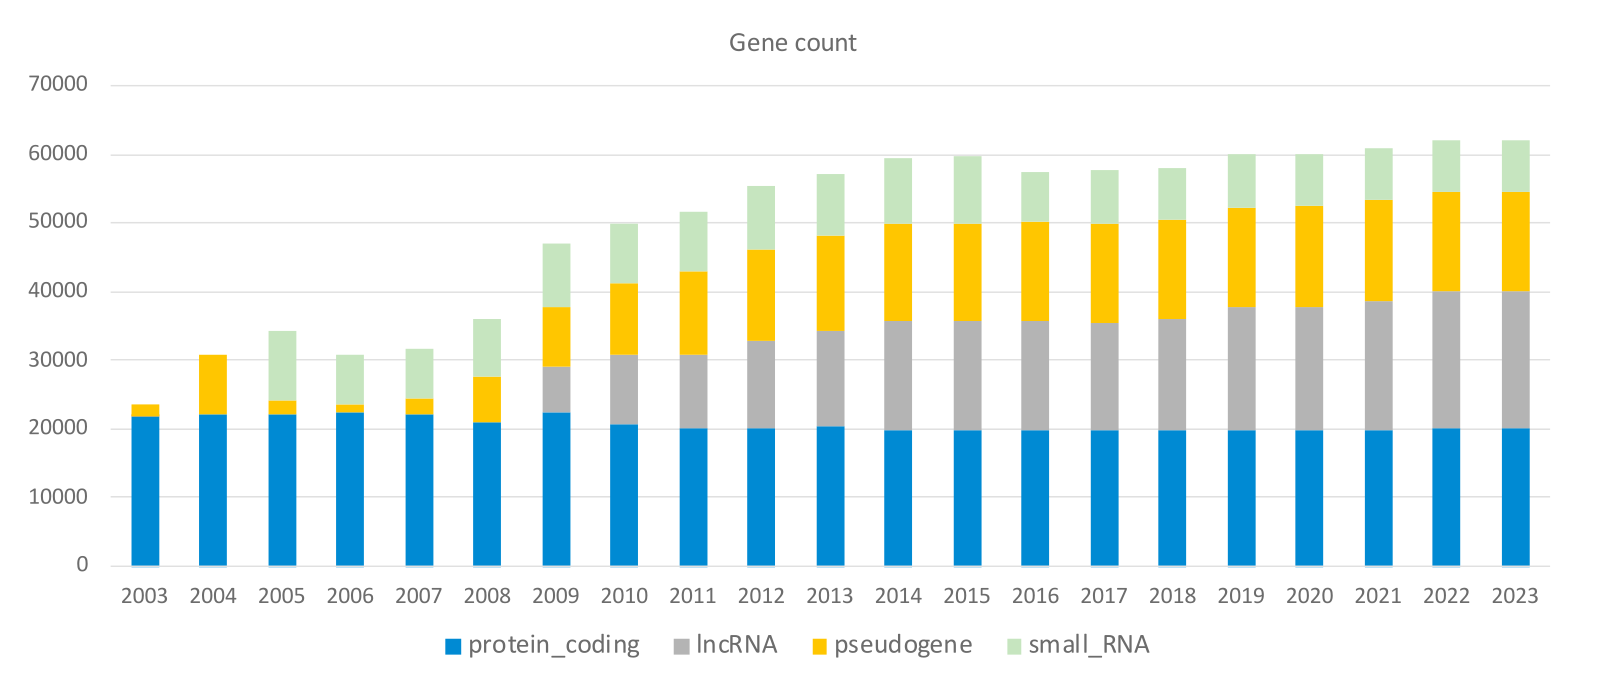
\includegraphics[width=\linewidth]{images/gencode.png}
  \caption{Number of different genes in the gencode annotation during time. Figure taken from paper by \textcite{Guigo2023}}
  \label{fig:gencode}
\end{figure}

\section{Transcriptomic references for scRNAseq}

Having well annotated genome does not solve all the problems related to it.
The complexity of the genome also causes problems for the mapping software.














\iffalse
\section{Key methods and technologies in scRNAseq}

\subsection{Key methods}

All scRNAseq protocols share these main three steps:
isolation of single cells, library preparation and sequencing (\cite{Andrews2018}).

\begin{itemize}
  \item \textbf{Isolation of single cells:} Cells are separated from each other
  and placed into different droplets (microfluidics approach)
  or into different wells (plate-based approach).
  \item \textbf{Library preparation:} The next generation sequencing (NGS) usually requires nanograms or more of DNA,
  and the RNA content in single cells is far from this amount (\cite{Wu2017}).
  Consequently, before sequencing, reverse transcription (RT) and amplification is needed.
  Additionally, usually cell barcode sequences and unique molecular identifiers are attahced to the transcripts (before amplification),
  which later allows one to identify cell of origin for each read and real number of counts.
  \item \textbf{Sequencing:} NGS methods are used for the scRNAseq sequencing.
  Afterwards, acquired data can be processed and analyzed using bioinformatical methods.
\end{itemize}

Even though these steps are common to all scRNAseq protocals,
the variations in details give variations in the results, each one having its own strengths and weaknesses.
In the next section I will overview most popular platforms for scRNAseq.

\subsection{Current scRNAseq Platforms}

As mentioned before, scRNAseq methods mainly can be grouped in two groups: droplet-based and plate-based.

Droplet-based methods (e.g. inDrops (\cite{Klein2015}), Drop-seq (\cite{Macosko2015}),
Chromium by 10X Genomics (\cite{Zheng2017}))
separate cells by placing them into different droplets, which contain hidrogel primers and lysis mix.
Primers usually share a common structure, including barcode sequenes, unique molecular identifiers (UMIs),
PCR handlers and poly-T sequences (\cite{Zhang2019}).
Cell barcodes are sequences used for determining the cell from which a particular read was sequenced
(during sequencing, the content from all droplets is mixed and sequenced at once).
UMIs are used to quantify real amount of RNA in cells
(after amplification, more than one copy of each captured RNA is present).
PCR handlers are used for the amplification, while poly-T sequences are used for capturing RNAs.
An example of primer design can be seen in figure \ref{fig:primer}.
Once cells are in the droplets, cell lysis takes place, RNAs escape the cells and are captured by the primers.
Depending on method,
reverse transcription either takes place directly in the droplets (inDrops, 10X) or after demulsification (Drop-seq).
The next steps usually include RNA fragmentation and PCR amplification, followed by NGS.

Droplet-based methods are high-throughput
(current microfluidic devices are able to generate thousands of above described droplets per second (\cite{Prakadan2017})),
cost-effective, but have low detection rates compared to other methods and
captures only 3' (or 5') ends of transcripts (\cite{Heumos2023}).
Capturing only 3' ends of transcripts might be not a problem when trying to identify cell populations,
however, it masks such processes as splicing variants, thus should be considered carefully when planning experiments.

Plate-based methods (e.g. CEL-Seq2 (\cite{Hashimshony2016}), Smart-seq2 (\cite{Picelli2013}))
separate cells by placing them into different microwells on a plate.
Before this, cells can be sorted using, for example, fluorescent-activated cell sorting (FACS) (\cite{Heumos2023}).
Similarly to droplets, microwells contain lysis buffers and RT mix,
followed by amplification and NGS (\cite{Hashimshony2016}).
Barcodes can be integrated into reverse transcription step similarly as in droplet case.

Overall, plate-based methods have lower throughput, might be more costly and labor-intensive,
but offers recovery of many genes per cell, allows prior sorting and
(for some protocols) it is possible to sequence full transcripts (\cite{Heumos2023}).

In the next sections, we will focus on the droplet-based approaches,
as all the data used in this thesis is generated by droplet-based methods.

\begin{figure}
  \centering
  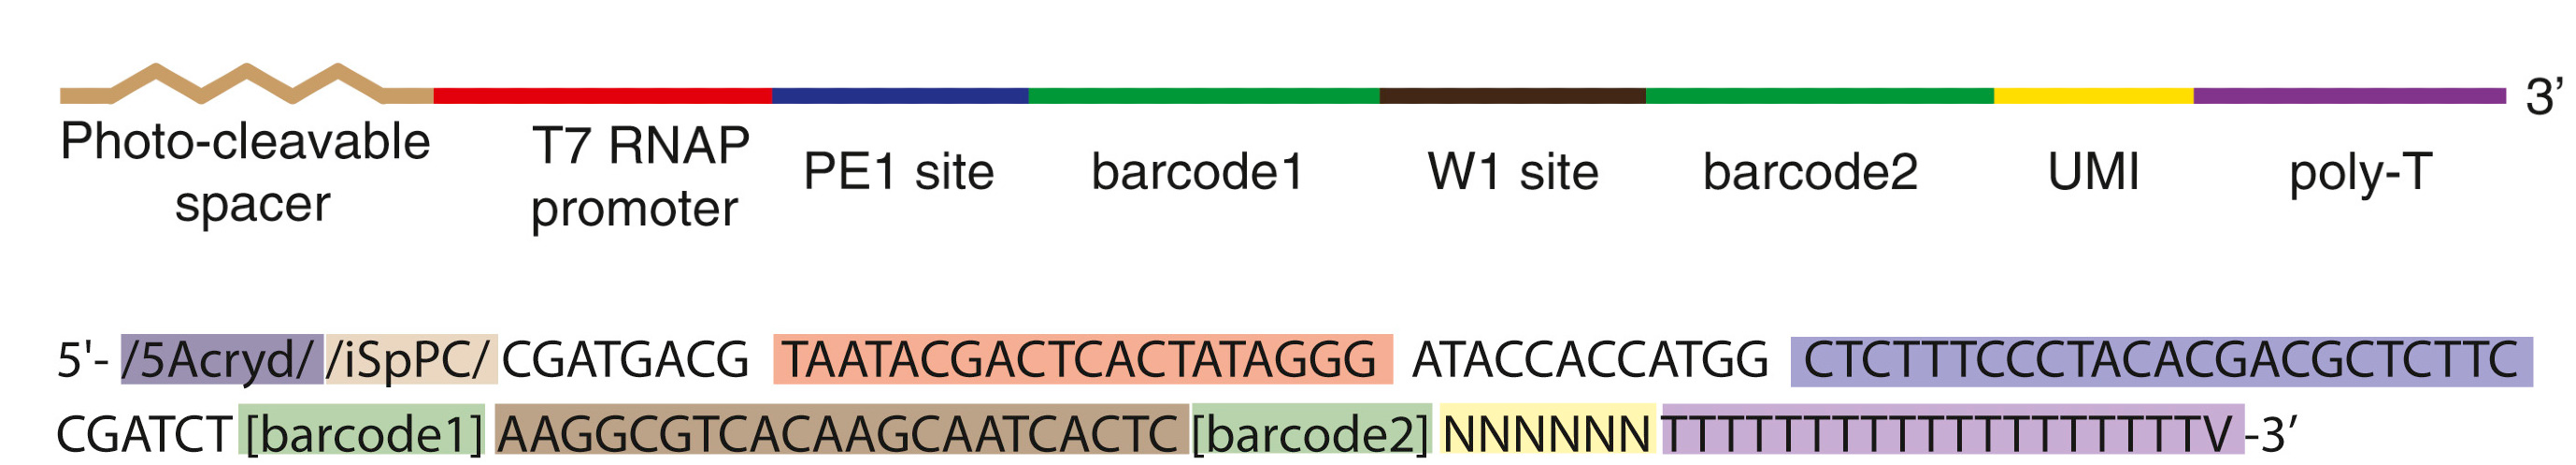
\includegraphics[width=\linewidth]{images/primer.png}
  \caption{Example of barcode (inDrops). The top image contains schematic view, while the bottom one shows example sequence.
           T7RNAP, PE1 and W1 sites here are used for primer assembly,
           while photo-cleavable spacer is used to release primers from the gel beads. Image taken from (\cite{Klein2015}).}
  \label{fig:primer}
\end{figure}

\section{Data quality and challenges in scRNAseq data}

The scRNAseq data offers high resolution insights in the cellular systems, however,
it comes with unique (and non-unique) challenges that need to be overcame to have clean, good-quality data.
In this section I will briefly overview noise sources and data scale challenges.

\subsection{Noise}

The noise in the scRNAseq data can have either biological or technical origin.
The biological noise is always present in the cellular systems due to the stochasticity of all biological processes (\cite{Vaz2017}).
While it is always in the data, more important is to eliminate technical noise.
Technical noise is the artefact of sequencing procedures.
The typical challenge in scRNAseq data is large number of dropout values (and consequently sparse data matrices).
I.e., if there is a zero entry in the cell-gene matrix, is not clear whether the gene was not expressed in the particular cell,
or was expressed but not captured.
This problem is particularly important if one is interested in rare transcripts.

Additionally, droplet-based methods introduce doublets and ambient RNA.
These two will be discussed in sections \ref{sec:preprocessingMatrices} and \ref{sec:imputation}.
In general, when the origin of noise is clear (as in doublets case), it is easier to make computational tools to eliminate it.
For dropout values, it is harder to say whether it is artefact or biological variability, hence eliminating such noise is very complex.

Finally, there are data quality challenges not specific to scRNAseq, such as batch effects.
While those are generally important, we will not focus on them in this review.

\subsection{Data scale and dimentionality}

Another challenge is data scale itself – typical scRNAseq datasets constains thousands of cells and tens of thousands of genes.
Such scales requires very efficiant analysis algorithms (some analysis tools are just too slow for using (\cite{McCalla2023})
and makes interpretability of data harder.
Many analysis pipelines uses dimensionality reduction to reduce the dimensions of the data (more on it in \ref{sec:dimReduction}).

\section{Computational tools and analytical approaches}

\subsection{Raw data processing}

The output of the typical scRNAseq experiment is FASTQ files, containing recorded sequences,
as well as (depending on method) barcode and UMI sequences, and quality scores.
The subsequent processing steps include quality control of FASTQ file (based on quality scores),
filtering dublicate reads (using UMIs), mapping reads to the genome sequence, assigning the reads to the genes,
and finally, counting gene expression per cell (barcode) (\cite{Heumos2023}) (see figure \ref{fig:rawData}).
Usually, all these steps are performed with a single piece of dedicated software,
such as STARsolo (\cite{Kaminow2021}), CellRanger (\cite{Zheng2017}) or others.
It should be noted, that there are variations in the pipeline described above,
depending on many experiment-related (e.g., whether the genome sequence or transcriptone of the study organism is known),
or method-related (e.g., whether UMIs are used in the protocol) factors.
The typical result of such processing is cell-gene matrix (i.e., a matrix where rows represent cells,
columns represent genes, and each entry indicates the number of captured RNAs for a given gene in a specific cell).

\begin{figure}
  \centering
  
\includegraphics[width=\linewidth]{images/rawdata.png}
  \caption{Pipeline of processing raw data.}
  \label{fig:rawData}
\end{figure}

\subsection{Preprocessing of count matrices}
\label{sec:preprocessingMatrices}

Preprocessing of count matrices usually involves these steps:
quality control, normalization and feature selection.

The quality of indidual cells can be evaluated based on several factors, such as mitochondrial gene content
(apoptotic cells tend to have a higher proportion of mitochondrial genes (\cite{Heumos2023})) or
total number of captured genes (very low numbers can be produced by empty droplets).
In some cases, two cells can end up in one droplet,
resulting in count matrix row corresponding to genes from  both cells.
Such matrix entries (doublets) can be filtered by using specialized software
such Scrublet (\cite{Wolock2019}) or scDblFinder (\cite{Germain2022}).
Another source of noise in scRNAseq data is ambient RNA,
which consists of RNA that escapes individual droplets and spreads into the medium or other droplets,
leading to background noise.
Even though the amount of such RNA is not high (in good quality datasets it can be around 2\% (\cite{Young2020})),
removing these RNAs from the count matrix can improve data quality.
This can be achieved by identifying the background noise profile from empty droplets and
adjusting the count matrix accordingly.
There are dedicated softwares,
such as SoupX (\cite{Young2020}), decontX (\cite{Yang2020}), CellBender (\cite{Fleming2023}) and others.

The next step in preprocessing pipeline is normalization.
The goal of normalization is to transform the data so that the variation in gene expression levels is comparable,
making subsequent analysis more efficient (\cite{Ahlmann2023}).
Normalization can also help eliminate biases,
such as differences in sequencing depth when combining data from multiple samples (\cite{Lingen2024}).
There are numerous normalization methods, based on different approaches
(e.g., delta-method-based, residual-based, latent gene expression-based, count-based (\cite{Ahlmann2023})).
Thus, selecting a normalization method should be done carefully, depending on the experimental design.
General recommendations for normalization suggest comparing several methods,
and if the results are similar, opting for the simpler method (\cite{Lingen2024}).
Sophisticated methods do not necessarily show better results, and a recent benchmarking study by \textcite{Ahlmann2023}
has shown that simpler method (particularly the logarithm normalization,
where each element $y$ of count matrix is transformed by formula $y_{trnasformed} = log(y+1)$)
performs as well or better than more advanced methods.

Once the data is normalized and cleaned, one can filter out non-informative genes.
Initially, count matrices contain all the genes that are present in the transcriptome.
However, not all of them are expressed in the sequenced data, or are expressed in negligable numbers (\cite{Heumos2023}).
Therefore, it is common practice to filter such genes (e.g., genes that are expressed in less than three cells).
Moreover, some genes might be expressed in all the cells more or less evenly (housekeeping genes),
which do not provide useful information that could be usefull in, for instance, grouping cells or determining cell types.
Therefore, in many applications, it is beneficial to leave only those genes, that are highly variable between cells.
In such way, the dimensionality of the count matrix is greatly reduced without loosing significant information.
Additionally, genes that are outside the scope of the specific study can also be filtered out.

\subsection{Dimensionality reduction}
\label{sec:dimReduction}

Even after filtering and selecting only highly variable genes, several thousand genes usually remain.
It is not feasible to visualize (and hard to interpret in general) data of such high dimentionality, therefore,
dimensionality reduction is essential step of subsequent analysis.
The idea of dimentionality reduction is simple:
to reduce the dimentions of the data loosing as little information as possible.
There are number dimensionality reduction methods based on different mathematical concepts,
but the most widely used today include
t-SNE (\cite{Hinton2002}), UMAP (\cite{McInnes2018}) and principal component analysis (PCA).
Although the use of these algorithms are supported by some benchmarking studies
(in the study of \textcite{Xiang2021}, t-SNE was showed best performance, while UMAP showed the highest stability),
other benchmarking studies report different findings.
The study of \textcite{Koch2021} suggested that such overlooked methods as
latent Dirichlet alloacation (LDA) and PHATE show best performance.
Meanwhile \textcite{Sun2019} provided guidelines for choosing dimensionality reduction method
depending on downstream analysis tasks, and in their results UMAP and tSNE were not on the top choices.
Thus, while UMAP and t-SNE remain the most popular methods in the field,
it is worth considering alternative methods as well.

\subsection{Clustering and other analyses}

One of the most common tasks of scRNAseq data analysis is to identify and classify cell populations (\cite{Andrews2018}).
This task requires to assign cells to different groups (clusters),
such that cells in the same clusters are similar and distinct from cells in other clusters.
There is a great variety of clustering algorithms available,
including k-means, hierarchical and consensus clustering (\cite{Peng2020}).
Benchmarking studies suggest that "no individual scRNA-seq clustering algorithm can capture true clusters and achieve
optimal performance in all situations" (\cite{Peng2020}).

Clustering is usually followed by cell typing (i.e., assigning cell type to the identified clusters),
which is done by finding cell type specific markers
or using automatic (machine learning) tools such as CellTypist (\cite{Dom2022}).
The subsequent steps in the analysis depend on the focus of the particular study and can include
analysis of the dynamics of cellular systems (RNA velocity, pseudotime),
inferring gene regulatory networks (GRNs), and more.

\section{Enhancing scRNAseq data}

Given the challenges associated with scRNAseq data, there have been attempts to improve the quality of such data.
In this section, I will provide an overview of two methods: data imputation and enhancing the transcriptomic reference.

\subsection{Data imputation}
\label{sec:imputation}

One of the challenges present in scRNAseq data is the large number of dropout values.
Dropout values refer to instances where gene expression is present in a cell but is missed in the scRNAseq data.
This problem can mask important relationships between genes and complicate downstream analysis (\cite{Wang2022}).
To impute dropout values, many tools have been suggested.
These methods can be divided into four categories:
model-based methods (bayNorm (\cite{Tang2019}), BISCUIT (\cite{Azizi2017}), SAVER (\cite{Huang2018}) etc.),
low-ranked matrix-based (ALRA (\cite{Linderman2022}), ENHANCE (\cite{Wagner2019}), scRMD (\cite{Chen2020}) etc.),
data smoothing methods (e.g. KNN-smoothing (\cite{Wagner2017}), MAGIC (\cite{Dijk2018}) etc.) and
deep learning methods (e.g. DCA (\cite{Eraslan2019}), DeepImpute (\cite{Arisdakessian2019}) etc.) (\cite{Wang2022}).

The study by \textcite{Dai2022} has shown that imputation methods are advantageous for recovering gene expression,
and among these methods, deep learning-based ones,
such as DCA, DeepImpute, scIGANs (\cite{Xu2020}) show the best performance.
However, it was also shown that imputation methods can introduce false positives.
In the study by \textcite{Andrews2019}, it was shown that data smoothing methods (e.g. MAGIC, KNN-smoothing)
generate most false positives among the different types of methods,
but other methods can generate relatively large number of false positives as well, depending on the dataset.
Data imputation does not necessarily improve downstream analysis
(e.g, it was shown that imputation doesn't improve inference of gene regulatory networks (\cite{McCalla2023})),
therefore one should carefully choose whether to impute data and which method to use.

\subsection{Enhancing transcriptomic reference}

One of the problems that scRNAseq is facing is the complexity of the genome.
The "raw" human transcriptomic reference (a file containing information about genes)
contains over 60000 genes (\cite{Frankish2022}).
Not all of these genes are expected to be captured by scRNAseq data
Thus, a simple approach to improving the transcriptomic reference is to filter out the genes
that are not expected to appear in scRNAseq data.
In this way, events where two genes overlap in the genome, but one is not expected to appear in the scRNAseq data,
are resolved, allowing alignment tools to more easily assign reads from these regions to the correct genes.
This approach is used in publicly available 10X transcriptomic references (\cite{Zheng2017}).
Even though it improves mapping performance, it does not address all the issues with the transcriptomc reference.

\textcite{Pool2023} has suggested three steps to enhance transcriptomic reference:
including reads mapped to intronic sequence to the analysis, extending 3' ends of some genes and
resolving overlaps between certain genes.
The first suggestion is not new in the field of scRNAseq.
There are concepts such as RNA velocity based on spliced an unspiced RNA ratio (\cite{Manno2018}),
showing that such including intronic reads in the analysis can provide valuable information.
Moreover, most mapping tools (e.g. STARsolo, CellRanger) contains options
to use either only exonic parts or full genes for read alignment.
The second suggestion is based on the observation,
that scRNAseq data often contains peaks of reads just after the 3' end of genes. 
While the exact biological reasons for this are unclear,
it makes sense to associate these reads with the genes they are closest to. 
The third suggestion focuses on resolving overlaps between genes.
Reads from such overlapping regions are often unassigned to any gene,
but in some cases, it is more likely that they originate from one gene rather than another.
Overlapping gene resolution aims to address this by deleting or shortening some genes in the transcriptomic reference.

Although \textcite{Pool2023} proposed the tool for such tasks, the tool is not without limitations:
some aspects of it are debatable (such as thresholds used), some seem unnecessarily
(e.g. handling exon and intron sequences when most alligning tools provide option for this),
and the process still requires a significant amount of manual work.
Thus, there remains a need for a more comprehensive tool for enhancing transcriptomic references,
which will be addressed in this thesis.

Another aspect, that should be taken into account, is that not all genes are known and annotated, even for such well-studied species as human.
Several tools were developed to predict de novo genes, such as AUGUSTUS (\cite{Stanke2008}), geneid (\cite{Blanco2007}), Gescan (\cite{Burge1997}),
SPG2 and SIB predictions (\cite{Prediction}).
Nevertheless, none of them are perfect, and new genes that were not predicted by those tools are defined,
as can be seen from conctantly updated human transcriptomes.
Hence, the need for identifying new gene candidates remains, especially using other methods.

\section{Getting insights from scRNAseq data}

\subsection{Trajectory inference}

The scRNAseq data is static snapshot due to a destructive nature of sequencing methods,
which give raise to the challenges that could be only overcome with modelling approaches.
Trajectory inference methods aim to reconstruct the dynamics of cellular processes of interest,
such as development, differentiation or immune response (\cite{Deconinck2021}).
These inference methods assign a numerical value referred as pseudotime for each cell, and based on it,
cells can be organized along the pseudotemporal axis and may recapitulate biological dynamical processes (\cite{Wang2021}).
Inference of pseudotime usually firstly reduces dimentionality of the data, and then applies either clustering or graph approaches
for placing cells into the trajectory structures (\cite{Deconinck2021}).
The scRNAseq data contains both spliced and unspliced RNA transcrips, which provide additional temporal information.
Based on it, there were proposed RNA velocity models, that aim to find the vectors predicting future state of individual cells (\cite{Manno2018}).

There are plenty of methods both for pseudotime ordering and RNA velocity, and before using them,
one should take into account the assumptions and limitations of individual models.
Such assumtions often include the type of trajectories (e.g. branching, linear etc.), systems state (e.g. steady state, dynamical) and others.

\subsection{Inferring gene regulatory networks}

Understannding regulatory relationships between genes is one of the main problems in system biology and medicine (\cite{Lamoline2024}).
High resolution scRNAseq data offers a chance to do this via inference of gene regulatory networks (GRNs).
GRN is a graph representing relationships between transcription factors and genes they control,
i.e. it is a graph where genes are represented by nodes and their relationships (activating or inhibiting) are represented by edges.
Various mathematical concepts are used in GRN inference algorithms, including
correlation, mutual information, regression, Baysean networks, boolean networks, differential equations and others (\cite{Akers2021}).

Even though there are plenty of inference models, there are no single methods that would be best in all situations.
Moreover, performance of such algorithms often shows poor results, on global metrics similar to randomly creating GRNs.
This was shown in the benchmarking study by \textcite{McCalla2023}.
In the study 13 inference algorithms were compared, and none of them were best on different datasets and gold standards used.
However, while not showing great performances on global metrics, methods were able to extract some useful local information
(e.g. on some specific transcription factors that are major regulators in some cell lineages).

All in all, while there are plenty of inference algorithms, none of them are perfect,
but can be used to extract some information about cellular systems.

\subsection{Integrative approaches}

The scRNAseq data alone does not capture all the relevant information of cellular system,
therefore good inprovement of analysis is to incorporate other modalities of single cell data (\cite{Heumos2023}).
For example, CITE-seq allows to simultaneously measure gene expression and surface protein abundance (\cite{Mercatelli2021}).
Also, it is possible to capture both transcriptomic and epigenomic features of single cells
(e.g. scM\&T-seq (\cite{Angermueller2016}) allows measure transcriptome together with DNA methylation).
While such approaches supplies additional information about the cellular systems,
they also give rise to additional chalenges when trying to integrate such data.
Such challenges comes from high degrees of missing data, noise, and the scale of datasets,
which can potentially span millions of cells (\cite{Argelaguet2020}).
There are plenty of tools designed for such data integration, including MOFA+, totalVI, WNN and multiVI (\cite{Heumos2023}).

\section{Current limitations and future perspectives}

While scRNAseq data has attracted significant interest within the scientific community,
and numerous tools and methods have been developed for its analysis, substantial challenges remain.
\textcite{Lahnemann2020} identified four major challenges in the field of scRNAseq data science:
addressing data sparsity, defining flexible statistical frameworks for identifying complex differential patterns in gene expression,
mapping single cells to reference atlases, and advancing trajectory inference.

The issue of data sparsity, briefly discussed in section \ref{sec:imputation}, arises when algorithms rely solely on internal data,
which can amplify signals artificially.
This highlights the need for tools that integrate external information, such as reference atlases.
Regarding differential analysis, although scRNAseq datasets capture more detailed information than bulk datasets,
methods specifically tailored for single-cell data often do not outperform bulk methods (\cite{Soneson2017}),
indicating room for significant improvement.

The construction of atlases and reference mapping can reduce considerable manual work, and with the continuous growth in available data,
the demand for such tools is increasing (\cite{Heumos2023}).
While some automatic annotation tools are available (\cite{Dom2022}), most focus on healthy samples,
underscoring the need for reference atlases covering a wider range of states, diseases, and organisms (\cite{Heumos2023}).

Most current trajectory inference methods are limited to scRNAseq data alone.
Incorporating additional data modalities, such as epigenetics or proteomics,
would enhance our understanding of dynamic cellular processes at a systems level (\cite{Lahnemann2020}).

Two other critical topics in scRNAseq data science are the development of end-to-end pipelines and regular benchmarking (\cite{Heumos2023}).
The former is essential due to the rapid expansion of scRNAseq data, while the latter would facilitate
the selection of appropriate tools—especially as there are now over 1,700 tools for scRNAseq data analysis (\cite{scrnatools}).

Finally (and most importantly in the context of this project), there is a need for enhanced transcriptomic reference,
which would allow to include more data in the downstream analysis.
This enhancement could be either based on adjusting the existing references, or by including new genes,
that need to be predicted and confirmed.
\fi


\chapter{METHODS}
\section{Data}

In this thesis following publically available datasets from scRNAseq experiments were used.

\subsection{PBMC}

This dataset is publically available in 10X Genomics website.
In this experiment, human peripheral blood mononuclear cells (PBMCs) were extracted from fresh whole peripheral blood samples obtained from StemExpress. PBMCs were isolated using SepMate density centrifugation methods.
The library was generated from around 8000 cells (5140 cells recovered) using the Chromium Single Cell 3' v3.1 Reagent Kit,
and sequenced on Illumina NovaSeq 6000 to a read depth of approximately 35000 mean reads per cell.
The transcript reads have length of 90bp.
All this information (and more) is available at
\href{https://www.10xgenomics.com/datasets/5k-human-pbmcs-3-v3-1-chromium-controller-3-1-standard}{10X Genomics website}.

\section{Enhancing transcriptomic reference}

The code for enhancing reference was written in R, additionally using some command line tools (the full script is available in appendices).
The code was run on the linux environment in high performance cluster.
Here is provided general description of the code pipeline.

\begin{enumerate}
  \item \textbf{Generating gene location bed file}
  
  In this step, bed file is generated from the initial gtf file.
  The gtf file contains detailed description of every gene, including all exons of genes, hence it contains several lines per gene.
  The resulting bed file is much simpler, having only one line per gene, containing information about its location (chromosome, coordinates, strand).

  \item \textbf{Isolating intergenic reads}
  
  In this step, intergenic reads are isolated from the bam file.
  Extraction is based on three criterions:
  the reads must be unassigned to any gene (i.e. have "GN:Z:-" tag),
  reads must not intersect with any gene location (for this task we use previously generated bed file),
  and reads must have intact cell barcodes and UMIs (checked by their length).
  
  \item \textbf{Creating gene extension candidate list}
  
  It this step, it is checked which genes could be potentially be extended to include reads close to their 3' ends.
  The list is generated which contains numbers of reads present within the threshold distance near the 3' end of each gene.
  This list will later be used for choosing which genes to extend.
  
  \item \textbf{Clustering intergenic reads}
  
  In this step, intergenic reads are clustered, as single reads are more likely artifacts, while clusters of reads may be biologically relevant.
  
  \item \textbf{Identifying overlapping genes}
  
  The overlapping genes (genes that have overlaps with at least one other gene) are identified.
  
  \item \textbf{Resolving overlaps}
  
  In this step, the list that specifies which genes to delete or shorten, is created.
  The overlapping genes resolution startegy is as follows:
  
  \begin{enumerate}
    \item If the distance between 3' ends is larger than threshold set, shorten downstream gene.
    \item If the distance is shorter, shorten or delete the one that has lower priority score.
    \item Otherwise leave for the manual inspection.
  \end{enumerate}
  
  The priority scores are debatable, here I have preferred protein-coding genes versus other types.
  After this step, manual curation of the lists can be done.
  
  \item \textbf{Final reference assembly}
  
  The final transcriptomic reference is assembled.
  It takes into account gene 3' end extension, gene overlaps and includes intergenic reagions that have large clusters of reads.

\end{enumerate}


\chapter{RESULTS}
\section{Intergenic regions}

14 datasets were analysed from various tissues (blood, brain, eye, lung).

Give here statistics about how many there are unassigned reads per sample, i.e. why it is significant.

Also here goes the clustering using only intergenic regions.

for each  intergenic regions were found that contained sufficient amount of unassigned reads,
as described in method section (threashold was set at 5 CPM).
'Intergenic' is used here in a strand specific manner, i.e. the 'intergenic' region can be located on opposite strand of known gene.
The lists of regions from all samples were combined and filtered by the number of samples in which they were detected,
resulting in a list of 2590 intergenic regions.
Of them 147 were not on the opposite strand of known genes, and will be refered from now on as 'isolated'.
Those that are on the other strand of known genes, will be refered as 'antisense'.

\subsection{Isolated intergenic regions}

The intergenic regions that are far from known genes and contain reads might indicate novel genes.
To check whether they are not artifacts, several aspects were considered:
\begin{enumerate}
  \item Whether they are differentially expressed on any samples, i.e. are they specific to some cell types.
  If yes, then it strongly suggests, that they have biological origin and are not artifacts.
  \item Whether there are AT-rich sequences (10 consecutive A/Ts) nearby (checked up to 500 bp upstream).
  This could explain polymerase binding (however, not explain if this is a valid gene, or just an error).
  \item Whether there are open chromatin regions upstream (which is often the case if the gene is actively transcribed).
  \item Conservation score – coding regions tend to be more evolutionary conserved than non-coding regions.
\end{enumerate}

\paragraph{Differential expression analysis}

To check whether an intergenic region is differentially expressed, firstly all datasamples were clustered.
For \textit{PBMC\_10x} samples, it was done using CellTypist (which as well annotates cells),
and for other samples, it was done with 'leiden' algorithm, parameters were chosen manually,
such that overall number of clusters would be similar between similar datasets (i.e. in all \textit{lung} samples there were 5 clusters achieved),
and would visually approximatelly coincide with structures that can be seen in the umaps.
All UMAPs colored by the clusters can be seen in the appendix \ref{fig:clusterings}.

After filtering those regions that were differentially expressed (tresholds were used 0.01 for adjusted p-value and 0.5 for 'logfoldchange'),
the 29 differentially expressed isolated intergenic regions were found.
Some examples can be seen in Figure \ref{fig:isolatedDGE}.

\begin{figure}[htbp]
\centering
\begin{tabular}{cc}
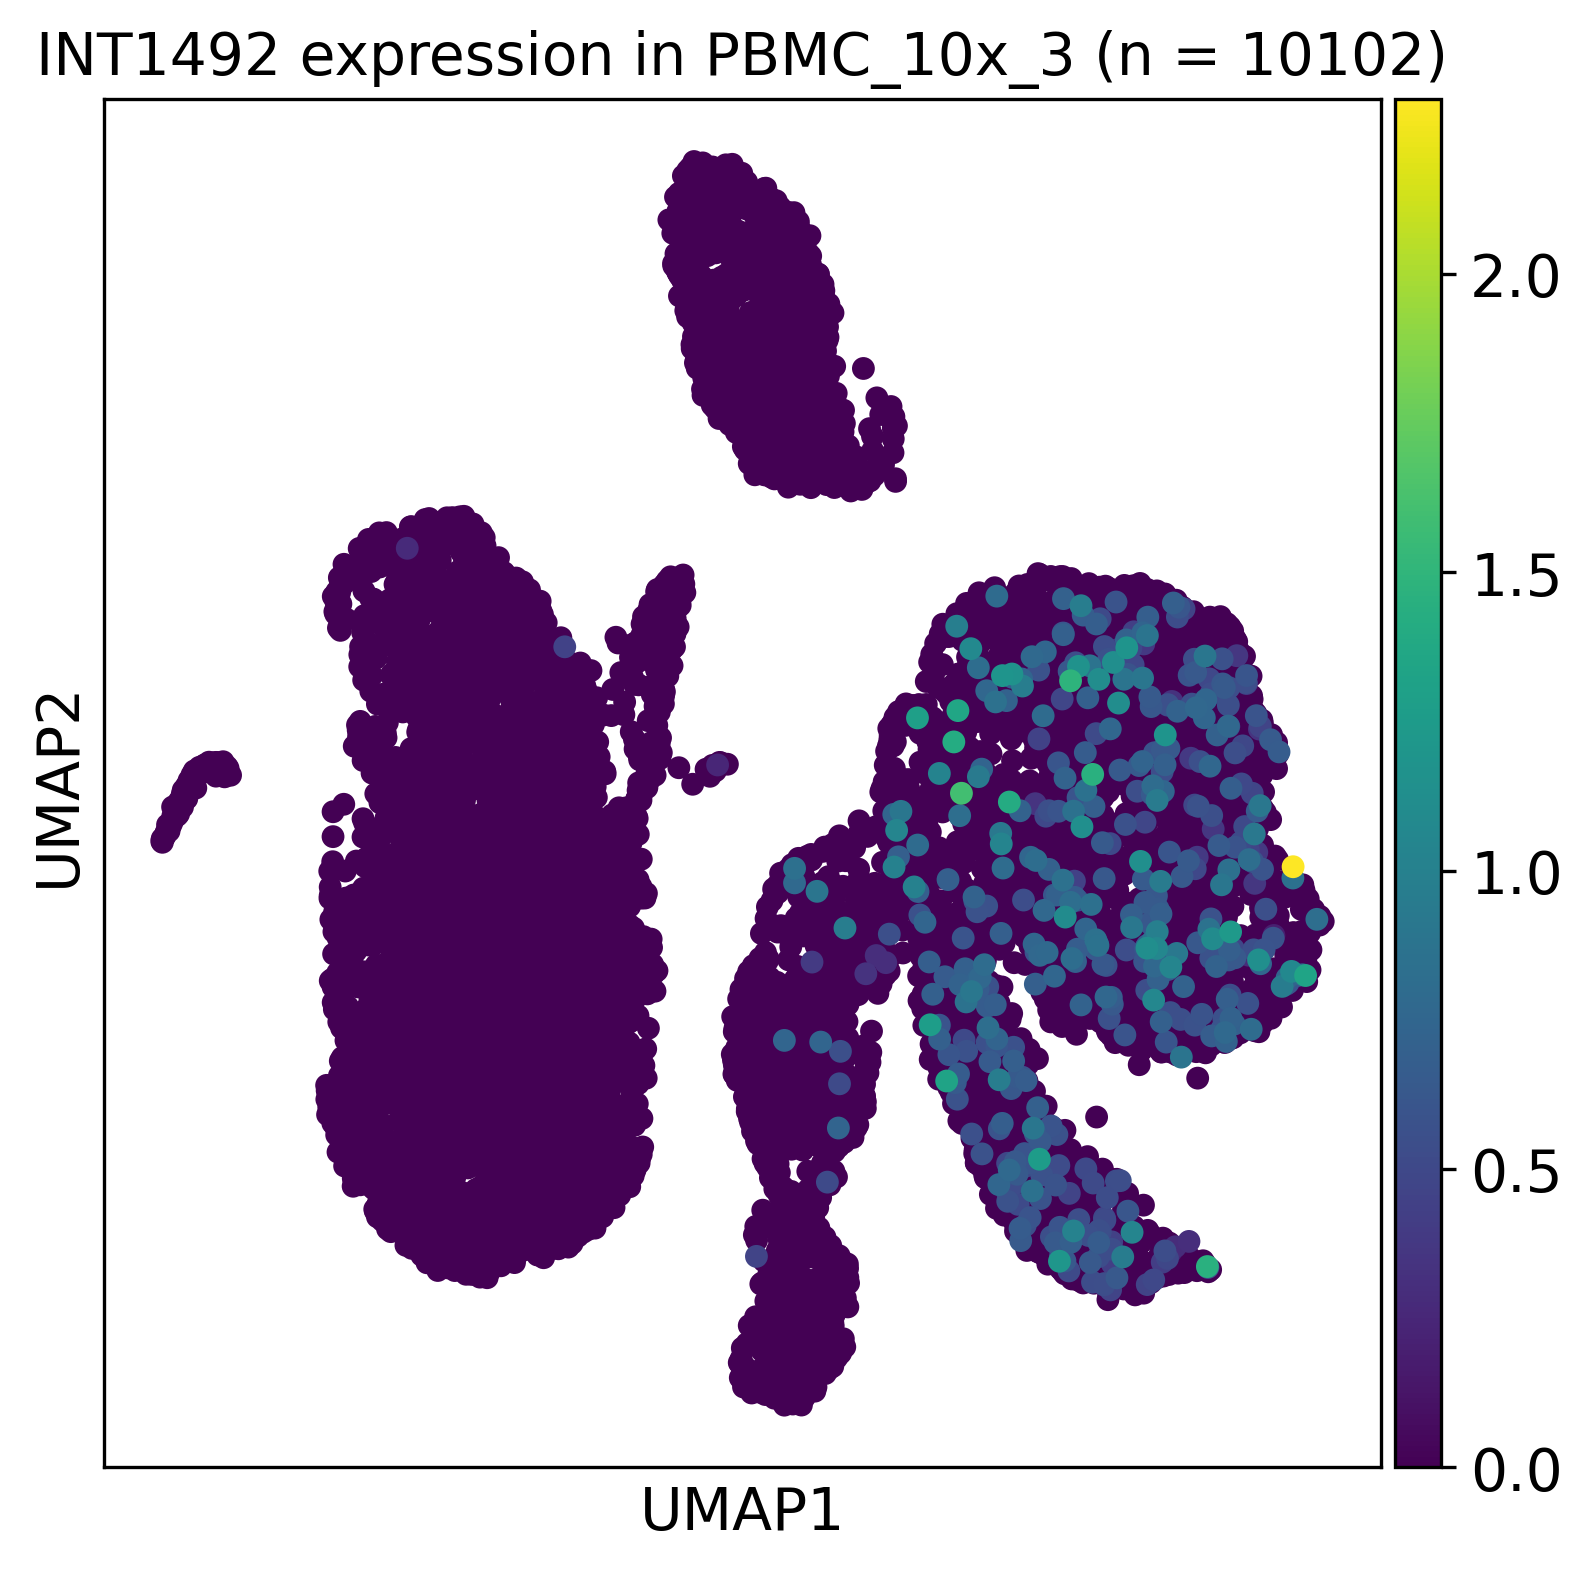
\includegraphics[width=0.45\textwidth]{images/isolatedDGEexamples/INT1492_PBMC_10x_3.png} &
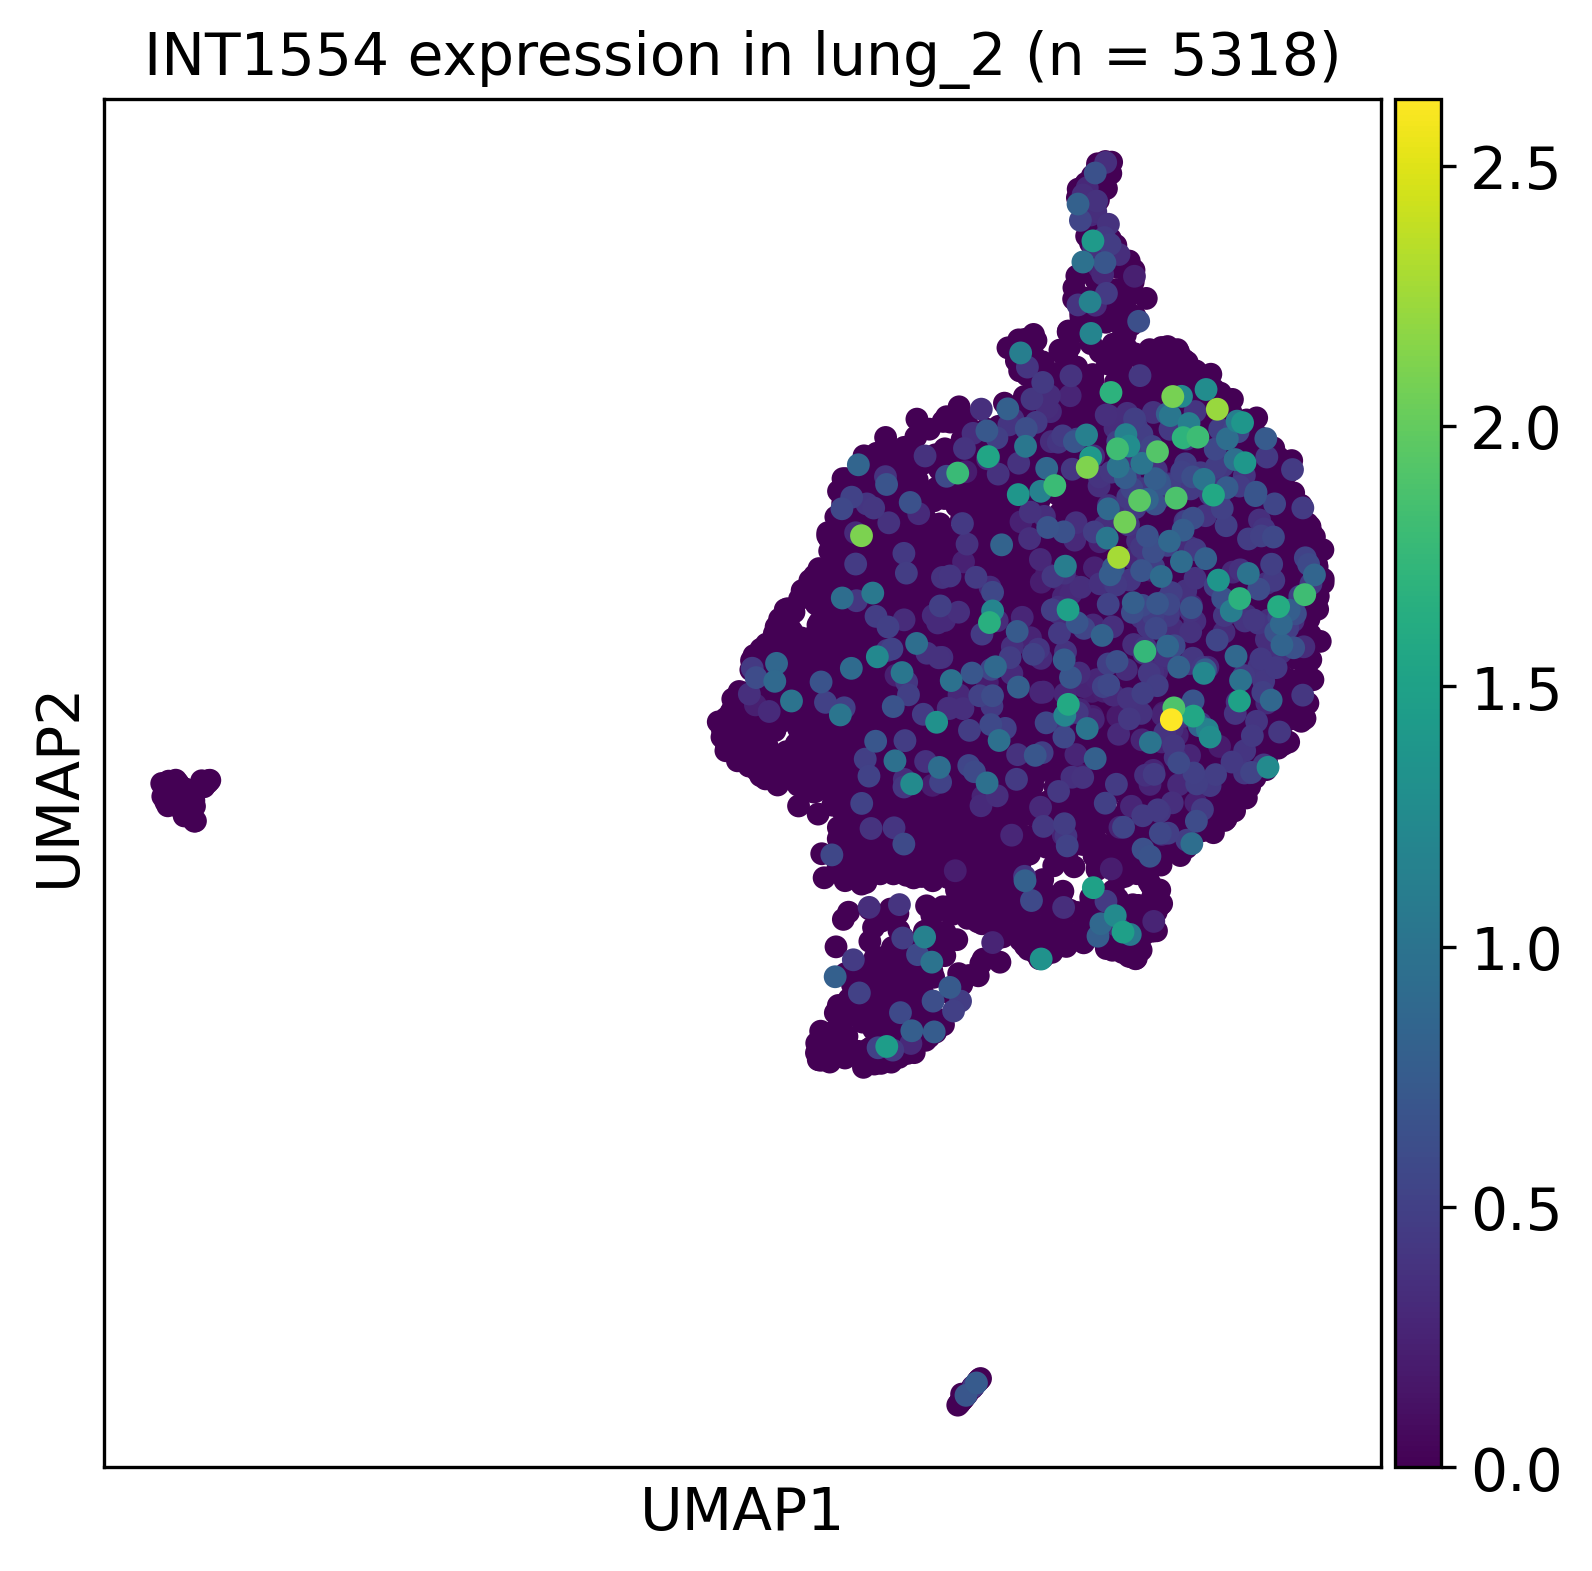
\includegraphics[width=0.45\textwidth]{images/isolatedDGEexamples/INT1554_lung_2.png} \\
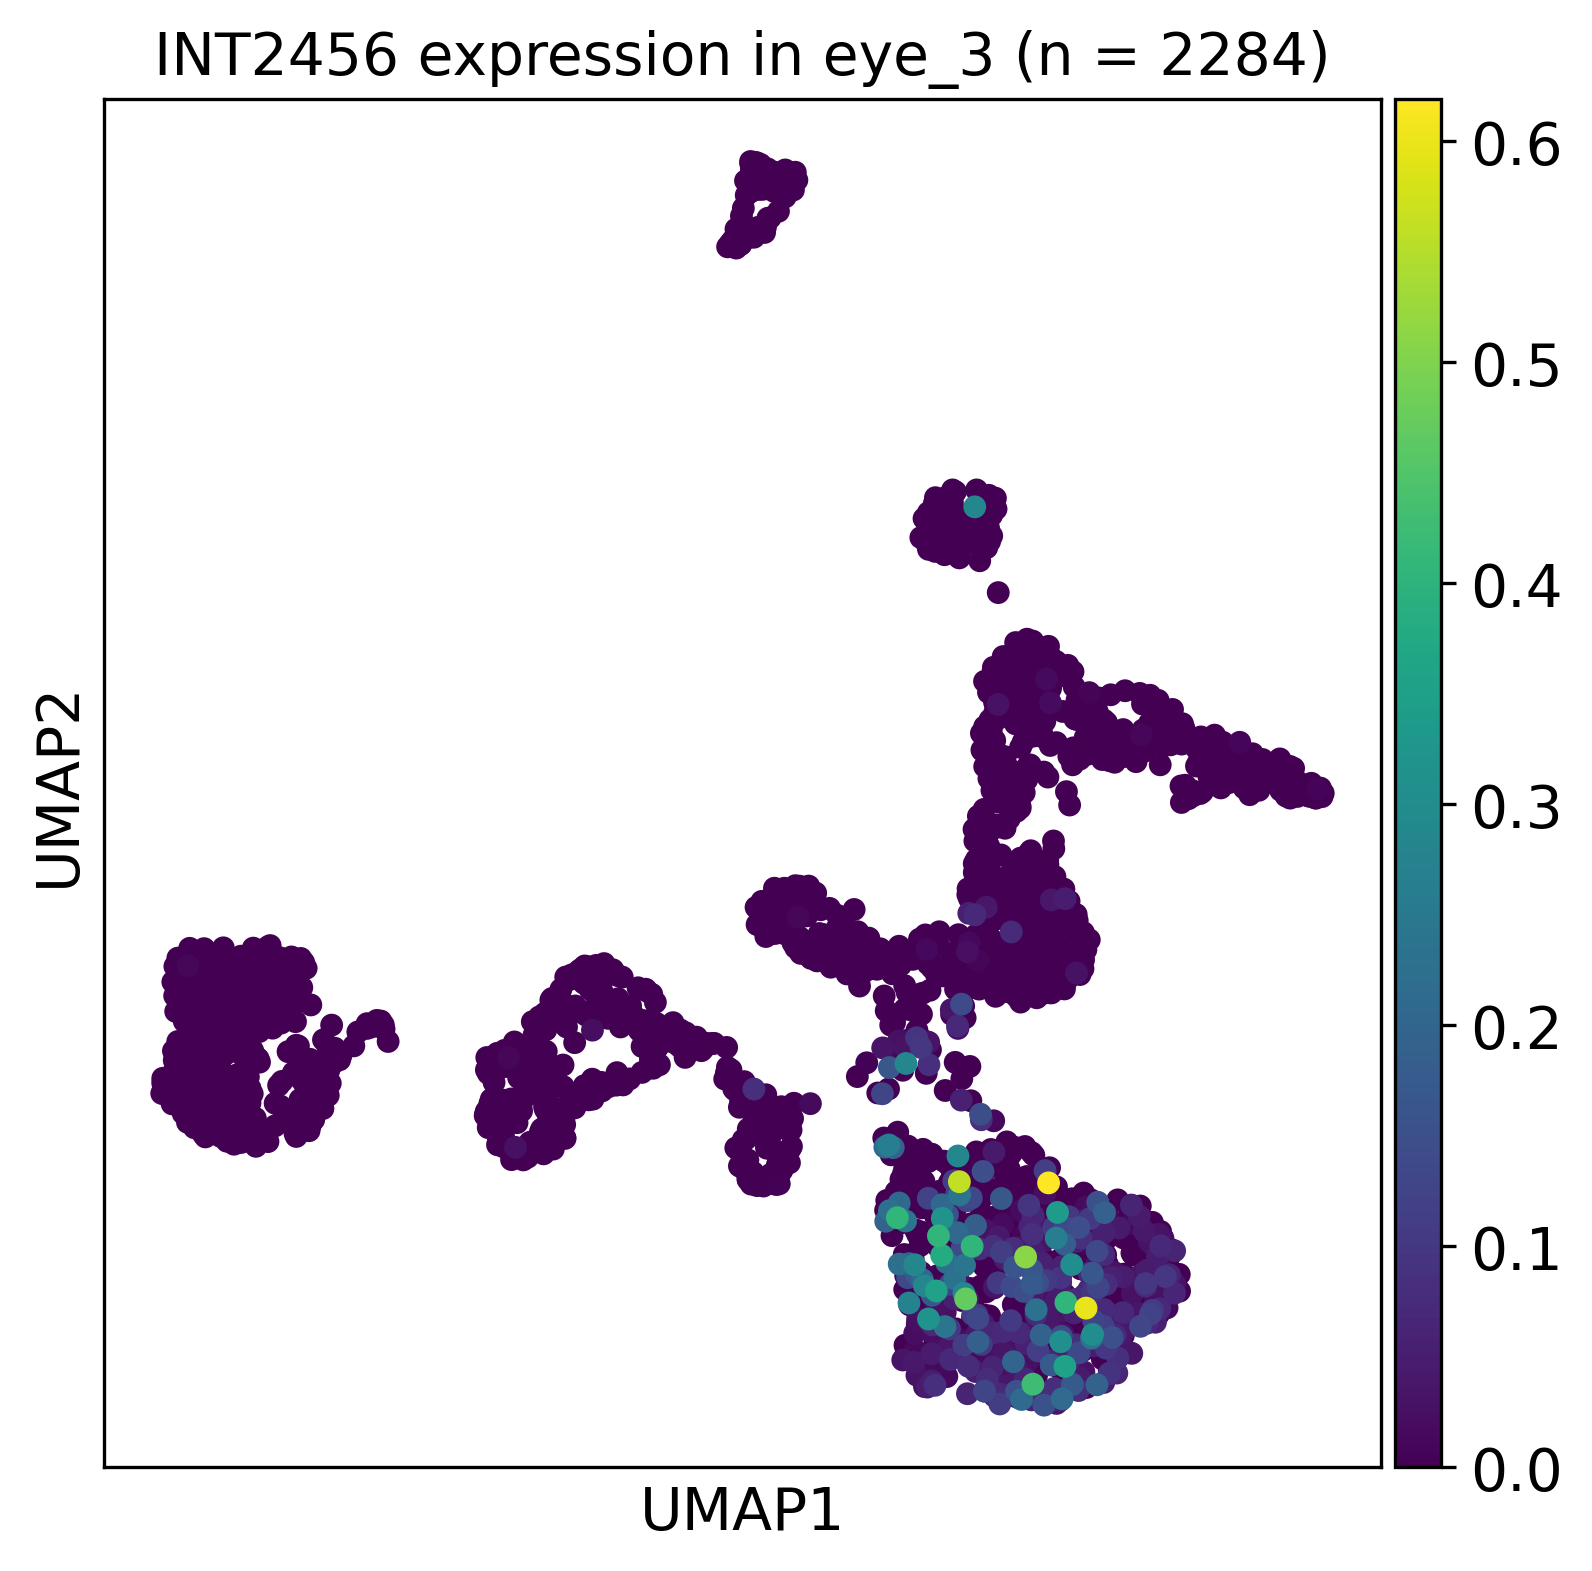
\includegraphics[width=0.45\textwidth]{images/isolatedDGEexamples/INT2456_eye_3.png} &
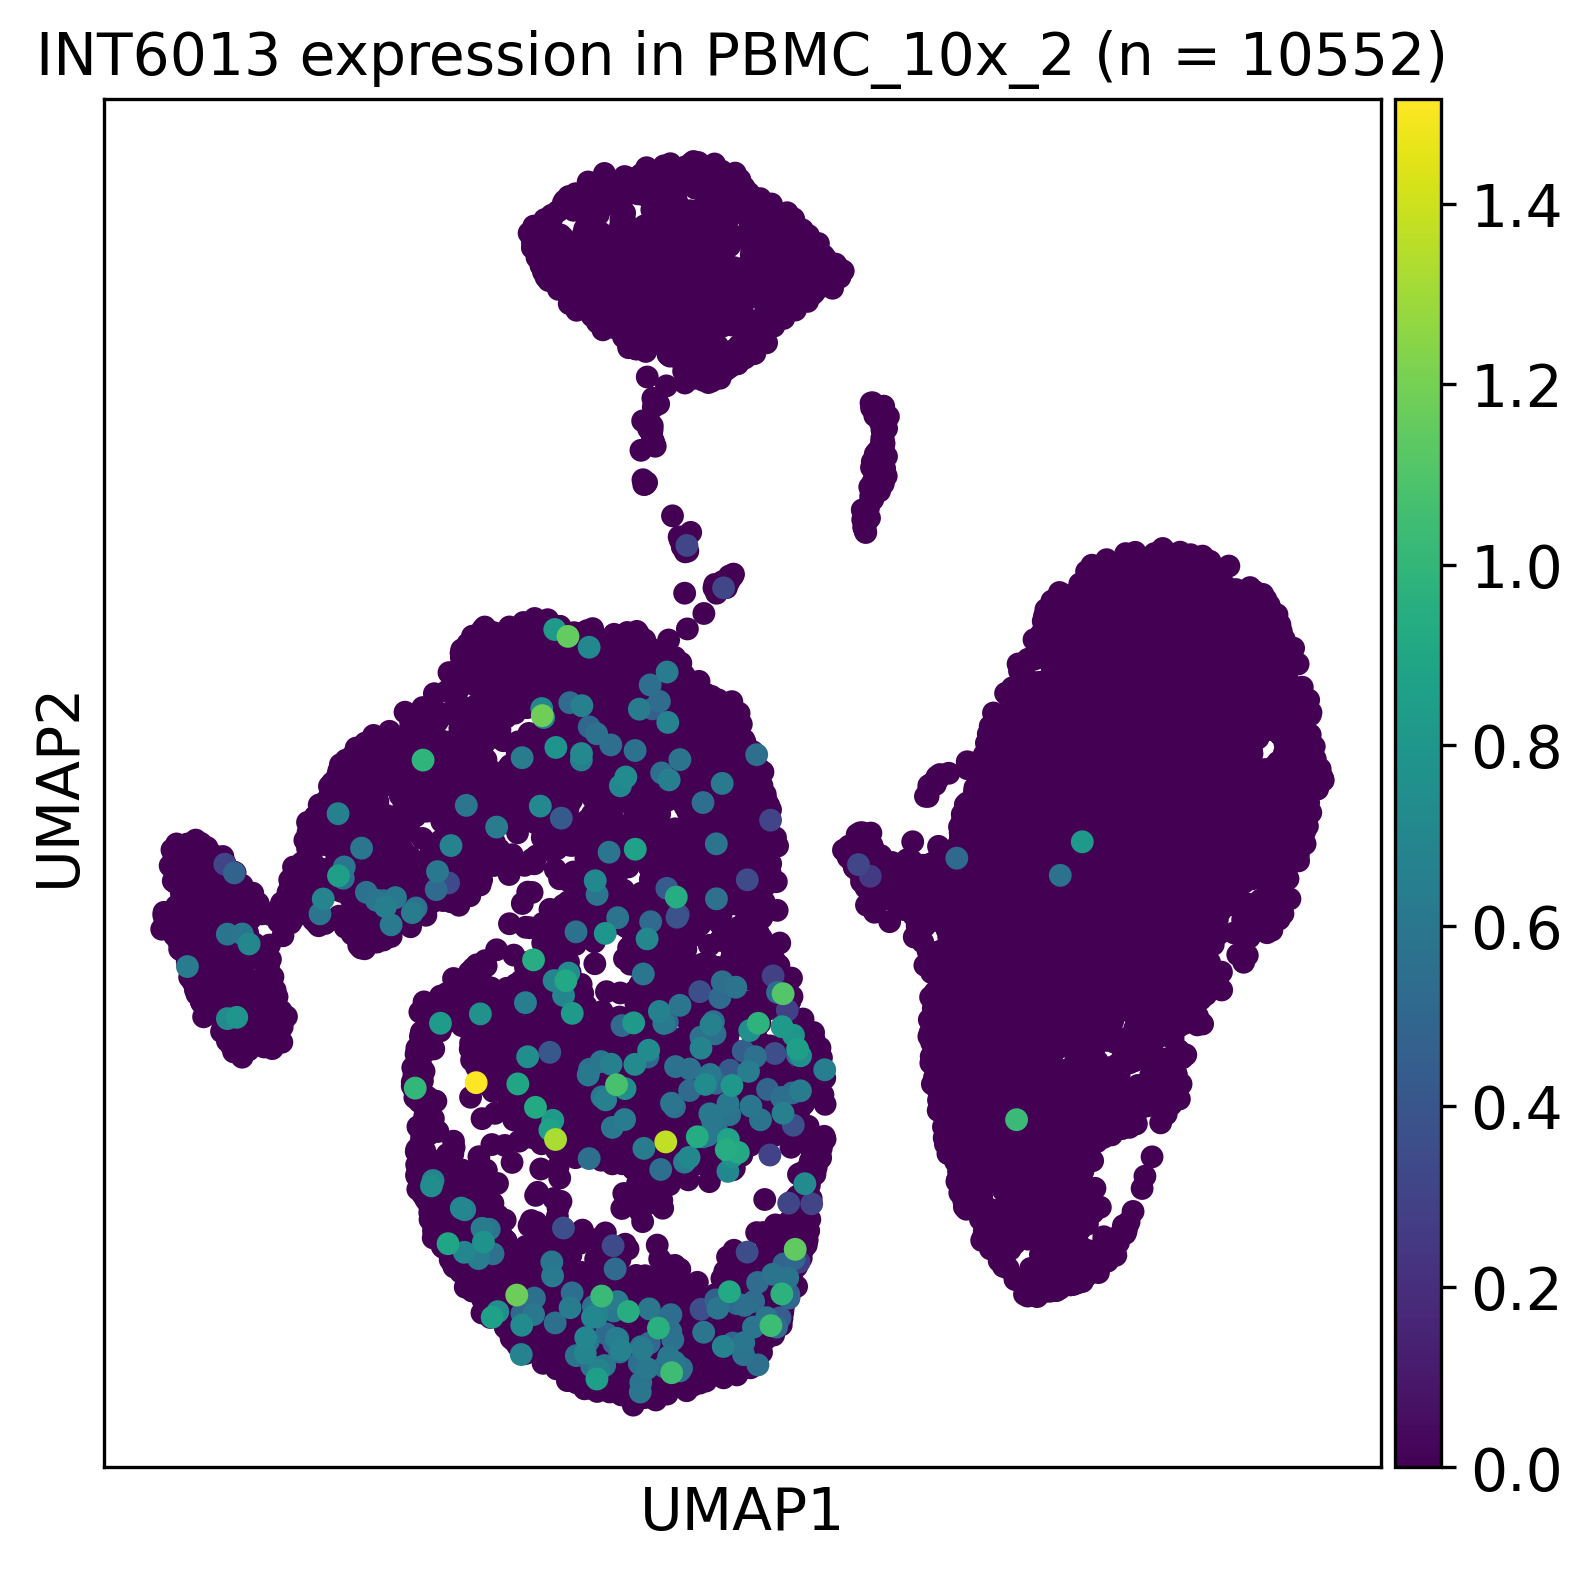
\includegraphics[width=0.45\textwidth]{images/isolatedDGEexamples/INT6013_PBMC_10x_2.png} \\
\end{tabular}
\caption{Examples of differentially expressed isolated intergenic regions.}
\label{fig:isolatedDGE}
\end{figure}

\paragraph{AT-rich regions}

AT-rich regions (here defined as 10 consecutive A's or T's, allowing one 'error', i.e. other nuucleotide)
were looked upstream from the 3' ends of the isolated intergenic regions, and the first hits were reported.

The distances from isolated intergenic regions to such AT-rich regions varied,
with mean 938.537 and median 508, the histogram can be seen in the Figure \ref{fig:distancesATrich}.
To check how these numbers support the claim that those locations are not noise,
distances to AT-rich regions were found from 10000 random locations in the genome and from 10000 3' ends of randomly selected genes.
The results can be seen in the Table \ref{tab:distancesATrich}.
As can be noticed, distances are larger for both the randomly selected genes and randomly selected genes.
Interestingly, distances from random locations to AT-rich regions are on average smaller than from the 3' end of randomly selected genes.
This could be explained by the fact that we are looking for these AT-rich regions upstream from the 3' ends,
meaning that all gene bodies (which typically should not contain AT-rich sequences) are added to those distances.
Also, one could conclude, that if there are genes in between those isolated intergenic regions,
they are potentially small (assuming that AT rich sequences should be found near the 5' ends).

\begin{table}[htbp]
  \centering
  \begin{tabular}{l|cc}
    \toprule
     & mean & median  \\
    \midrule
    intergenic & 938.537 & 508 \\
    random 3' ends & 1391.019 & 849 \\
    random locations & 1123.194 & 682 \\
    \bottomrule
  \end{tabular}
  \caption{The distances to the closest AT-rich regions.}
  \label{tab:distancesATrich}
\end{table}

\begin{figure}
  \centering
  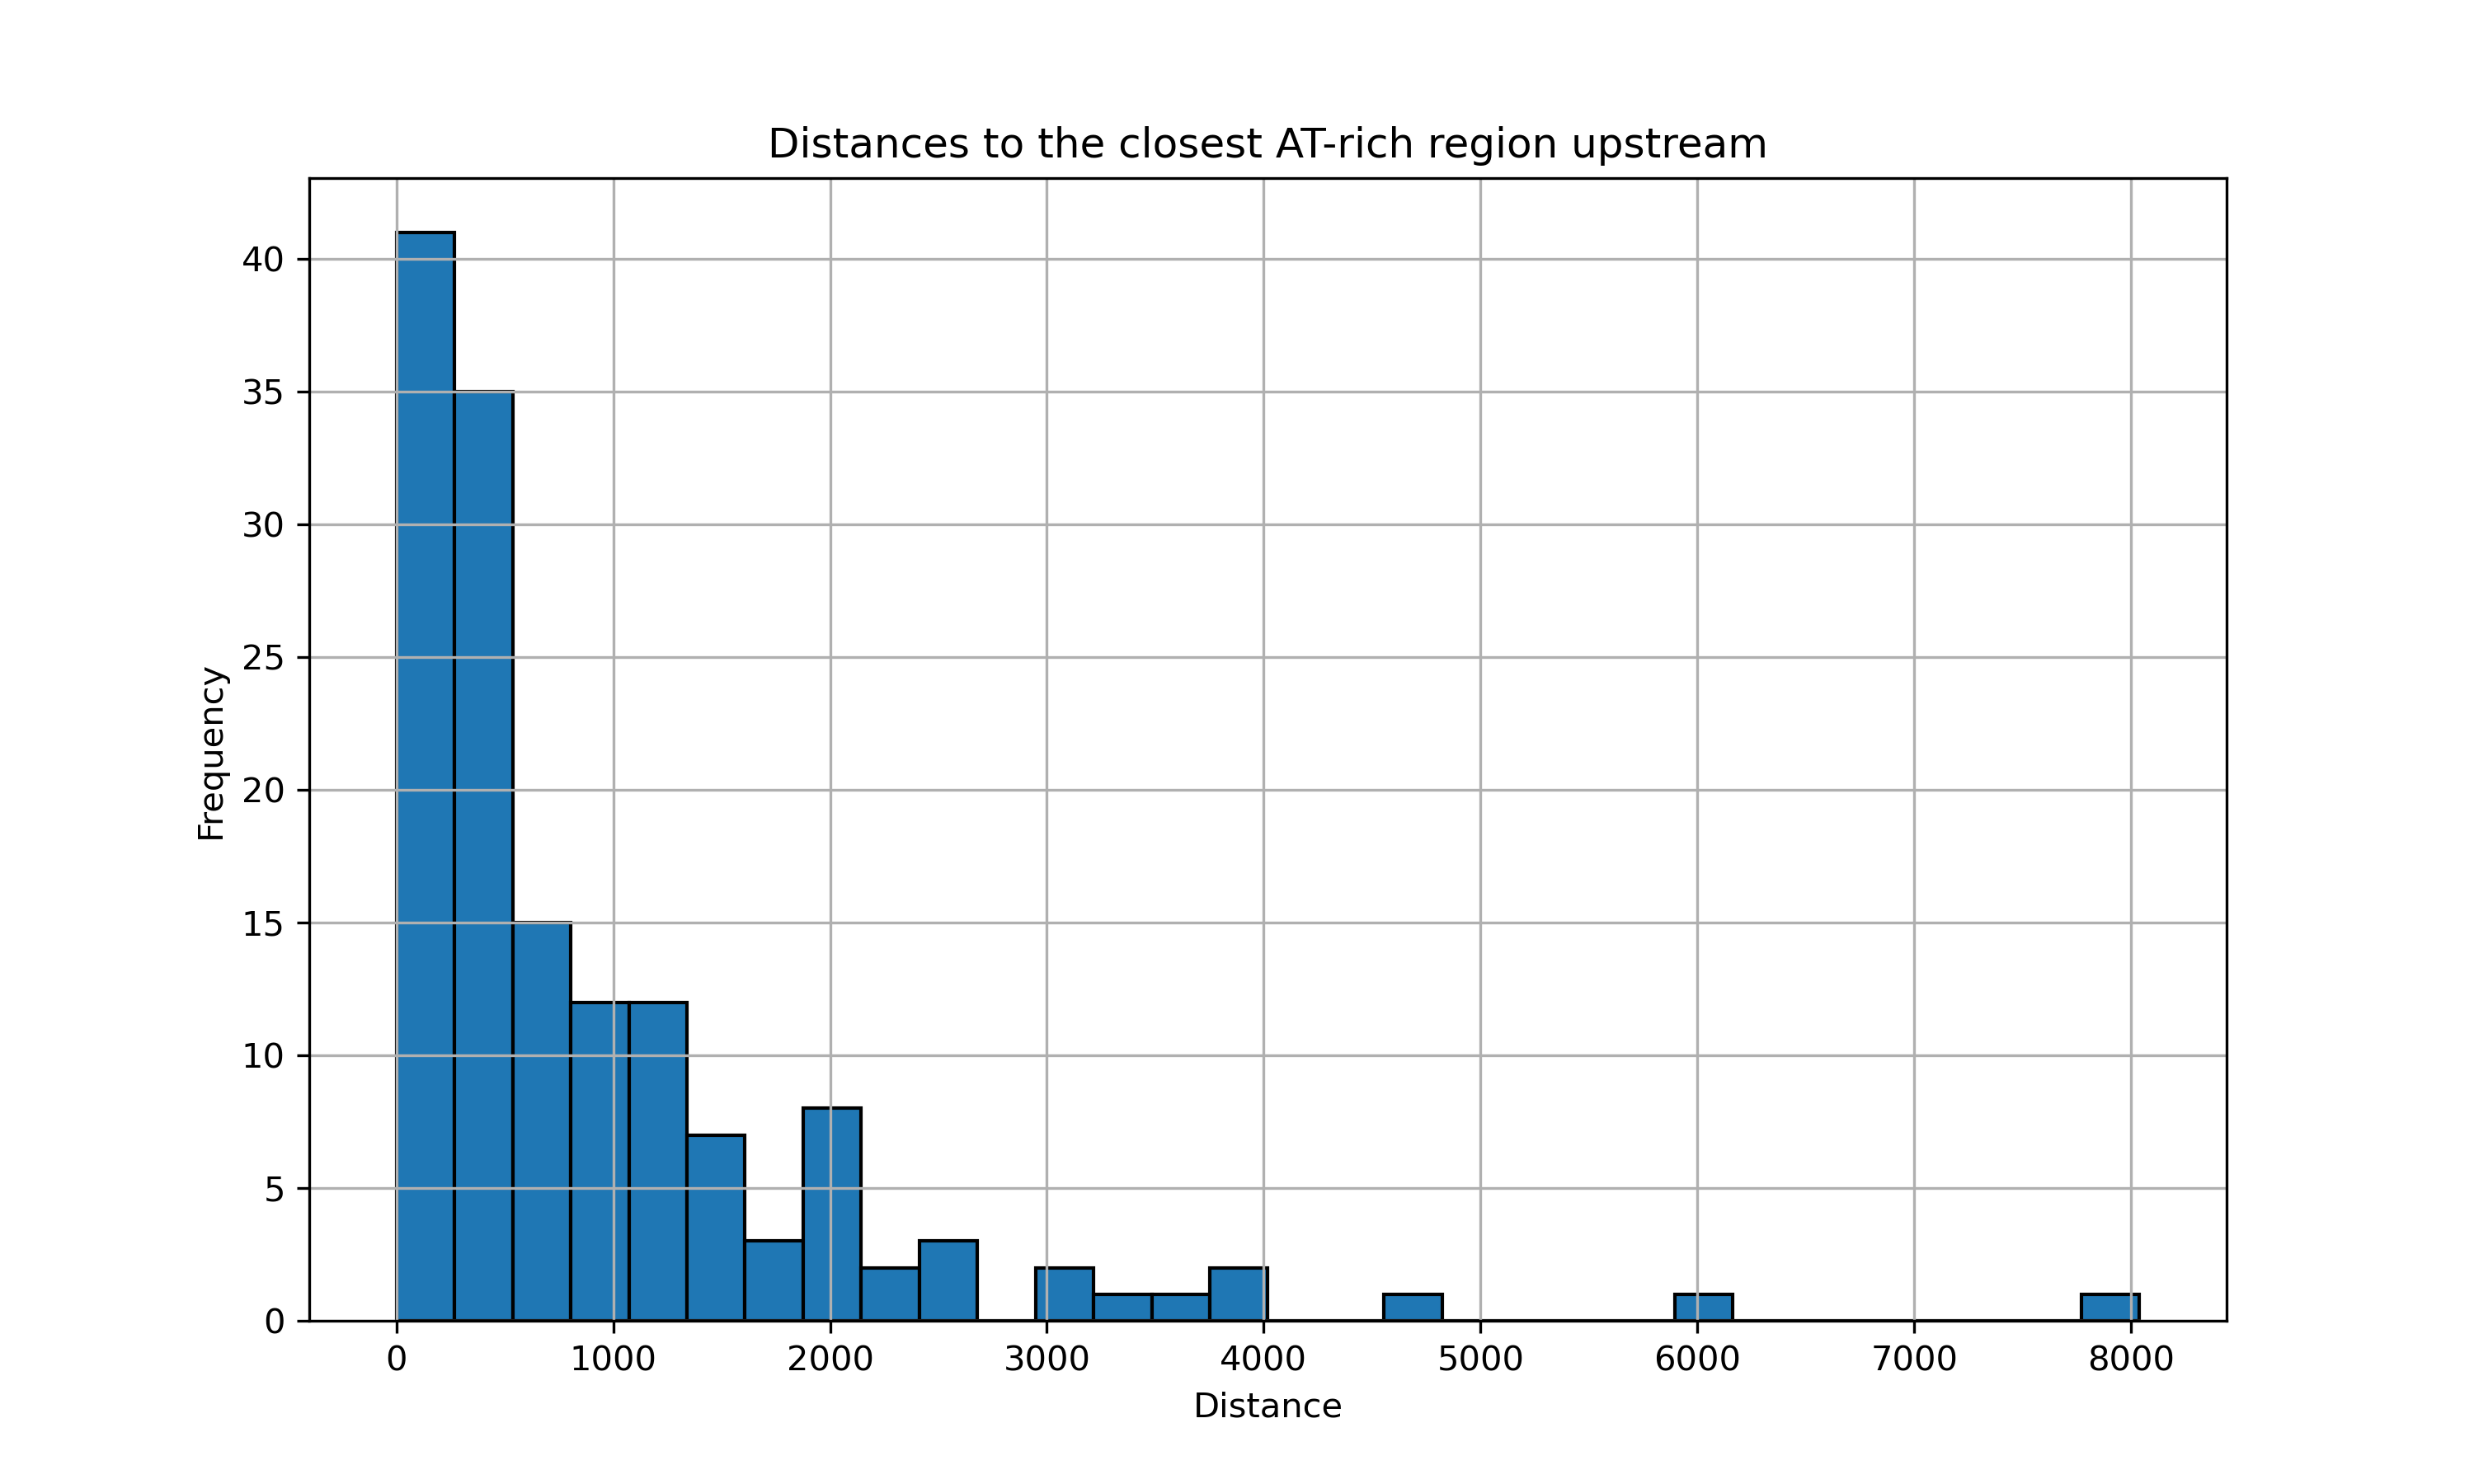
\includegraphics[width=\linewidth]{images/histogramATrich.png}
  \caption{Distances from 3' ends of isolated intergenic regions to closest AT-rich region upstream.}
  \label{fig:distancesATrich}
\end{figure}

\paragraph{Open chromatin}

Open chromatin regions could provide additional evidence of transcriptional activity, if found in the upstream regions.
However, to be more specific, distances to the closest genes should also be found and compared, 
as those open chromatin sites upstream not necessarily are related to our intergenic regions, if there are other genes upstream,
they could be the cause for this.

The distances to open chromatin sites was found for each intergenic regions as well as distances to the closest gene upstream (not strand specific).
Out of 147 isolated intergenic regions, 66 had open chromatin regions closer than any know genes upstream.
However, these could be related to the gene that lay down further upstream,
hence stricter filtering was applied, requiring that the distance between closest open chromatin region and closest gene would be at least 2000bp.
This led to 40 such intergenic regions.

Additionally, if we expect these open chromatin regions to be related to the promoter regions of the isolated intergenic regions,
they also should contain AT-rich regions as described above.
It was checked, and out of the 40 intergenic regions closest open chromatin regions, 38 had AT-rich segment within them.

\paragraph{Conservation scores}

High conservation score of an intergenic region could suggest that it might have some function, i.e. provide additional evidence.
Therefore, a group of possibly biologically meaningful locations were extracted by filtering those genes that have high conservation score
(threshold was set to 0.6) and do not overlap with any known genes (from the ncbi or genecode references). given in the Table \ref{tab:conservedIntergenic}.

\begin{table}[h]
    \centering
    \begin{tabular}{lccc}
        \toprule
        Name & Genomic coordinates & Conservation score & Found in samples \\
        \midrule
        INT1216 & 1:72282700-72282900 & 0.7534172617 & brain, eye\\
	INT1829 & 1:77772950-77773050 & 0.6863111111 & lung \\
	INT2199 & 6:148122550-148122750 & 0.6364459652 & brain, eye \\
	INT2208 & 5:18162950-18163100 & 0.6138651685 & PBMC (indrops) \\
	INT3636 & X:129412750-129413050 & 0.7218984354 & brain \\
        \bottomrule
    \end{tabular}
    \caption{Conserved intergenic regions not overlapping with known genes from ncbi and gencode annotations.}
    \label{tab:conservedIntergenic}
\end{table}


\paragraph{Wrap-up}

\subsection{Antisense intergenic regions}












\iffalse

Firstly, to check if the intergenic regions contain any biologically meaningfull information,
for each sample cells were clustered based only on those intergenic samples.
As can be seen in some provided examples in Figure \ref{fig:intergenicClustering},
clustering can be seen in this case and it roughly corresponds to the clustering using standard ('10x') annotation.
This shows that biologically meaningful information is indeed present in those intergenic regions,
Hence, further analysis were performed on those intergenic regions.

The intergenic regions from all samples were combined into one list, resulting in a list of 13667 entries.
For each region several metrics were calculated, including mean CPM (counts per million) per sample,
the number of samples in which this region was detected, conservation score.
Additionally it was checked if those regions overalap with any genes predicted by gene predictions tools,
also, closest genes on the same and opposite strands (and distances from them) were found.
The list was filtered based on the numer of samples the region was detected, allowing only those regions that are detected in all
blood, brain, eye, or lung samples (with the exception for PBMC samples,
for them more permissive filtering was applied, allowing those entries that were detected only by one sequencing protocol as well,
i.e. it could be detected in all 'PBMC\_10x samples' or all 'PBMC\_indrops samples').
This resulted in a filtered list of 2590 intergenic regions.

Since the filtered list still remained huge, additional filtering criterions were applied:
\begin{itemize}
  \item \textbf{Conservation scores.} Since the conservation scores are not strand specific,
  it makes no sense to filter out directly by the conservation score, because in the case there is other gene on the opposite strand
  of defined region, the high conservation score could be induced by this other gene.
  However, if there are no overlapping genes, high conservation score of an intergenic region could suggest that it might have some function.
  Therefore, a group of possibly biologically meaningful locations were extracted by filtering those genes that have high conservation score
  (threshold was set to 0.6) and do not overlap with any known genes (from the ncbi or genecode references).
  \item \textbf{Gene predictions tools.} There are tools that predict genes based on the genomic sequence.
  Such predictions (if overlapping with defined intergenic regions) would support the claim that
  those (overlapping) intergenic regions are not noise, especially if the intergenic peaks would overlap with 3' ends of predicted genes.
  \item \textbf{Intergenic region specificity.} In the case the reads from specific regions are present only in one cell group,
  the biological origin of these reads are very likelly.
  Such specific regions can be noticed using differential gene expression analysis,
  i.e. checking how gene (or in our case, intergenic region) expression varies between different cell types.
  \item \textbf{ATAC data.} ATAC data can show open chromatin regions, which are typically associated with active transcription.
  If the intergenic regions overlap with open chromatin regions, this could provide additional evidence that reads from this region is not noise.
  \item \textbf{Correlations with nearby genes.} If there exist correlations between the expression of the intergenic regions
  and expression of nearby genes, that could suggest that those regions are not noise and are involved in the same pathways as their neighbours.
\end{itemize}

In the following subsections I will explore genes filtered by those strategies separatelly.

\begin{figure}[htbp]
    \centering
    \begin{subfigure}{0.45\textwidth}
        \centering
        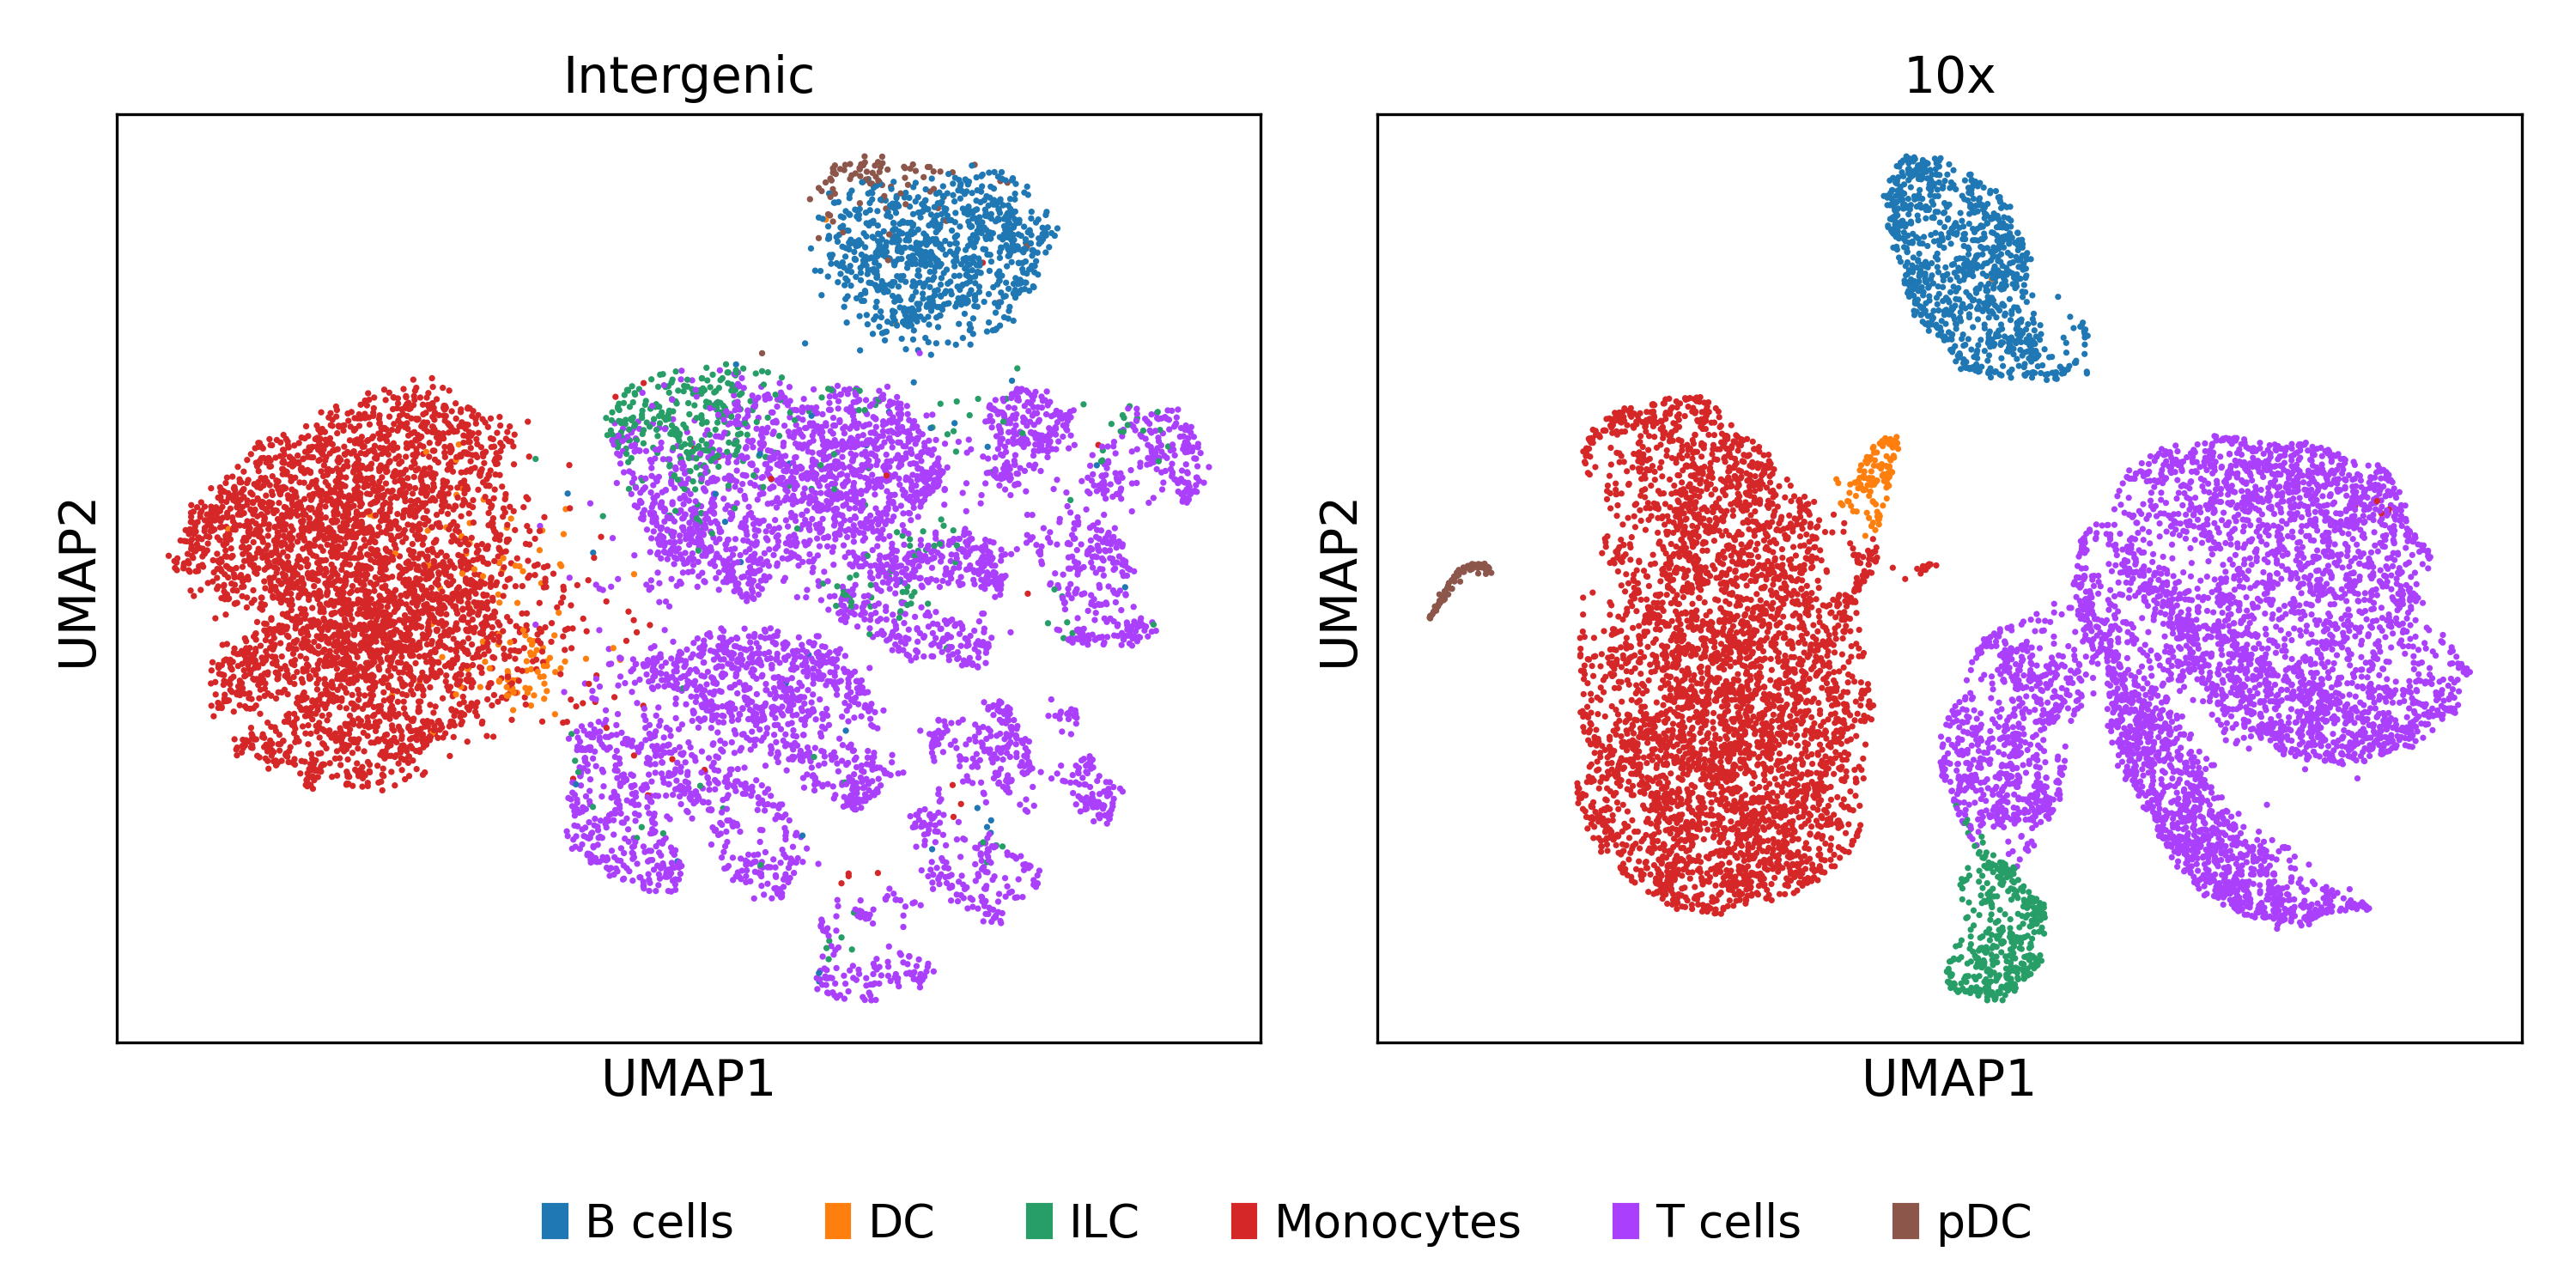
\includegraphics[width=\textwidth]{images/umaps/intergenic_10x_pbmc10x3.png}
        \caption{10x PBMC 3}
    \end{subfigure}
    \hfill
    \begin{subfigure}{0.45\textwidth}
        \centering
        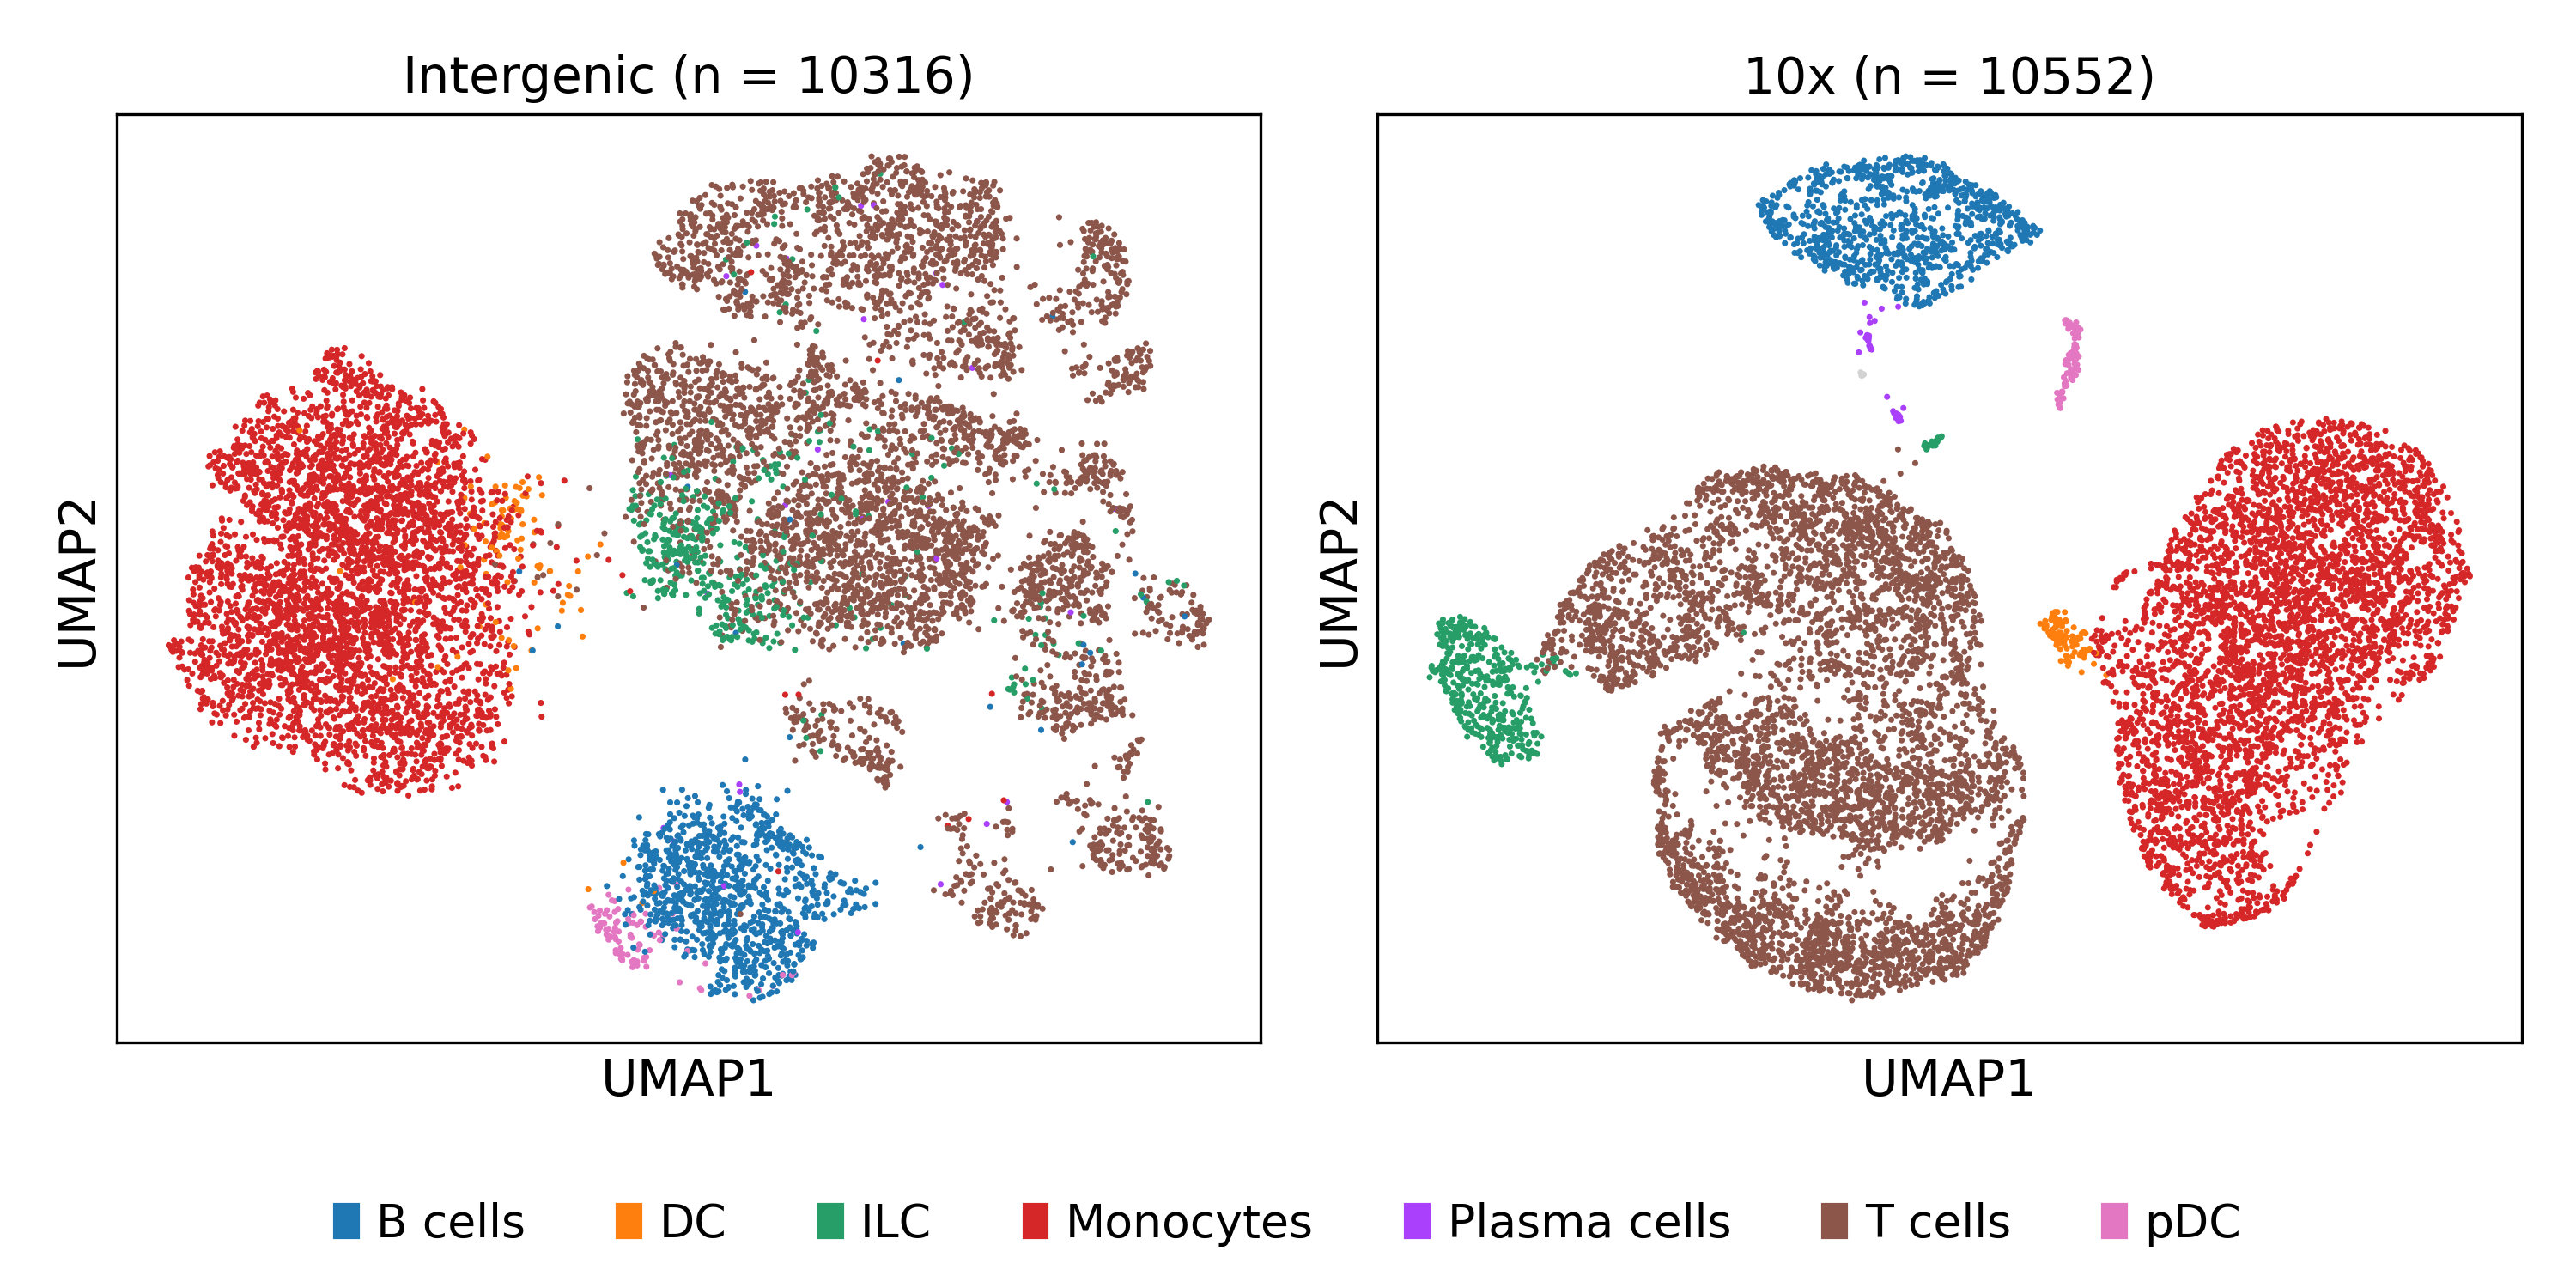
\includegraphics[width=\textwidth]{images/umaps/intergenic_10x_pbmc10x2.png}
        \caption{10x PBMC 2}
    \end{subfigure}
    \vspace{0.5em}
    \begin{subfigure}{0.45\textwidth}
        \centering
        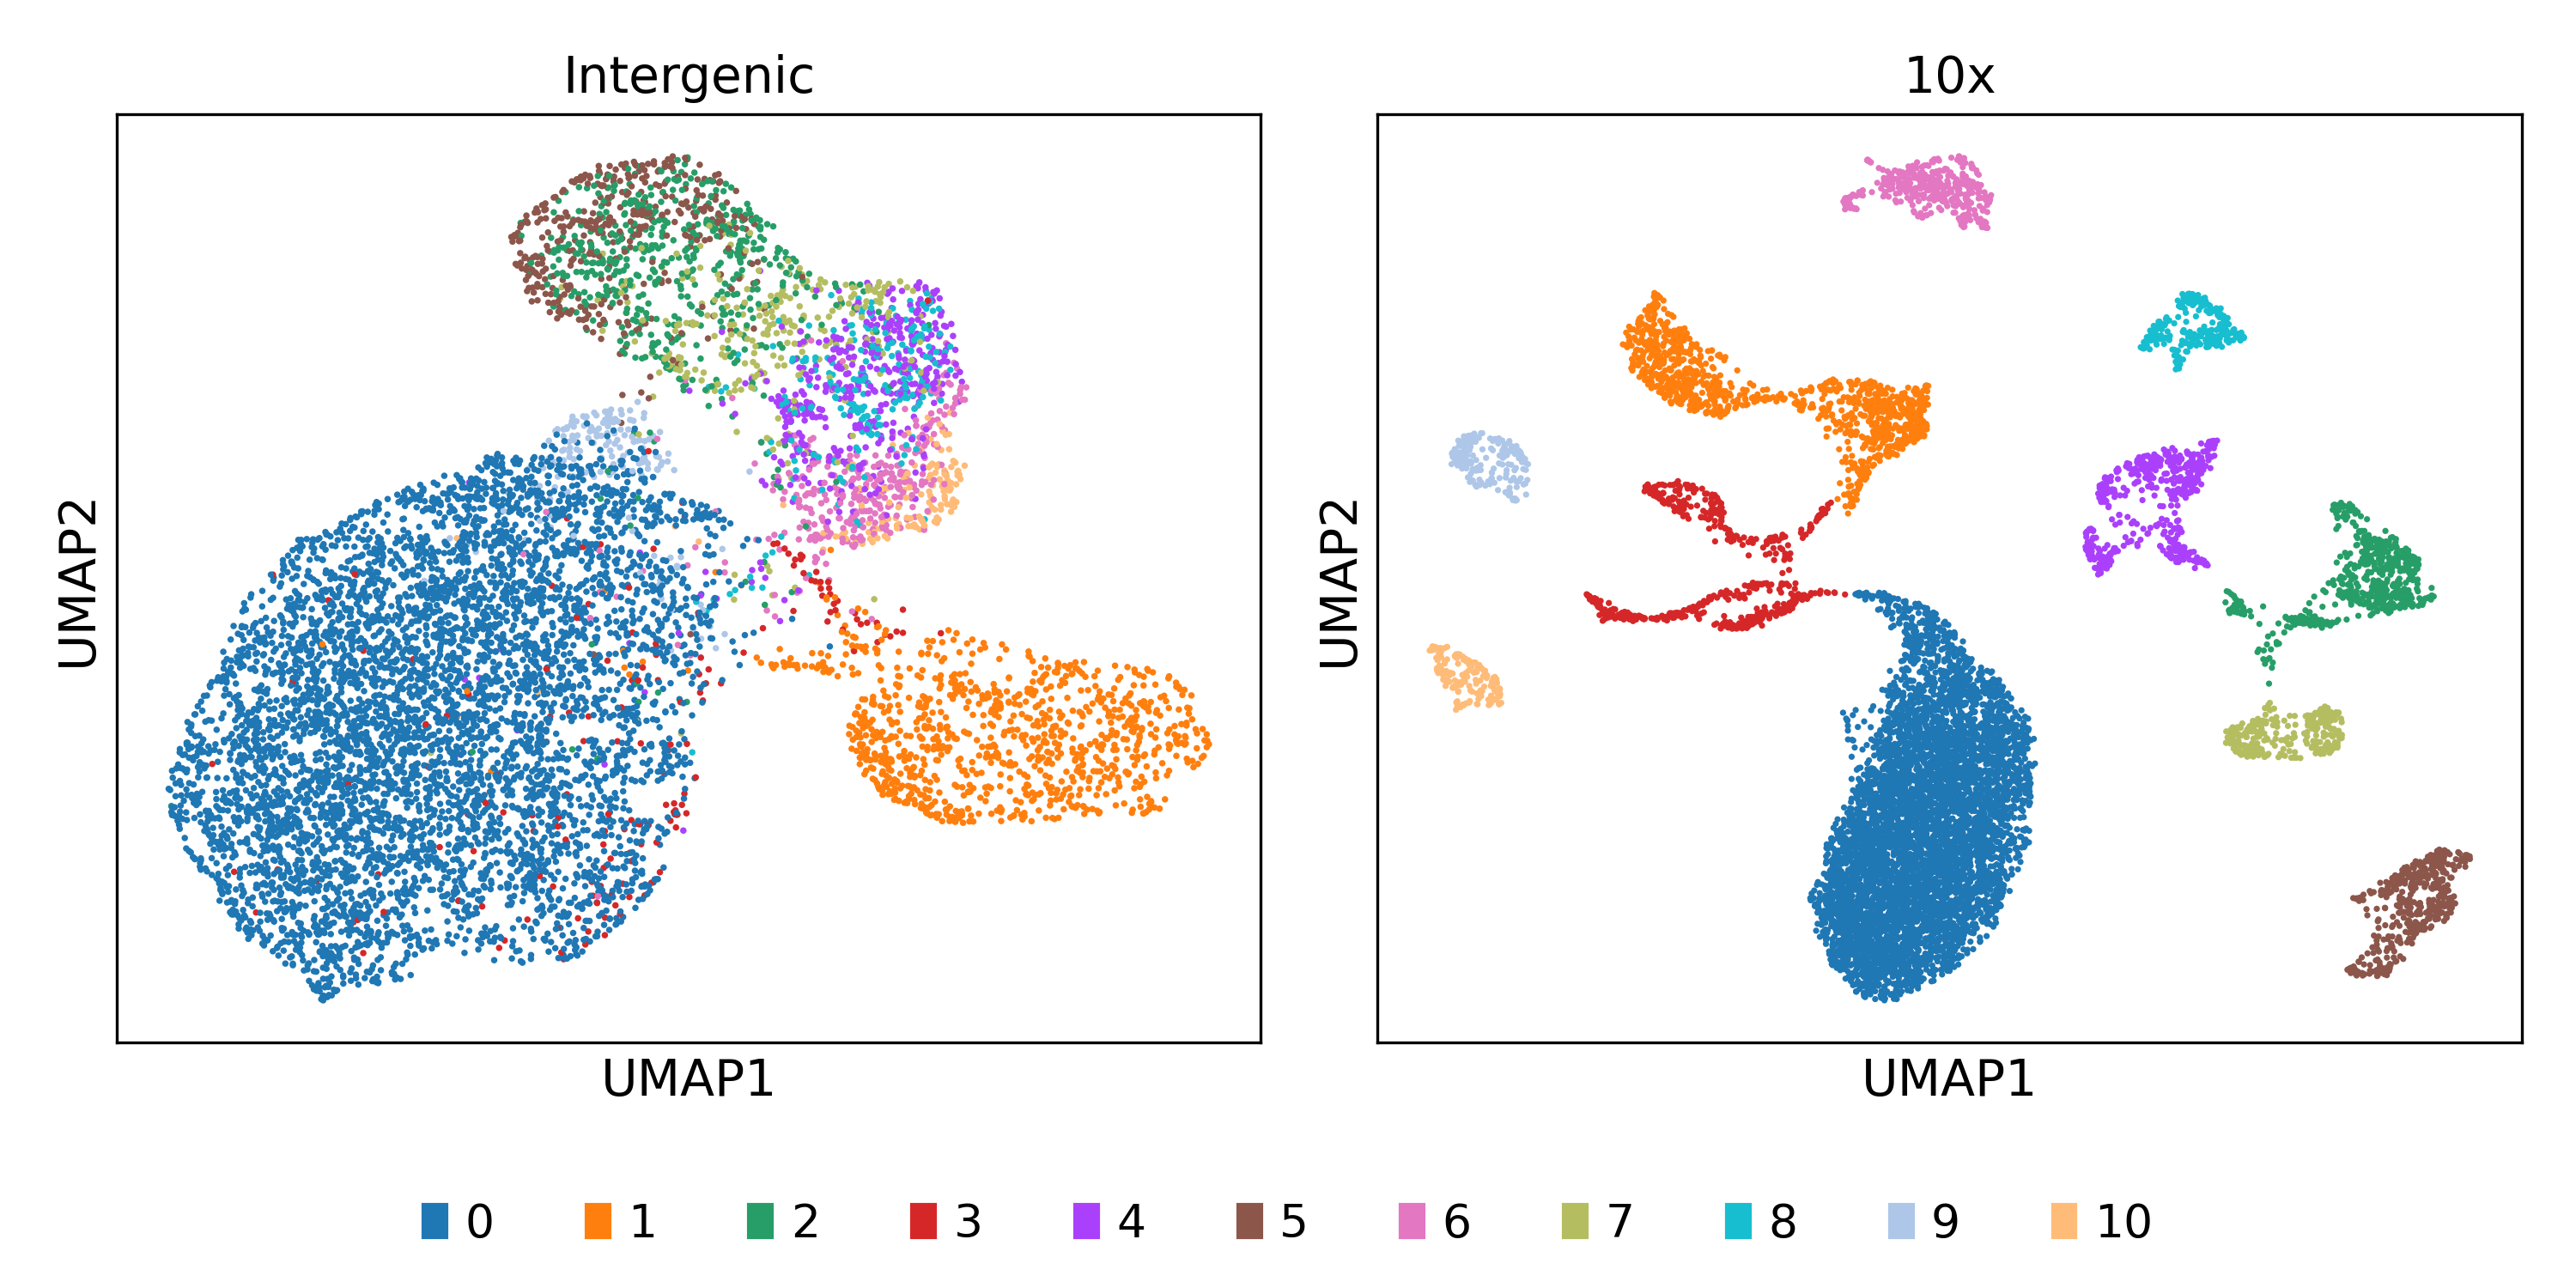
\includegraphics[width=\textwidth]{images/umaps/intergenic_10x_eye.png}
        \caption{eye}
    \end{subfigure}
    \hfill
    \begin{subfigure}{0.45\textwidth}
        \centering
        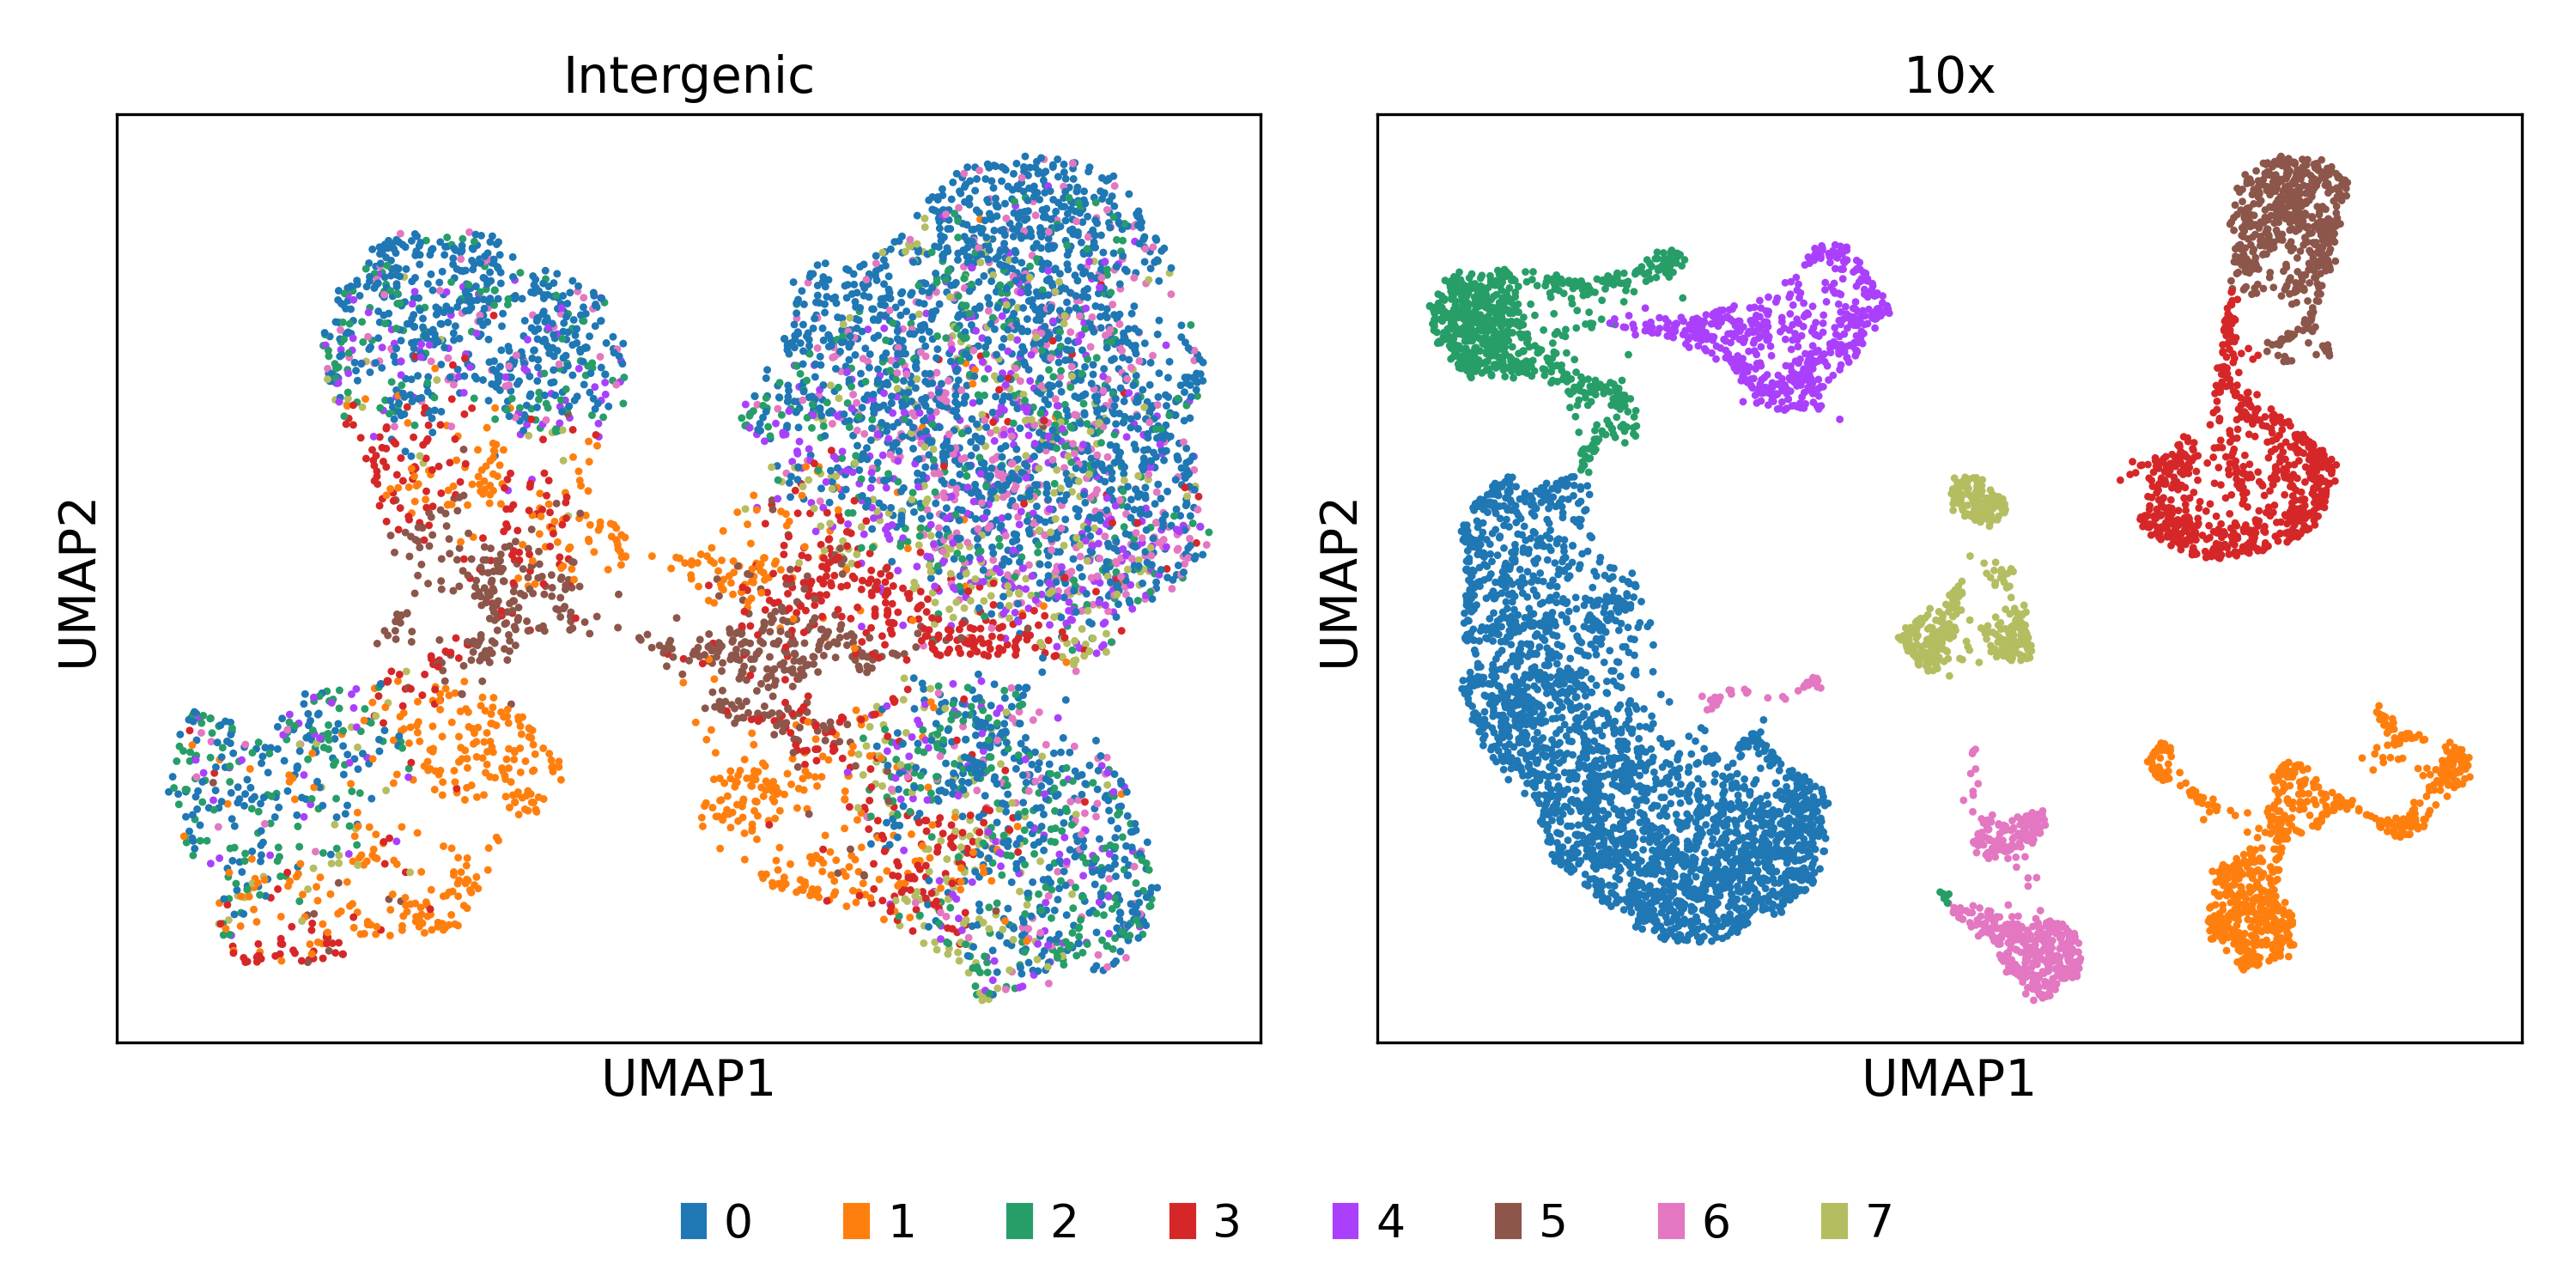
\includegraphics[width=\textwidth]{images/umaps/intergenic_10x_brain_2.png}
        \caption{10x Brain 2}
    \end{subfigure}
    \caption{Comparison of clustering using standard annotation ('10x' reference) and using only defined intergenic regions.
    As can be seen, for some samples intergenic regions are sufficient for rough clustering, for others (e.g. 'brain\_2' sample), 
    noise gives some clustering artefacts.
    Nevertheless, the clustering can be seen even in those noisy samples.}
    \label{fig:intergenicClustering}
\end{figure}

\subsection{Intergenic regions with high conservation score}

The filtering based on the conservation as described above left five intergenic regions, given in the Table \ref{tab:conservedIntergenic}.

\begin{table}[h]
    \centering
    \begin{tabular}{lccc}
        \toprule
        Name & Genomic coordinates & Conservation score & Found in samples \\
        \midrule
        INT1216 & 1:72282700-72282900 & 0.7534172617 & brain, eye\\
	INT1829 & 1:77772950-77773050 & 0.6863111111 & lung \\
	INT2199 & 6:148122550-148122750 & 0.6364459652 & brain, eye \\
	INT2208 & 5:18162950-18163100 & 0.6138651685 & PBMC (indrops) \\
	INT3636 & X:129412750-129413050 & 0.7218984354 & brain \\
        \bottomrule
    \end{tabular}
    \caption{Conserved intergenic regions not overlapping with known genes from ncbi and gencode annotations.}
    \label{tab:conservedIntergenic}
\end{table}

\subsection{Gene Predictions Tools}

61 intergenic regions overlap with predicted genes from UCSC gene prediction archive, given in the Table \ref{tab:predictionToolsIntergenic}.
Of them 44 are in the 3' end of predicted gene (good, as our datasets are generated using 3' end sequencing protocols).
Out of those 44 predicted genes, 15 are extended versions of genes present in gencode/ncbi references,
you can see an example in Figure \ref{fig:predictedExtention}.

\begin{figure}
  \centering
  \includegraphics[width=\linewidth]{images/igv/INT33.png}
  \caption{Example of gene which is predicted to have some longer transcripts than are present in the gencode and ncbi annotations.
  The intergenic region is located after the 3' end of gene DUSP1, however,
  SIB prediction tool suggest that longer transcripts should be included in the annotation of this gene.}
  \label{fig:predictedExtention}
\end{figure}


\begin{table}[h]
    \tiny
    \centering
    \begin{tabular}{lccc}
        \toprule
        Name & Genomic coordinates & Prediction tool & Overlaps with 3' region of predicted gene \\
        \midrule
	INT7 & 6:24718850-24719100 & SIB & Yes \\
	INT33 & 5:172767250-172767500 & SIB & Yes (DUSP1) \\
	INT134 & 15:41280550-41280800 & SIB & Yes (extends a bit after) \\
	INT196 & 6:89086200-89086500 & SIB & Yes (PNRC1) \\
	INT218 & 5:61409150-61409400 & SPG & No (5' end) \\
	INT285 & 10:110898200-110898550 & SIB & Yes (BBIP1) \\
	INT327 & 1:169132100-169132350 & SIB & Yes (NME7) \\
	INT347 & 14:75277700-75278000 & Gescan & No \\
	INT382 & 12:11892250-11892500 & Gescan & Yes \\
	INT386 & 6:26215200-26215450 & SIB & Yes (H2BCB?) \\
	INT438 & 4:39713300-39713600 & SIB & Yes (almost all (short) gene spanned) \\
	INT533 & 8:130110900-130111150 & SIB & Yes \\
	INT617 & 15:85733950-85734200 & SIB & Yes \\
	INT621 & 9:75148850-75149400 & SIB & Yes (OSTF1) \\
	INT651 & 1:28579100-28579350 & SIB & Yes (TRNAU1AP) \\
	INT654 & 6:34382850-34383050 & SIB & No (but short gene)\\
	INT827 & 9:94111950-94112200 & SIB & Yes \\
	INT828 & 8:133035800-133036050 & SIB & Yes (SLA) \\
	INT859 & 2:71373500-71373750 & SIB & No (slight overlap on 5' end) \\
	INT898 & 17:51190400-51190700 & SIB & Yes (extends after)\\
	INT903 & 8:22613400-22613650 & SIB & Yes \\
	INT949 & 9:111693050-111693400 & SIB & Yes \\
	INT972 & 15:64954800-64955350 & SIB & Yes \\
	INT984 & 18:63291900-63292200 & Geneid & Yes No \\
	INT1028 & 5:50414200-50414500 & SIB & Yes No \\
	INT1155 & 1:36296050-36296300 & SIB & Yes No \\
	INT1216 & 1:72282700-72282900 & SIB & Yes No \\
	INT1231 & 10:19890700-19891050 & Gescan & Yes No \\
	INT1387 & 11:63570800-63571050 & SIB & Yes No \\
	INT1402 & 5:142786700-142786950 & SIB & Yes No \\
	INT1440 & 2:235746450-235746700 & SIB & Yes No \\
	INT1445 & 9:40885650-40885900 & SIB & Yes No \\
	INT1525 & 8:11842200-11842350 & SIB & Yes No \\
	INT1548 & 7:50342700-50342950 & Gescan & Yes No \\
	INT1616 & 17:30895450-30895700 & SIB & Yes No \\
	INT1749 & 3:172333550-172333750 & SIB & Yes No \\
	INT1801 & 5:151272550-151272700 & SIB & Yes No \\
	INT1931 & 17:82522100-82522350 & SIB & Yes No \\
	INT2044 & 19:4041150-4041400 & SIB & Yes No \\
	INT2065 & 10:103606150-103606400 & SIB & Yes No \\
	INT2158 & 14:49636100-49636350 & SIB & Yes No \\
	INT2194 & 7:130521250-130521500 & SIB & Yes No \\
	INT2371 & 1:14632650-14632900 & Geneid & Yes No \\
	INT2380 & 22:33853900-33854150 & Geneid & Yes No \\
	INT2825 & 13:45300050-45300300 & Geneid & Yes No \\
	INT2979 & 4:98929350-98929600 & SIB & Yes No \\
	INT3328 & 2:184604250-184604500 & SIB & Yes No \\
	INT3429 & 17:48172750-48173150 & Augustus & Yes No \\
	INT3504 & 15:25332950-25333150 & SIB & Yes No \\
	INT3849 & 3:121432200-121432400 & SIB & Yes No \\
	INT3868 & 17:31448500-31448700 & SIB & Yes No \\
	INT4070 & 4:47430500-47430700 & SIB & Yes No \\
	INT4147 & 1:34861500-34861700 & SIB & Yes No \\
	INT4458 & 5:44820700-44820900 & SIB & Yes No \\
	INT4577 & 5:702050-702300 & SIB & Yes No \\
	INT4743 & 20:3188900-3189050 & SIB & Yes No \\
	INT4948 & 5:703250-703450 & SIB & Yes No \\
	INT5002 & 11:92232750-92232950 & SIB & Yes No \\
	INT5315 & 20:3183750-3184050 & SIB & Yes No \\
	INT5329 & 13:95603000-95603200 & SIB & Yes No \\
	INT5710 & 4:47428500-47428700 & SIB & Yes No \\
        \bottomrule
    \end{tabular}
    \caption{Intergenic regions overlapping with predicted genes from UCSC gene prediction archive.}
    \label{tab:predictionToolsIntergenic}
\end{table}


\subsection{Intergenic regions specific to some cell types}

If reads from specific intergenic region are specific for only subset of cell types present in the sample,
it is strong indication that those reads are not sequencing artefacts.
Examples of such regions can be seen in the Figure \ref{fig:intergenicSpecific}.

\begin{figure}[htbp]
    \centering
    \begin{subfigure}{0.45\textwidth}
        \centering
        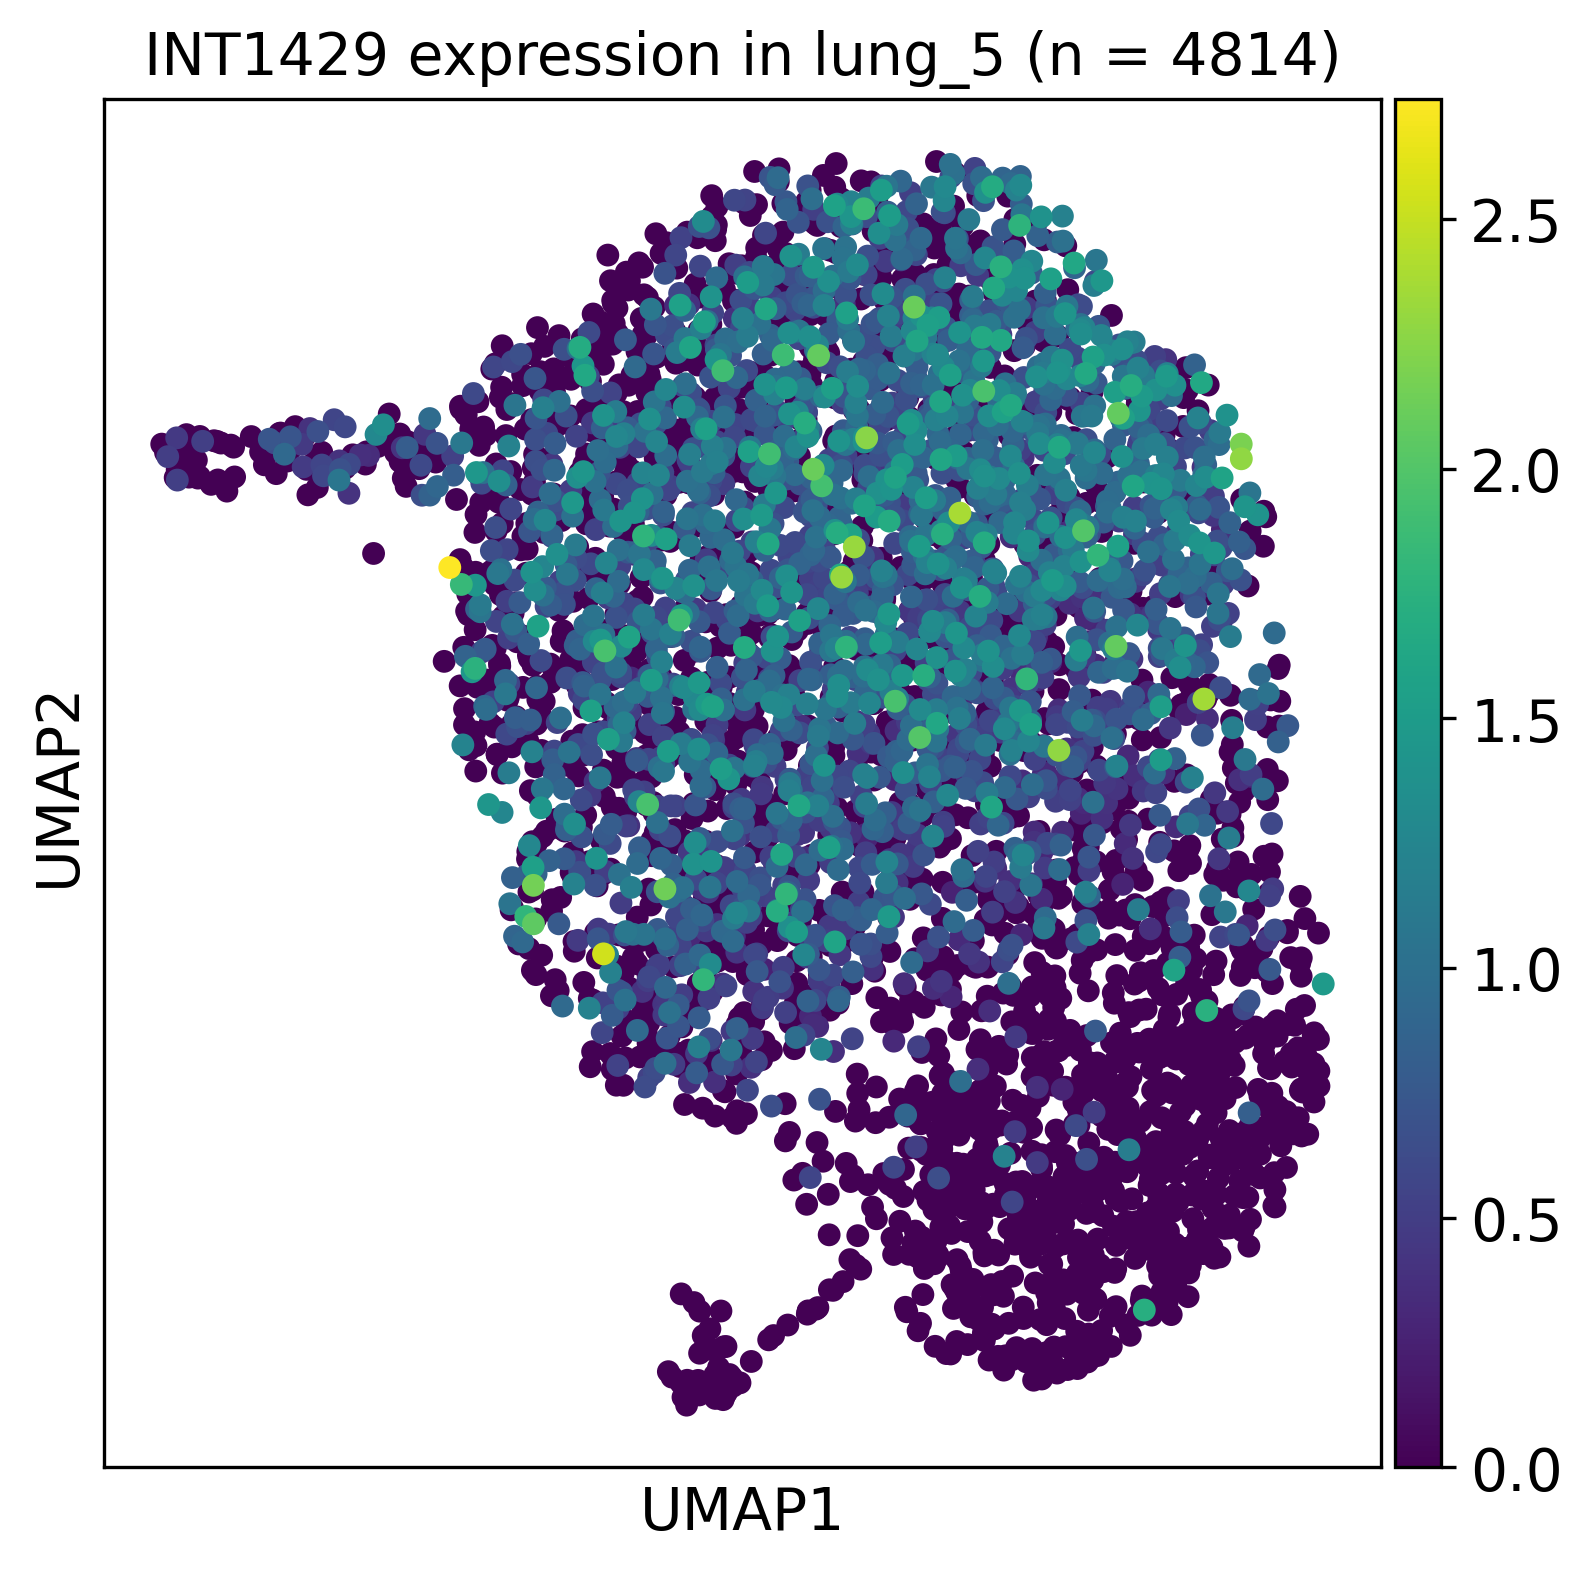
\includegraphics[width=\textwidth]{images/intergenicSpecificExamples/INT1429_lung_5.png}
        \caption{Lung 5 (INT1429)}
    \end{subfigure}
    \hfill
    \begin{subfigure}{0.45\textwidth}
        \centering
        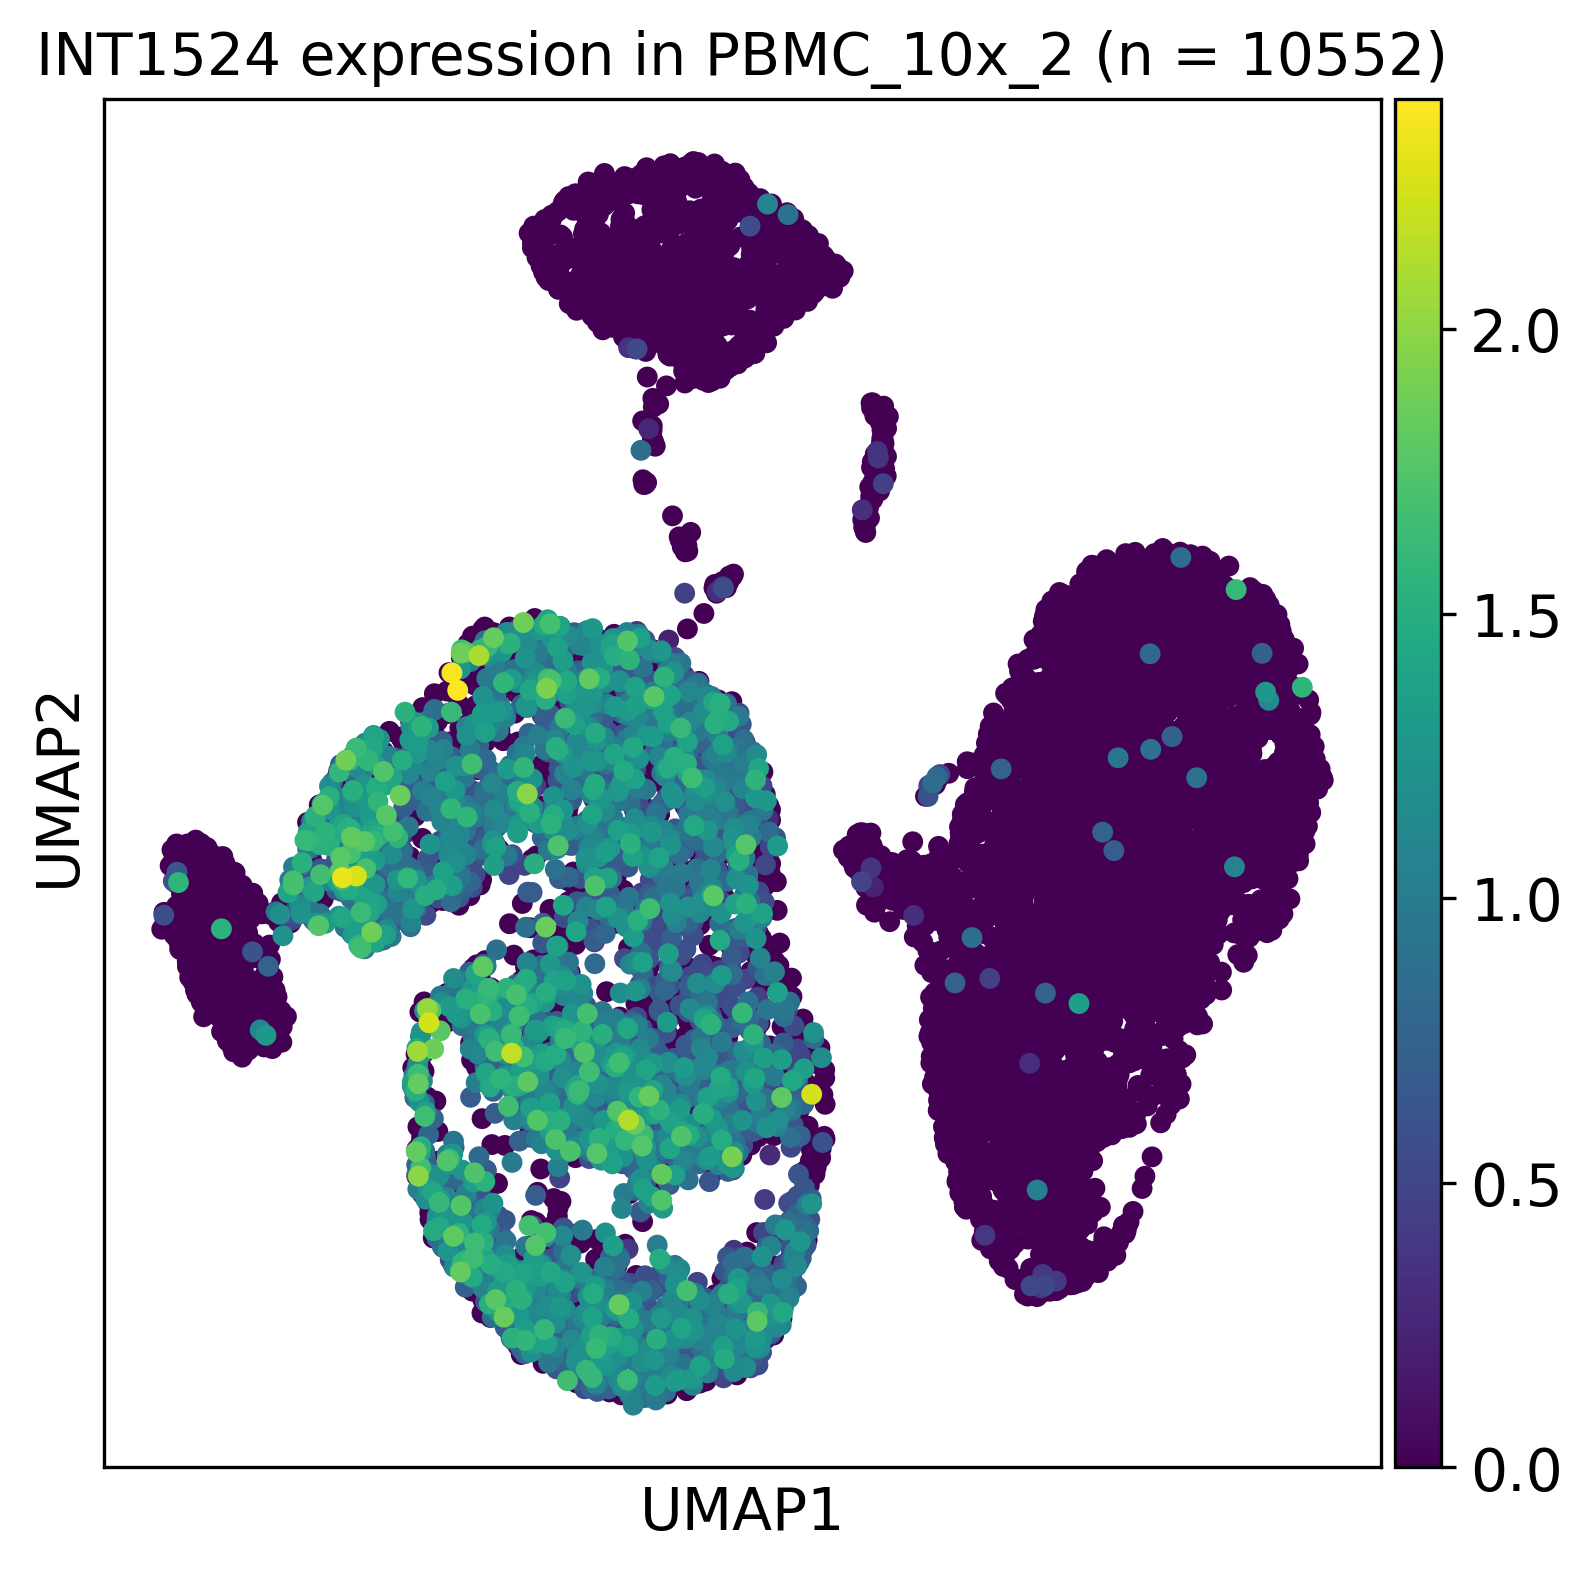
\includegraphics[width=\textwidth]{images/intergenicSpecificExamples/INT1524_PBMC_10x_2.png}
        \caption{PBMC 10x 2 (INT1524)}
    \end{subfigure}
    \vspace{0.5em}
    \begin{subfigure}{0.45\textwidth}
        \centering
        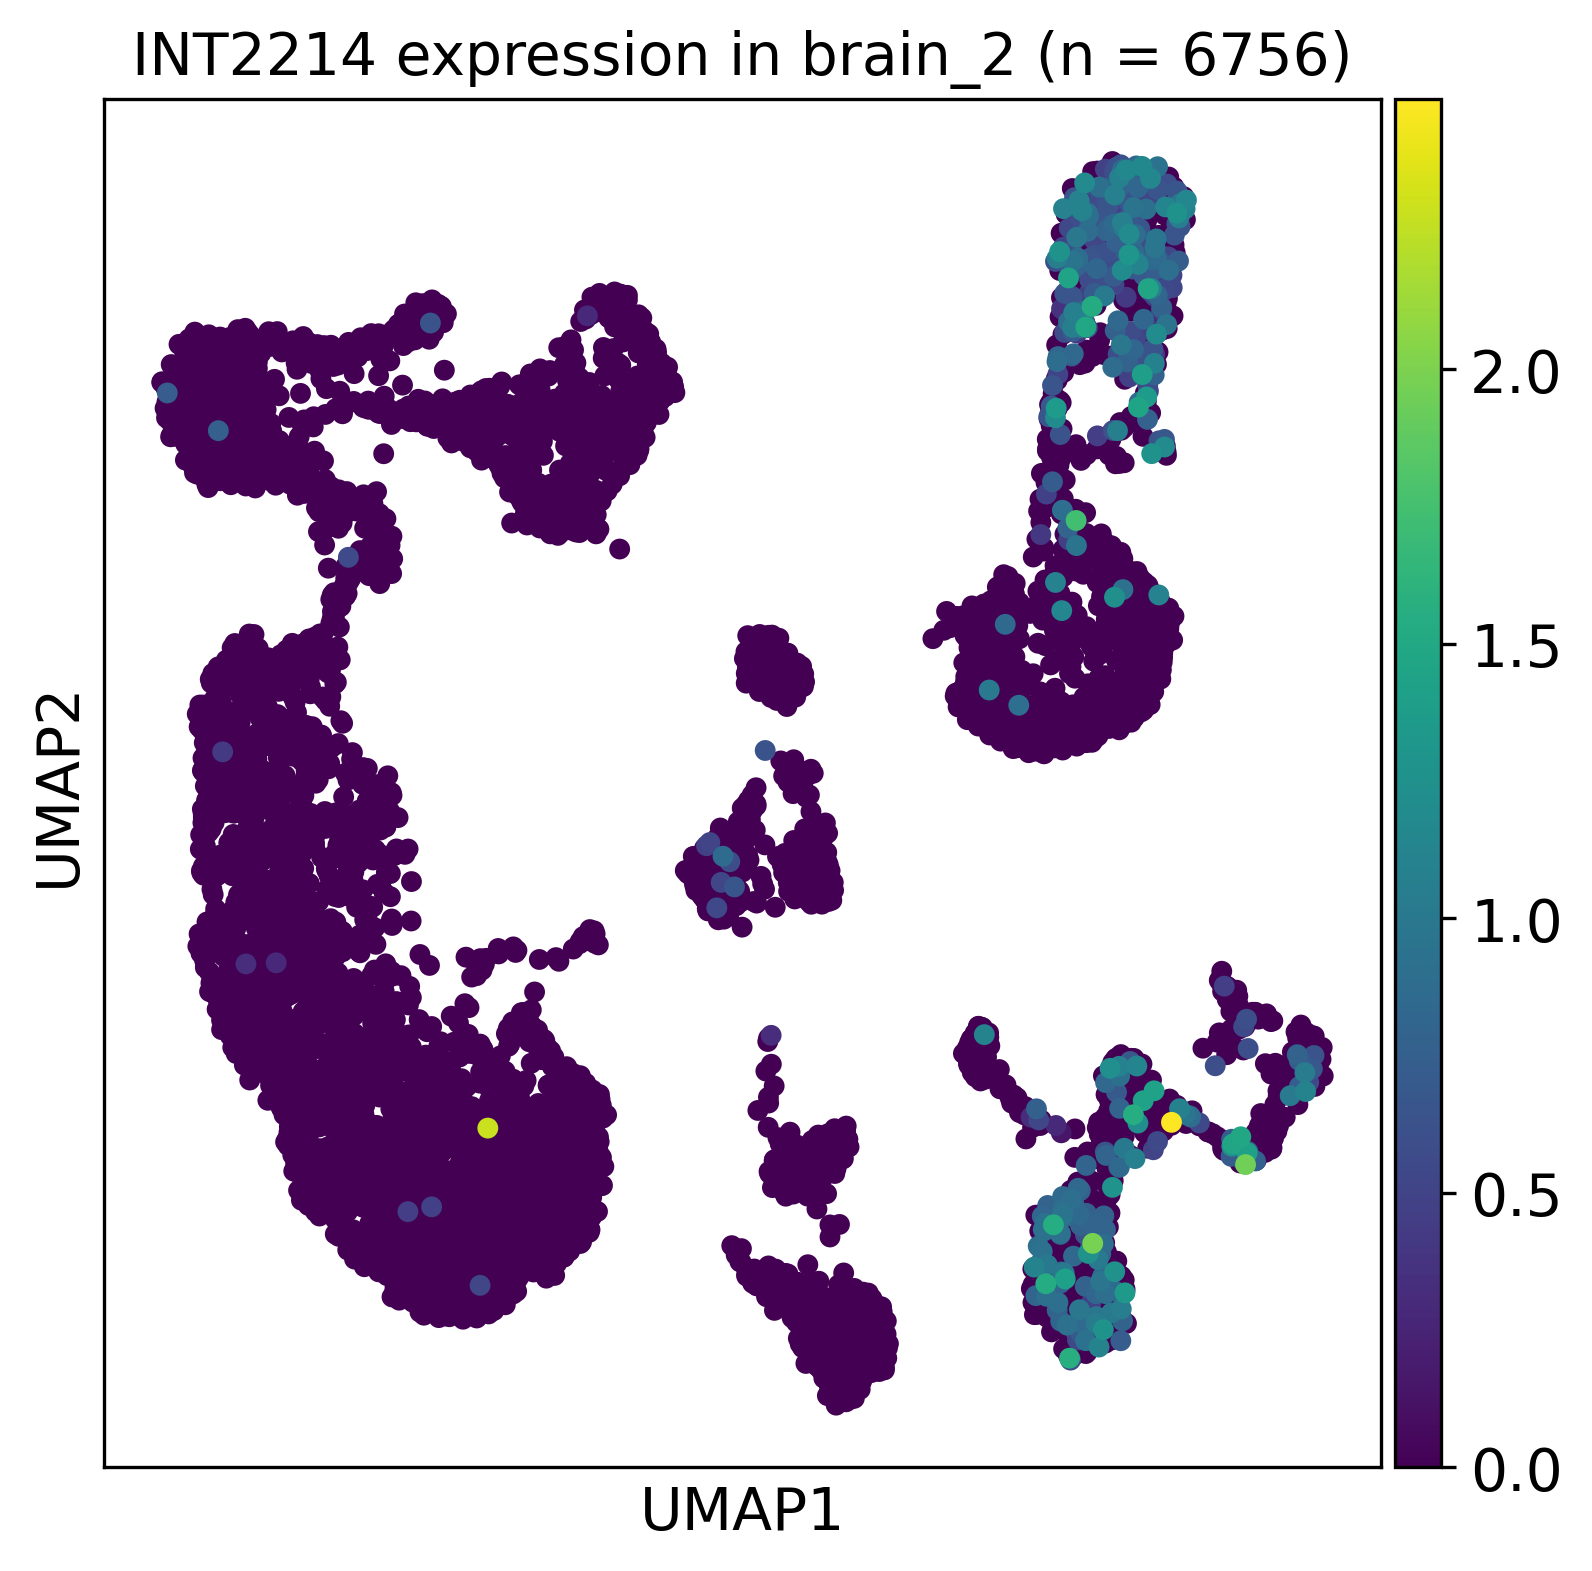
\includegraphics[width=\textwidth]{images/intergenicSpecificExamples/INT2214_brain_2.png}
        \caption{Brain 2 (INT2214)}
    \end{subfigure}
    \hfill
    \begin{subfigure}{0.45\textwidth}
        \centering
        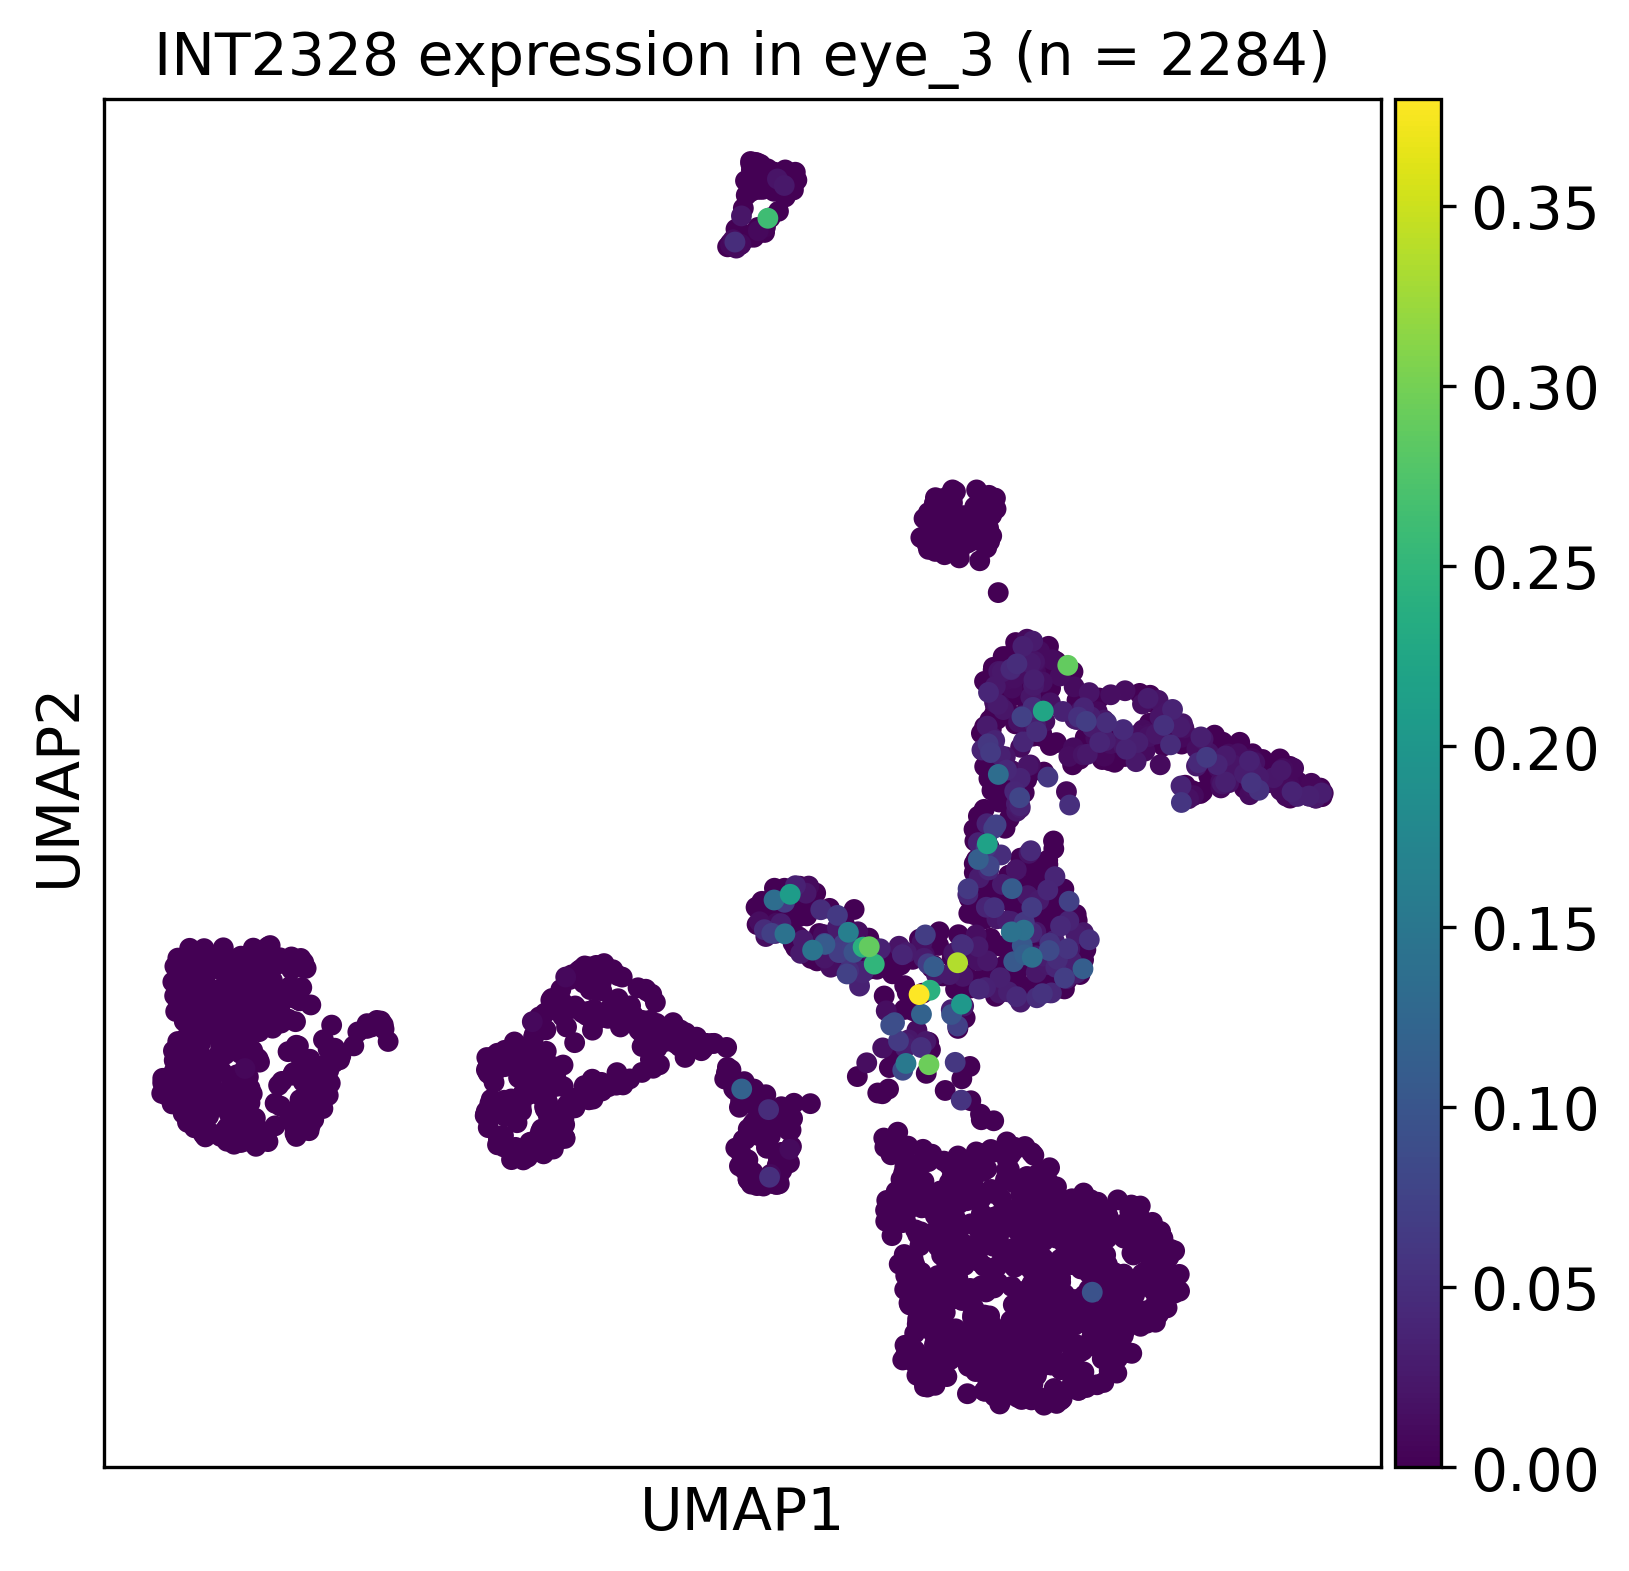
\includegraphics[width=\textwidth]{images/intergenicSpecificExamples/INT2328_eye_3.png}
        \caption{Eye 3 (INT2328)}
    \end{subfigure}
    \caption{Some examples of specificly expressed intergenic regions in various samples.}
    \label{fig:intergenicSpecific}
\end{figure}

\subsection{ATAC data}

ATAC sequencing shows open chromatin sites, which could potentially indicate that some transcription activity is happening at those sites.
Hence, checking if there are overlaps between open chromatine regions and dewfined intergenic regions could provide additional evidence of
those regions being not noise.
However, there are some caveats in this 'evidence'.
Firstly, open chromatin is mostly expected at the transcription start sites, promoter or other regulatory elements,
which are typically located in the 5' end of the gene.
Another problem is that majority of our defined regions lay on the opposite strands of known genes, while ATAC sequencing is not strand specific.
In such cases, open chromatine could be present due to the transcription of those known genes.

Out of 2590 intergenic regions, 309 intersected with ATAC intervals found from 10x PBMC ATAC data.
Out of those 309 regions, only 20 were not overlapping with genes from GENCODE or RefSeq annotations.

\subsection{Correlations}

Another aspect to check is whether expression of those intergenic regions correlate with the expression of nearby genes.
If it does, it might indicate several things:
\begin{itemize}
  \item If the region correlates with gene on the same strand:
  \begin{itemize}
    \item There might exist longer unannotated transcripts that involve those intergenic regions.
    \item The intergenic genes are involved in the same processes as the gene.
    \item They both can be transcribed by the same polymerases.
  \end{itemize}
  \item If the region correlates with gene on the oposite strand:
  \begin{itemize}
    \item The intergenic gene is involved in the same processes as the gene on the oposite strand.
    \item There happens some transcription errors that cause transcription from the opposite strand.
    \item There happens some errors in the library preparation/sequencing steps that cause template switch.
  \end{itemize}
\end{itemize}

Which of those are the case in our samples, is hard to tell.
Out of all defined intergenic regions, 86 showed Spearman correlation \textgreater 0.5 (p \textless 0.05) in at least 1 sample
(80 correlated with genes on the opposite strand, 10 with gene on the same strand, 4 with both).
Some examples can be seen in Figure \ref{fig:correlationUmaps}.

\begin{figure}[htbp]
    \centering
    \begin{subfigure}{\textwidth}
        \centering
        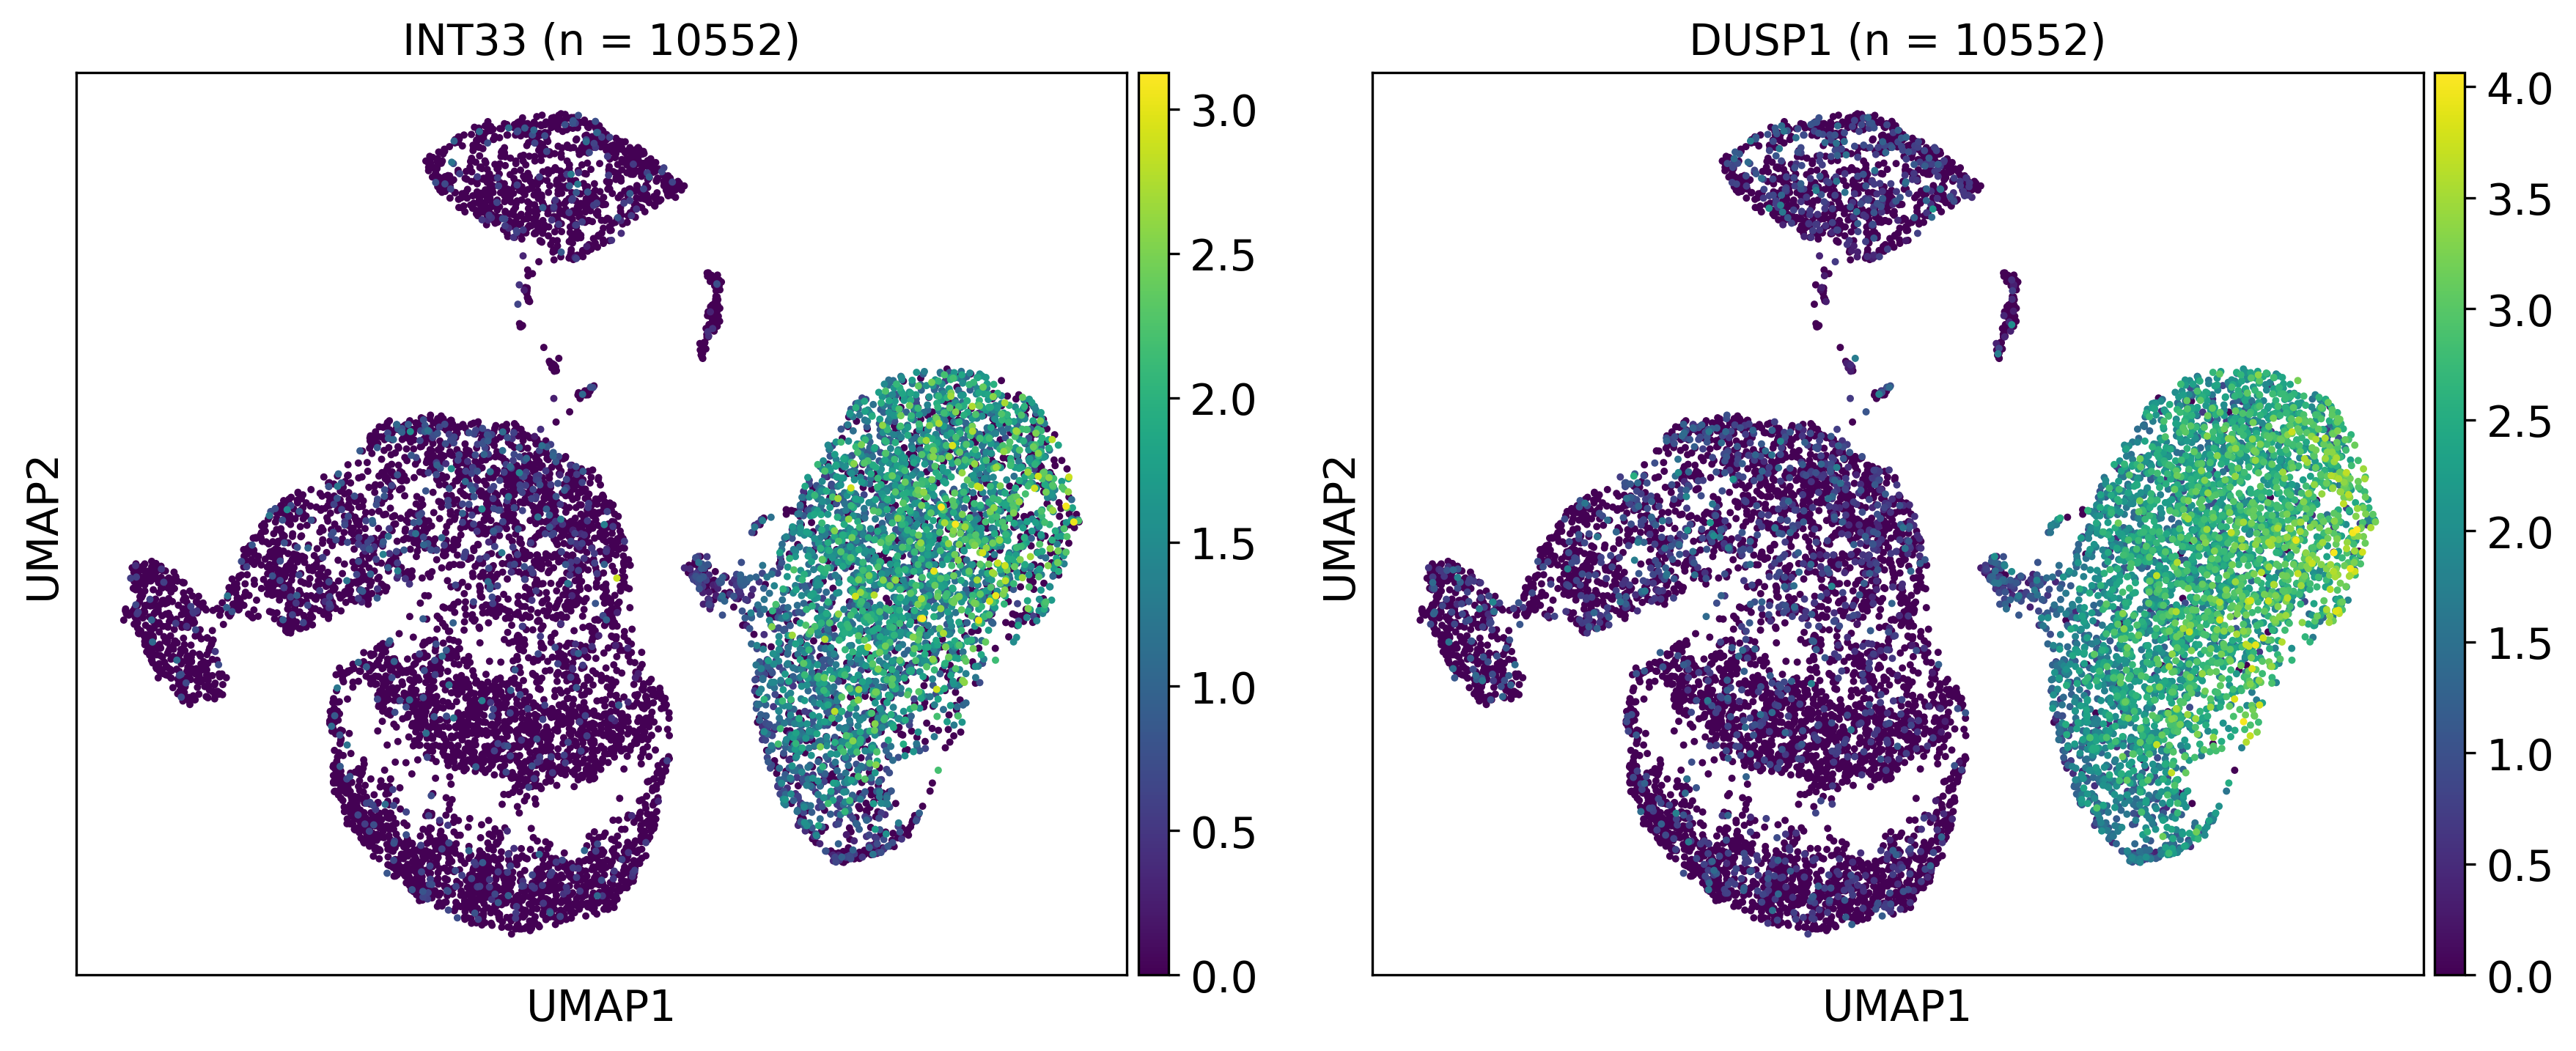
\includegraphics[width=\textwidth]{images/correlationUmaps/PBMC_10x_2_DUSP1.png}
        \caption{Umaps of INT33 and DUSP1 (Spearman correlation 0.68) of the PBMC\_10x\_2 sample, both of them are on the same strand.}
    \end{subfigure}
    \vspace{0.5em}
    \begin{subfigure}{\textwidth}
        \centering
        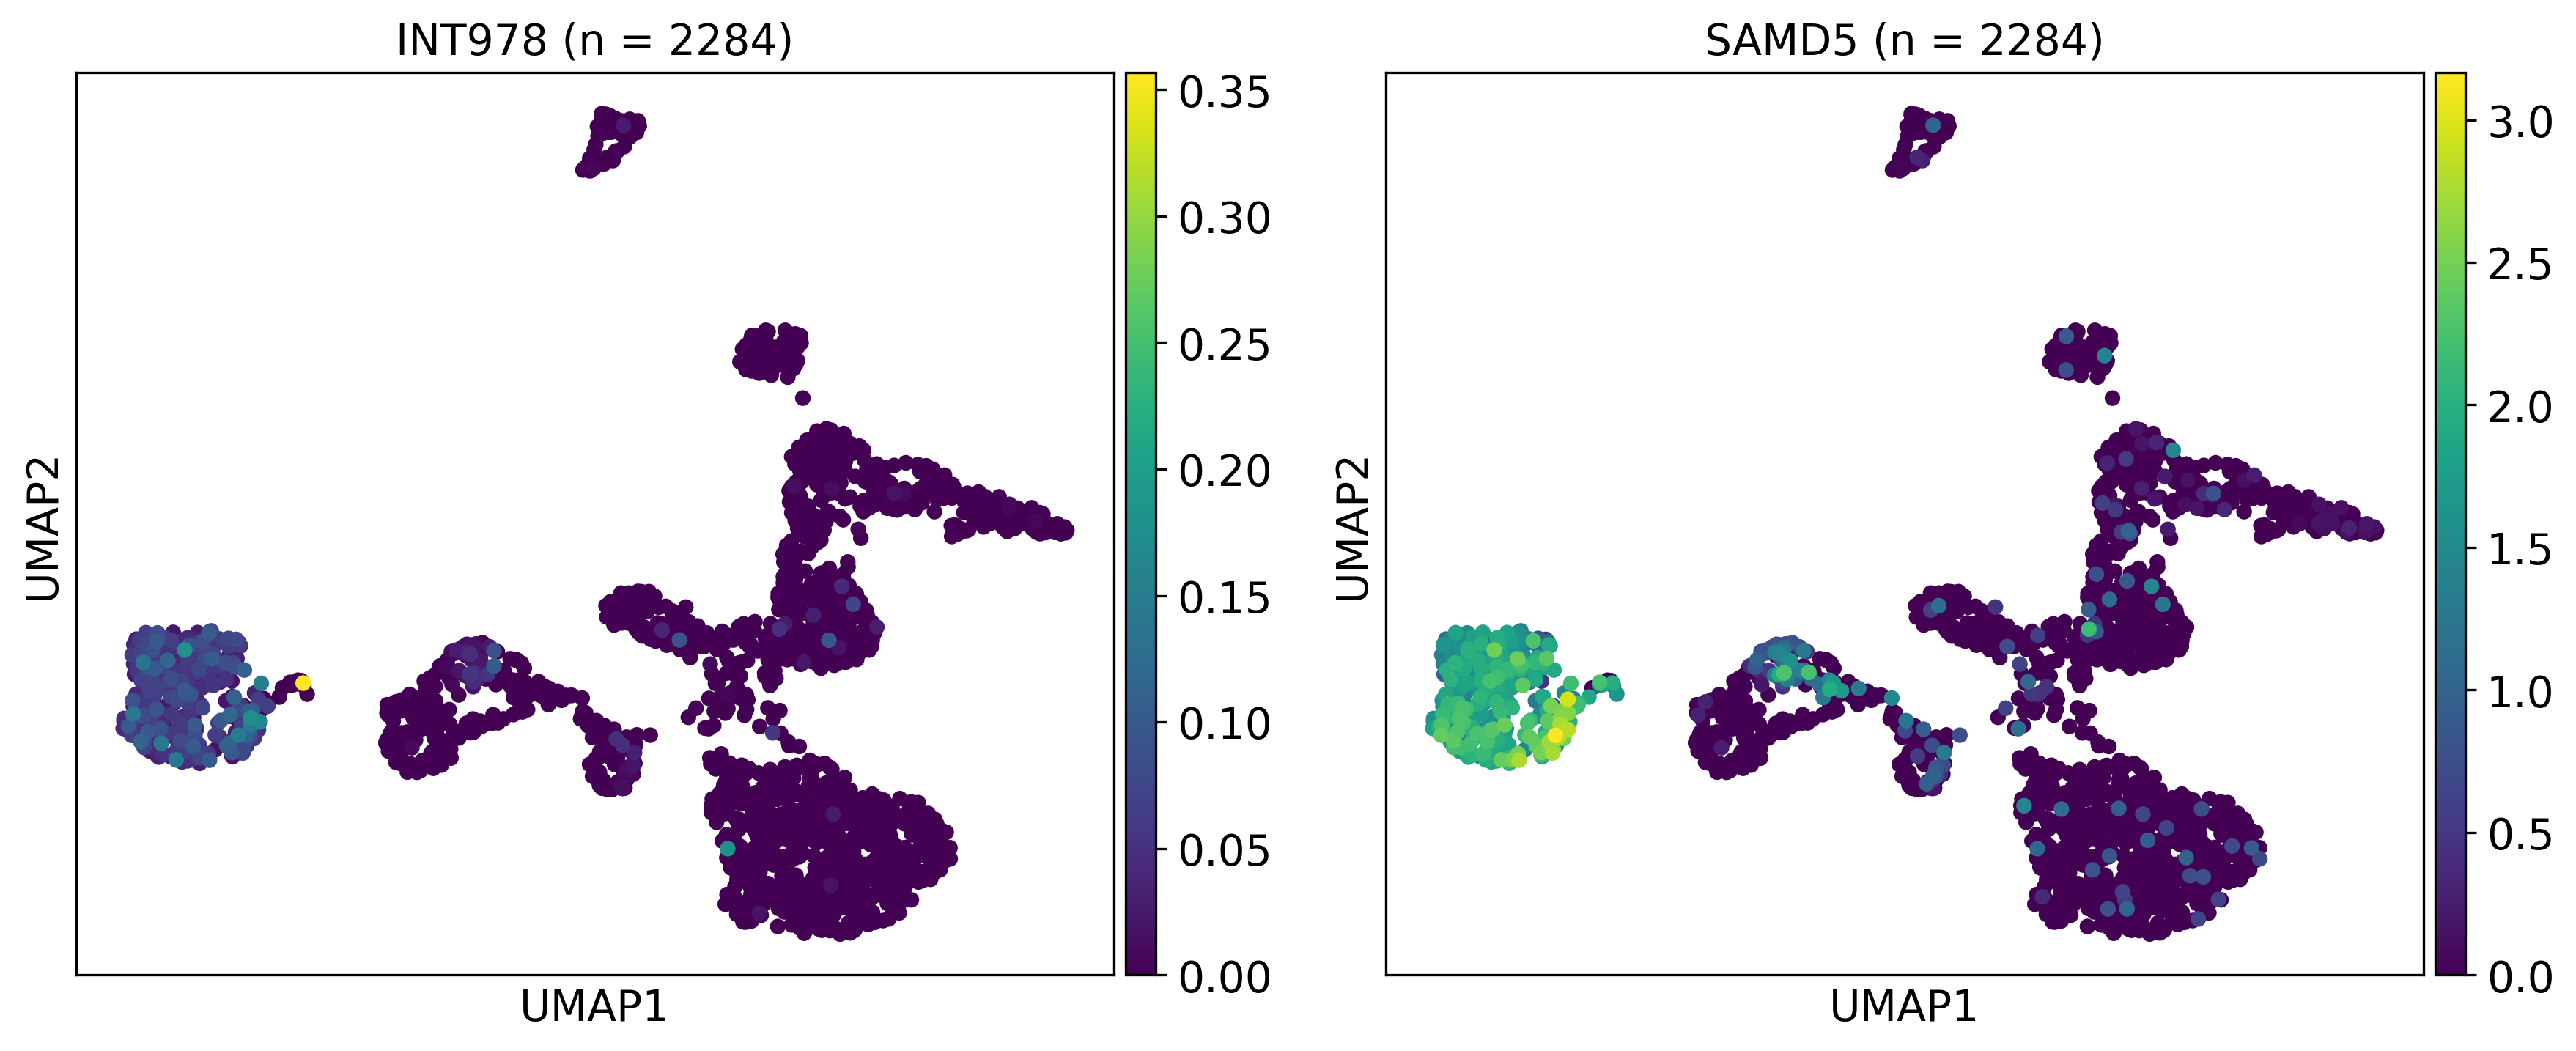
\includegraphics[width=\textwidth]{images/correlationUmaps/eye_3_SAMD5.png}
        \caption{Umaps of INT978 and SAMD5 (Spearman correlation 0.85) of the eye\_3 sample,
        intergenic region is on the opposite strand of the gene.}
    \end{subfigure}
    \caption{Correlation can be seen visually in UMAPs (colored by the normalized expression of the genes), here couple of examples given.}
    \label{fig:correlationUmaps}
\end{figure}

\fi



\iffalse

\section{Enhancing transcriptomic reference}

The enhanced transcriptomic reference allows to include those reads into downstream analysis that otherwise would be discarded.
To achieve this, we have combine data from several different transcriptomic annotations,
and additionally included in the annotation intergenic regions that contained relativelly high number of reads.

\input{"data/downstream/summaries/count_summaries/count_summary.tex"}

\subsection{Exploring unassigned reads}
Unassigned reads could come from several sources:
sequencing artefacts, genes that are not included into transcriptomic reference used, or genes that are not annotated yet.
To check, we have looked at intersections of those unassigned reads and more comprehensive annotations.
As we can see, that there are plenty of genes from more comprehensive annotations which intersect with unassigned genes,
and number of those intersecting genes correlates with sequencing depth.

\input{"data/downstream/summaries/gene_summaries/intersecting_gene_summary.tex"}

\subsection{Intergenic regions}

Observed intergenic regions can be either artefacts or be biologically meaningfull.
To check this, I have tried to cluster cells based only on the newly defined intergenic regions (see figure \ref{fig:umapComparisonIntergenic}).
While for PBMC\_indrops sample it looks as noise, for the 10x indrops samples it provides quite good clustering,
meaning that at least some of those captured intergenic regions are not sequencing artefacts.

\subsection{Enhanced Reference}

Using enhanced reference allowed us to have more captured genes in the data,
however, no significant change in clustering can be seen.

\input{"data/downstream/summaries/captured_gene_summaries/captured_gene_types_summary.tex"}

\subsection{Captured genes}

\fi


\chapter{DISCUSSION}

\chapter{CONCLUSIONS}

\chapter{RECOMMENDATION}

\chapter{ACKNOWLEDGEMENTS}

\chapter{REFERENCES}
\printbibliography[heading=none]

\chapter{SUMMARY}

\chapter{SUMMARY IN LITHUANIAN}

\chapter{APPENDICES}
\begin{figure}[htbp]
\centering
\caption{Clusterings of datasets. 'n' stands for number of cells in the plot, 'res' for the resolution parameter of leiden algorithm.
\textit{PBMC\_10x} samples are colored by CellTypist annotations.}
\label{fig:clusterings}
\begin{tabular}{ccc}
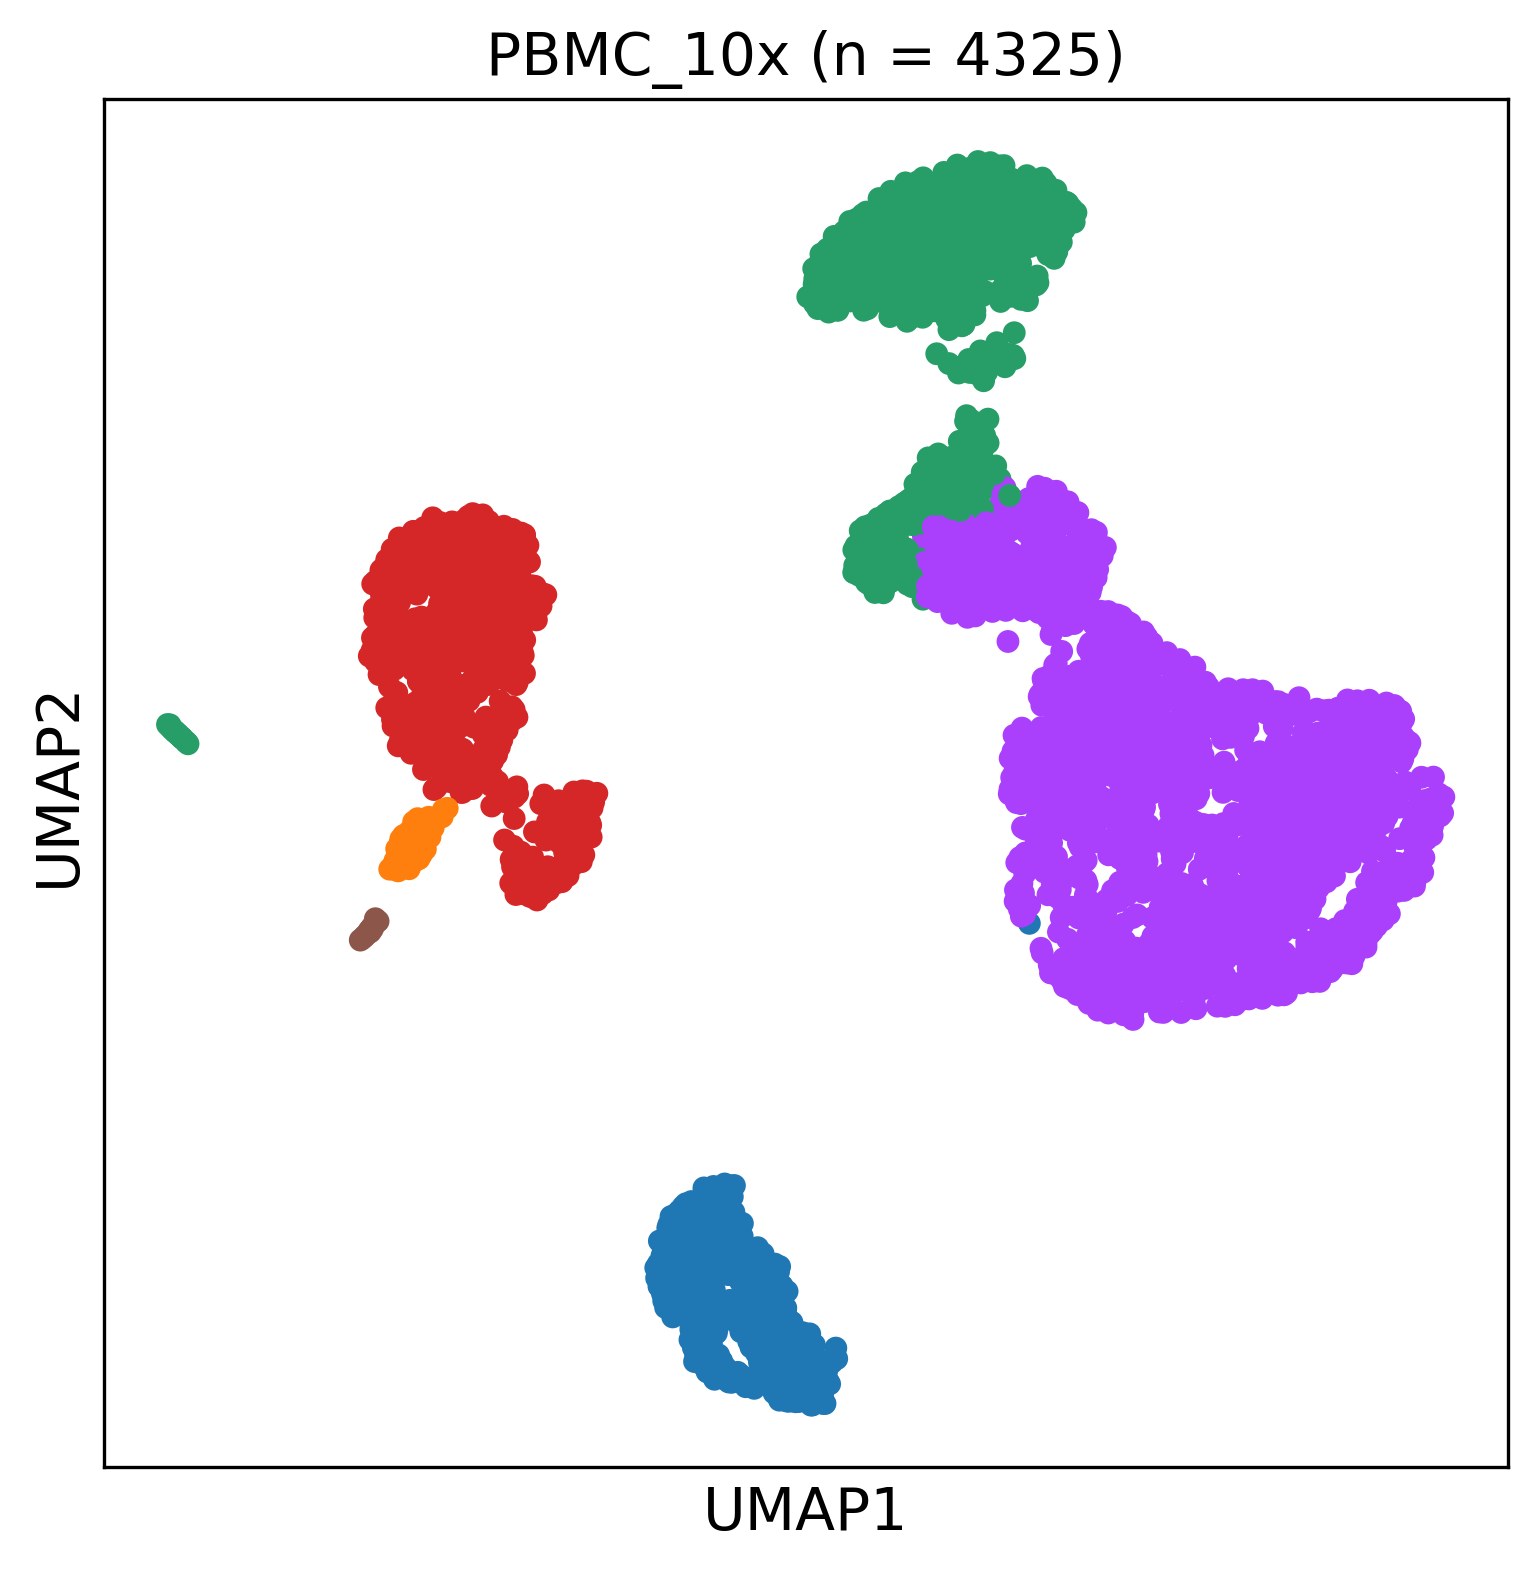
\includegraphics[width=0.25\textwidth]{images/clusterings/PBMC_10x.png} &
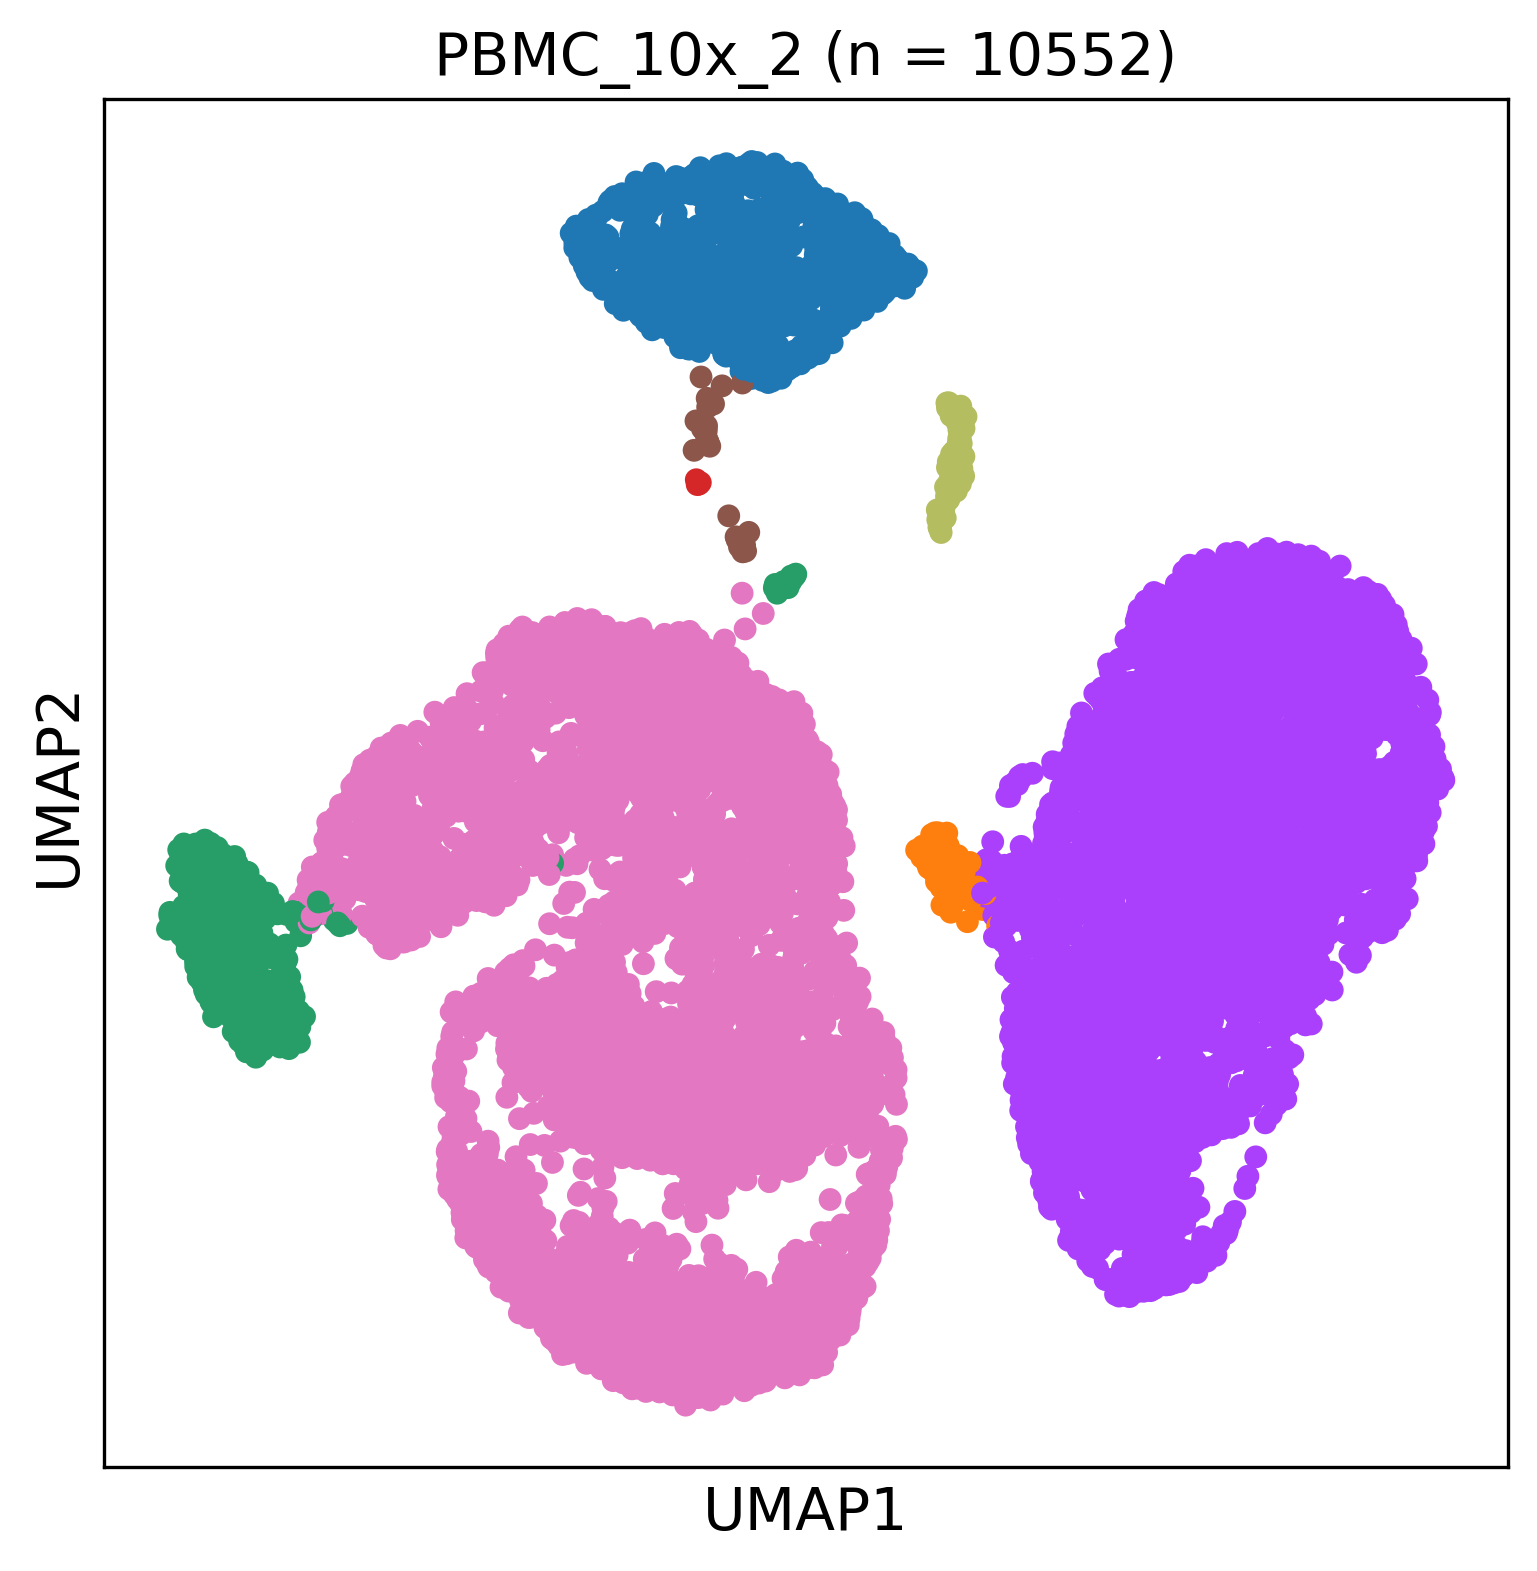
\includegraphics[width=0.25\textwidth]{images/clusterings/PBMC_10x_2.png} &
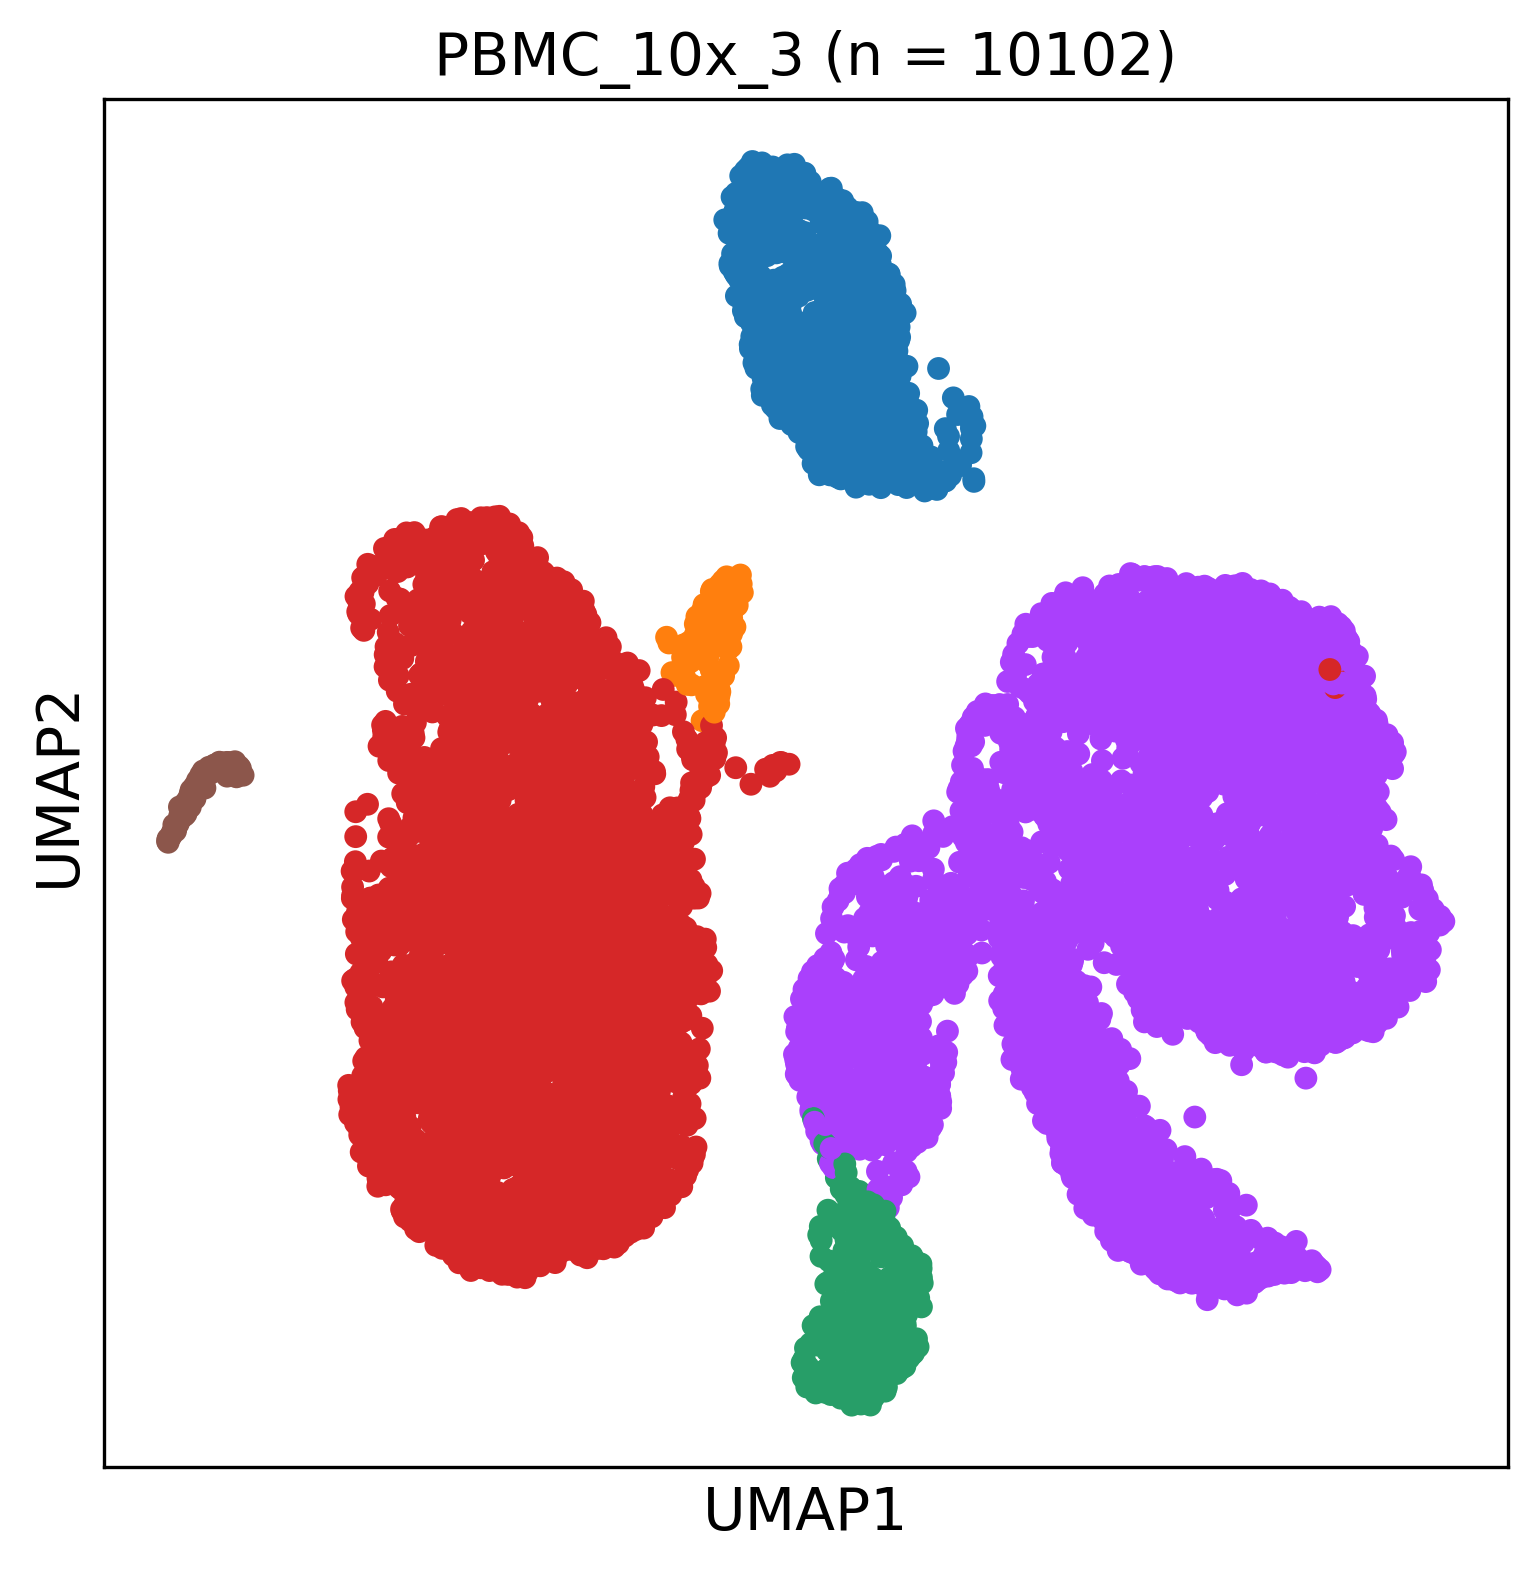
\includegraphics[width=0.25\textwidth]{images/clusterings/PBMC_10x_3.png} \\
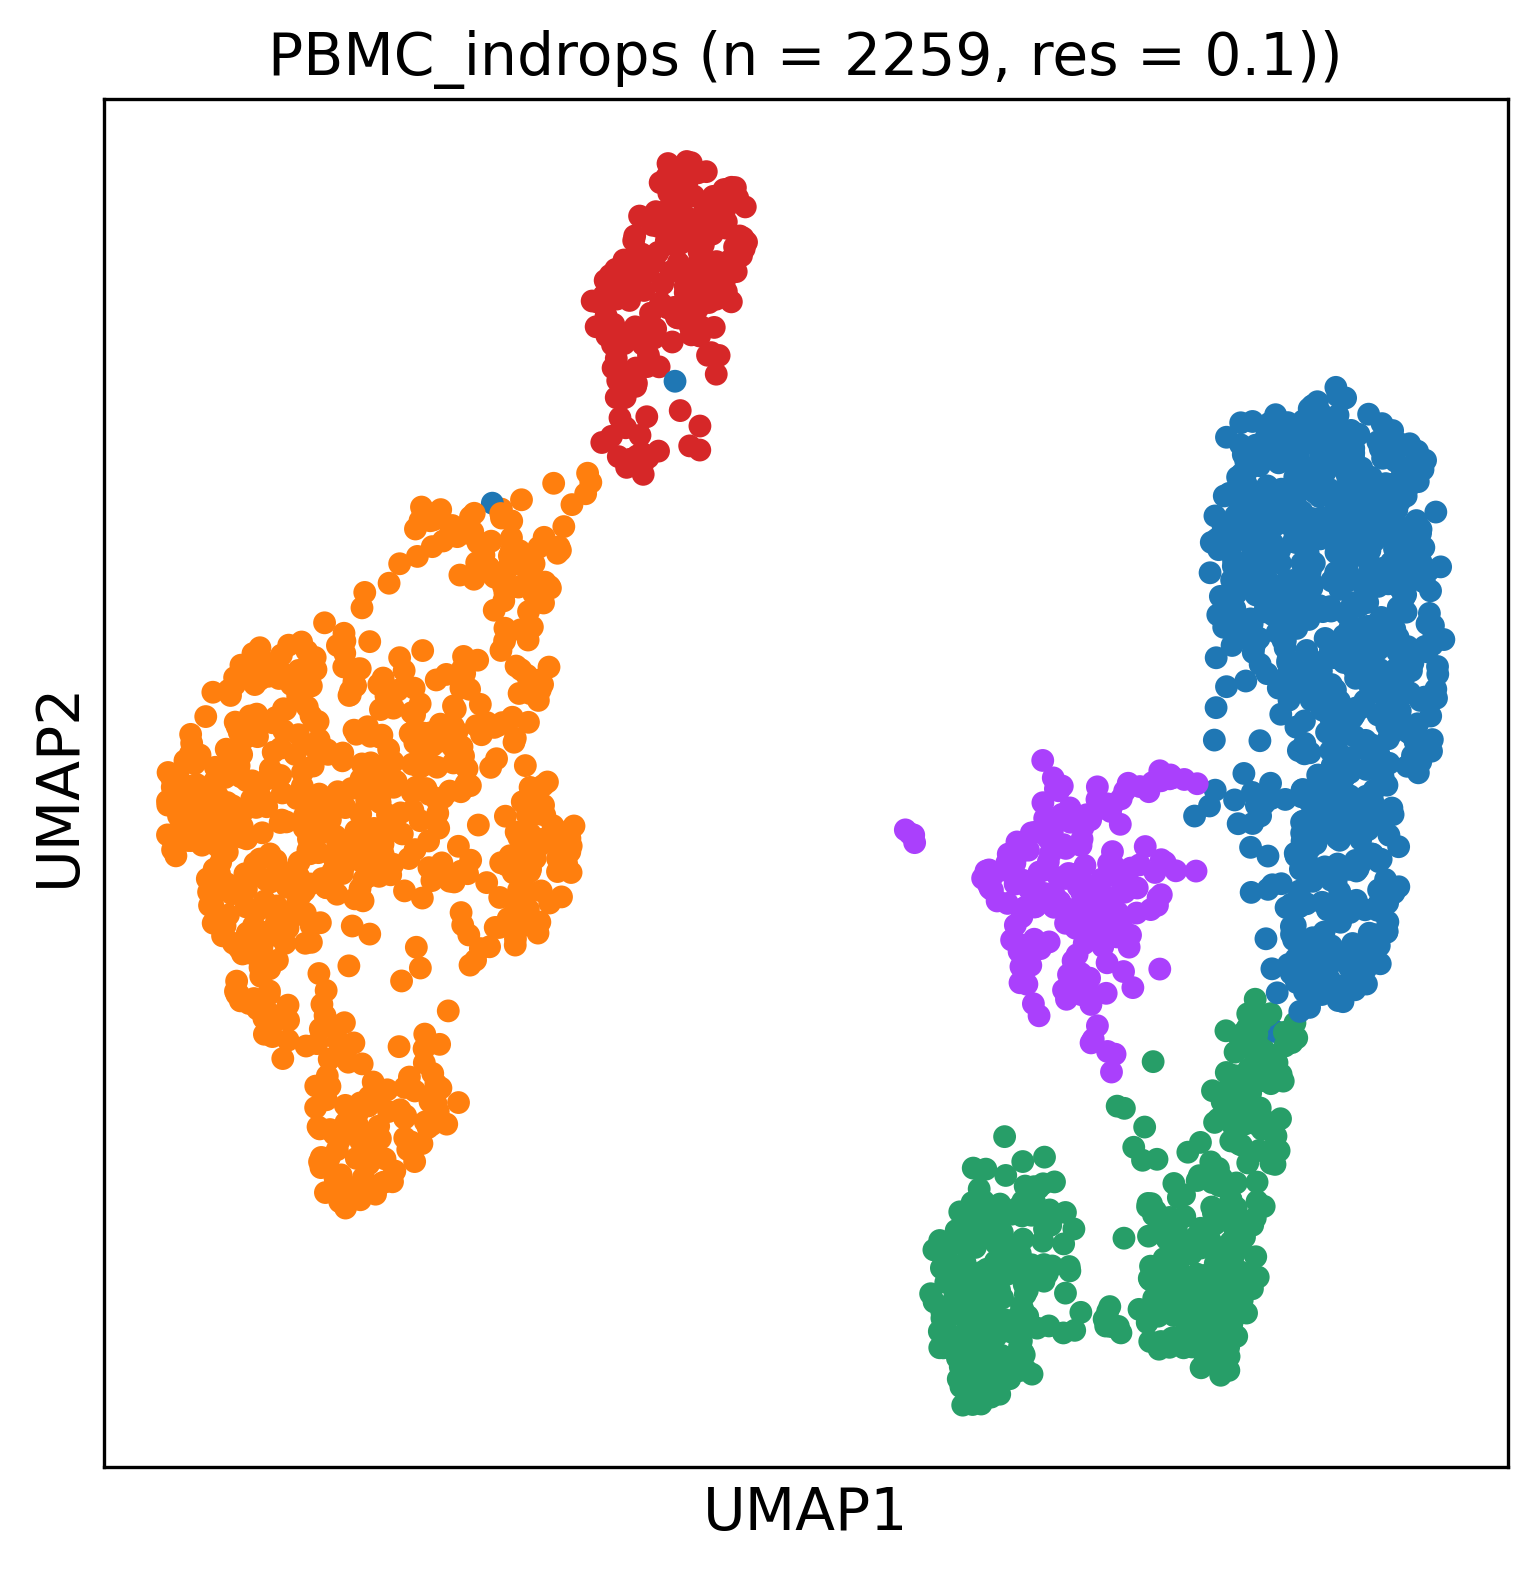
\includegraphics[width=0.25\textwidth]{images/clusterings/PBMC_indrops.png} &
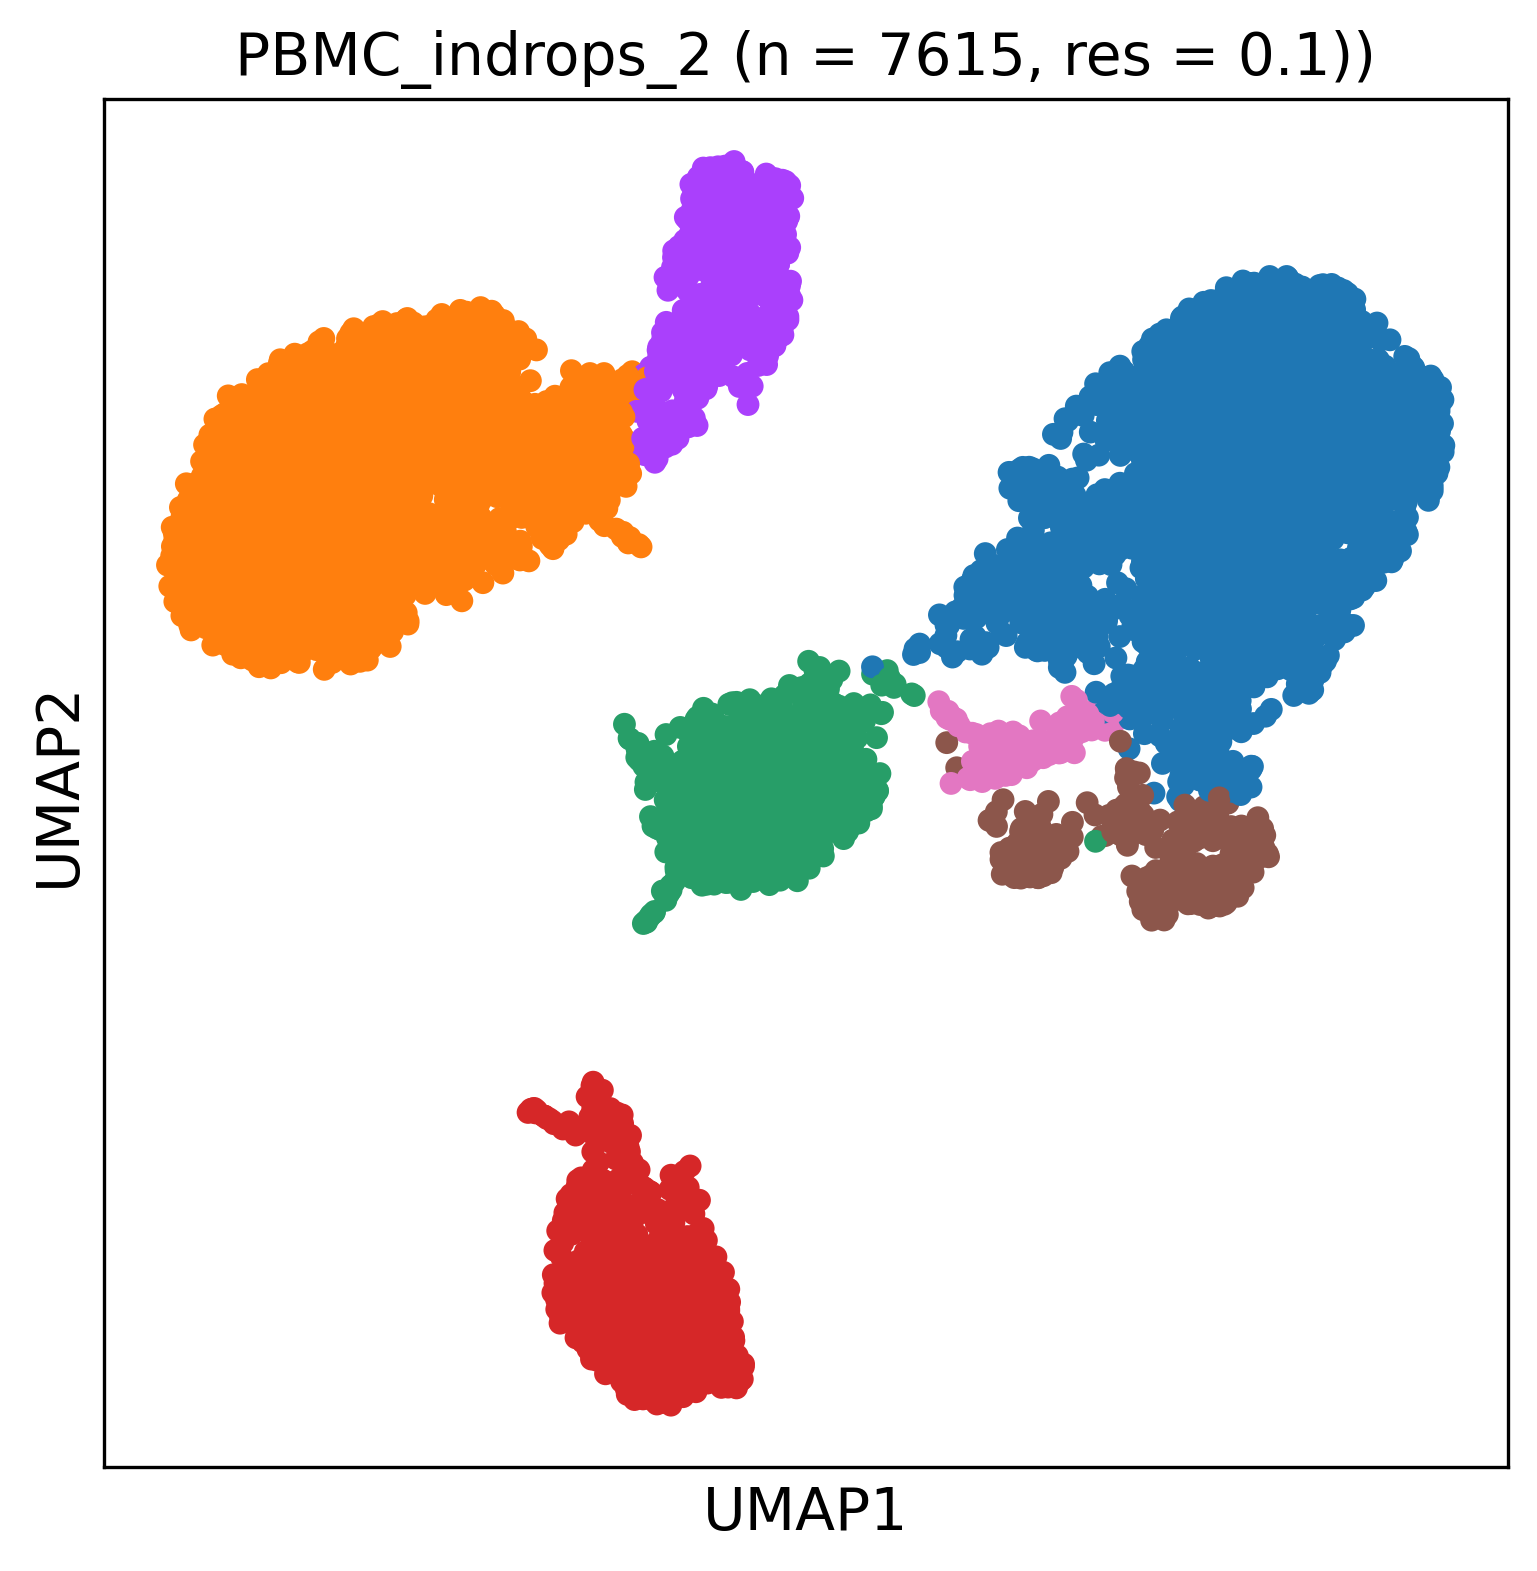
\includegraphics[width=0.25\textwidth]{images/clusterings/PBMC_indrops_2.png} &
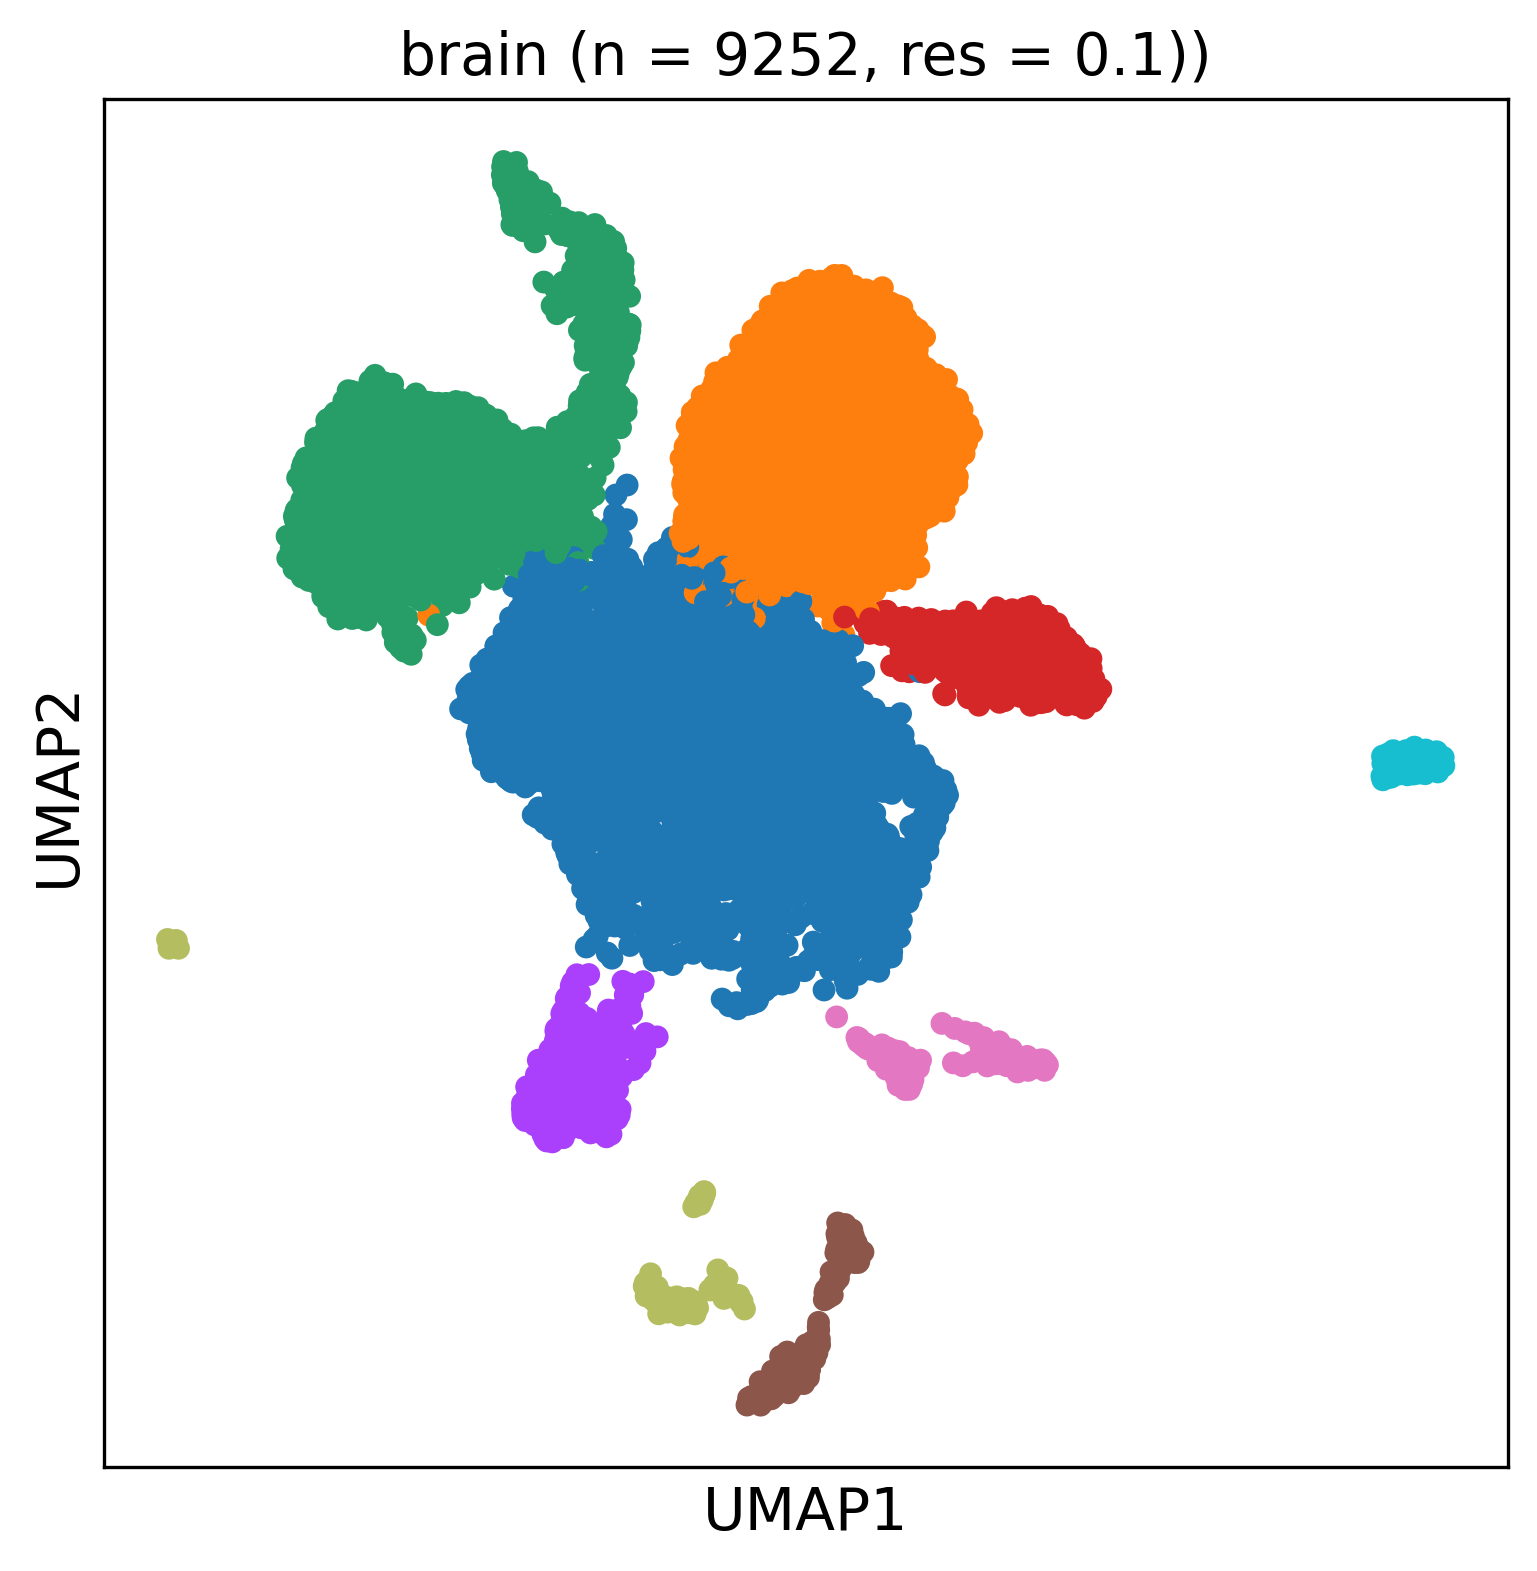
\includegraphics[width=0.25\textwidth]{images/clusterings/brain.png} \\
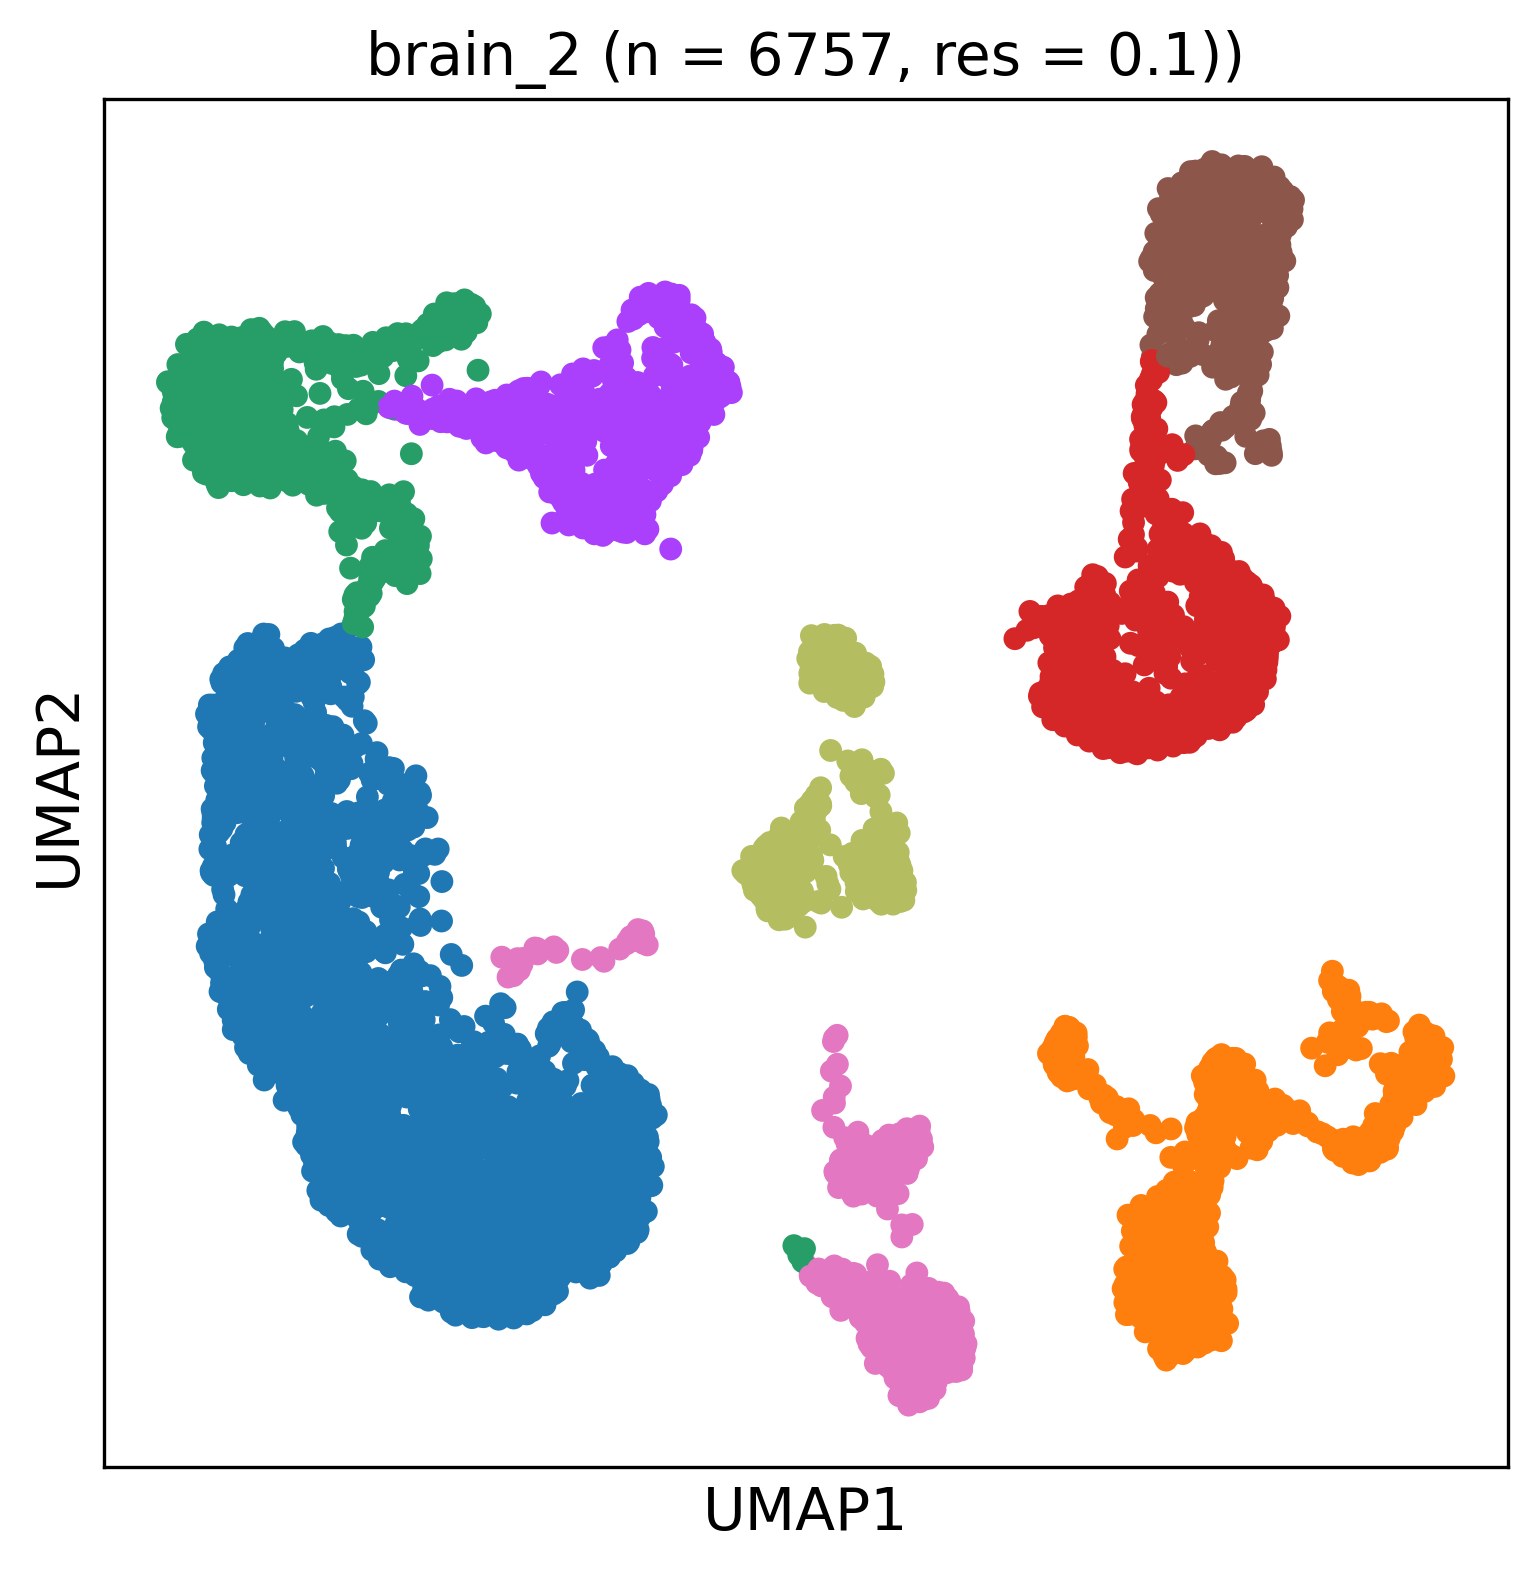
\includegraphics[width=0.25\textwidth]{images/clusterings/brain_2.png} &
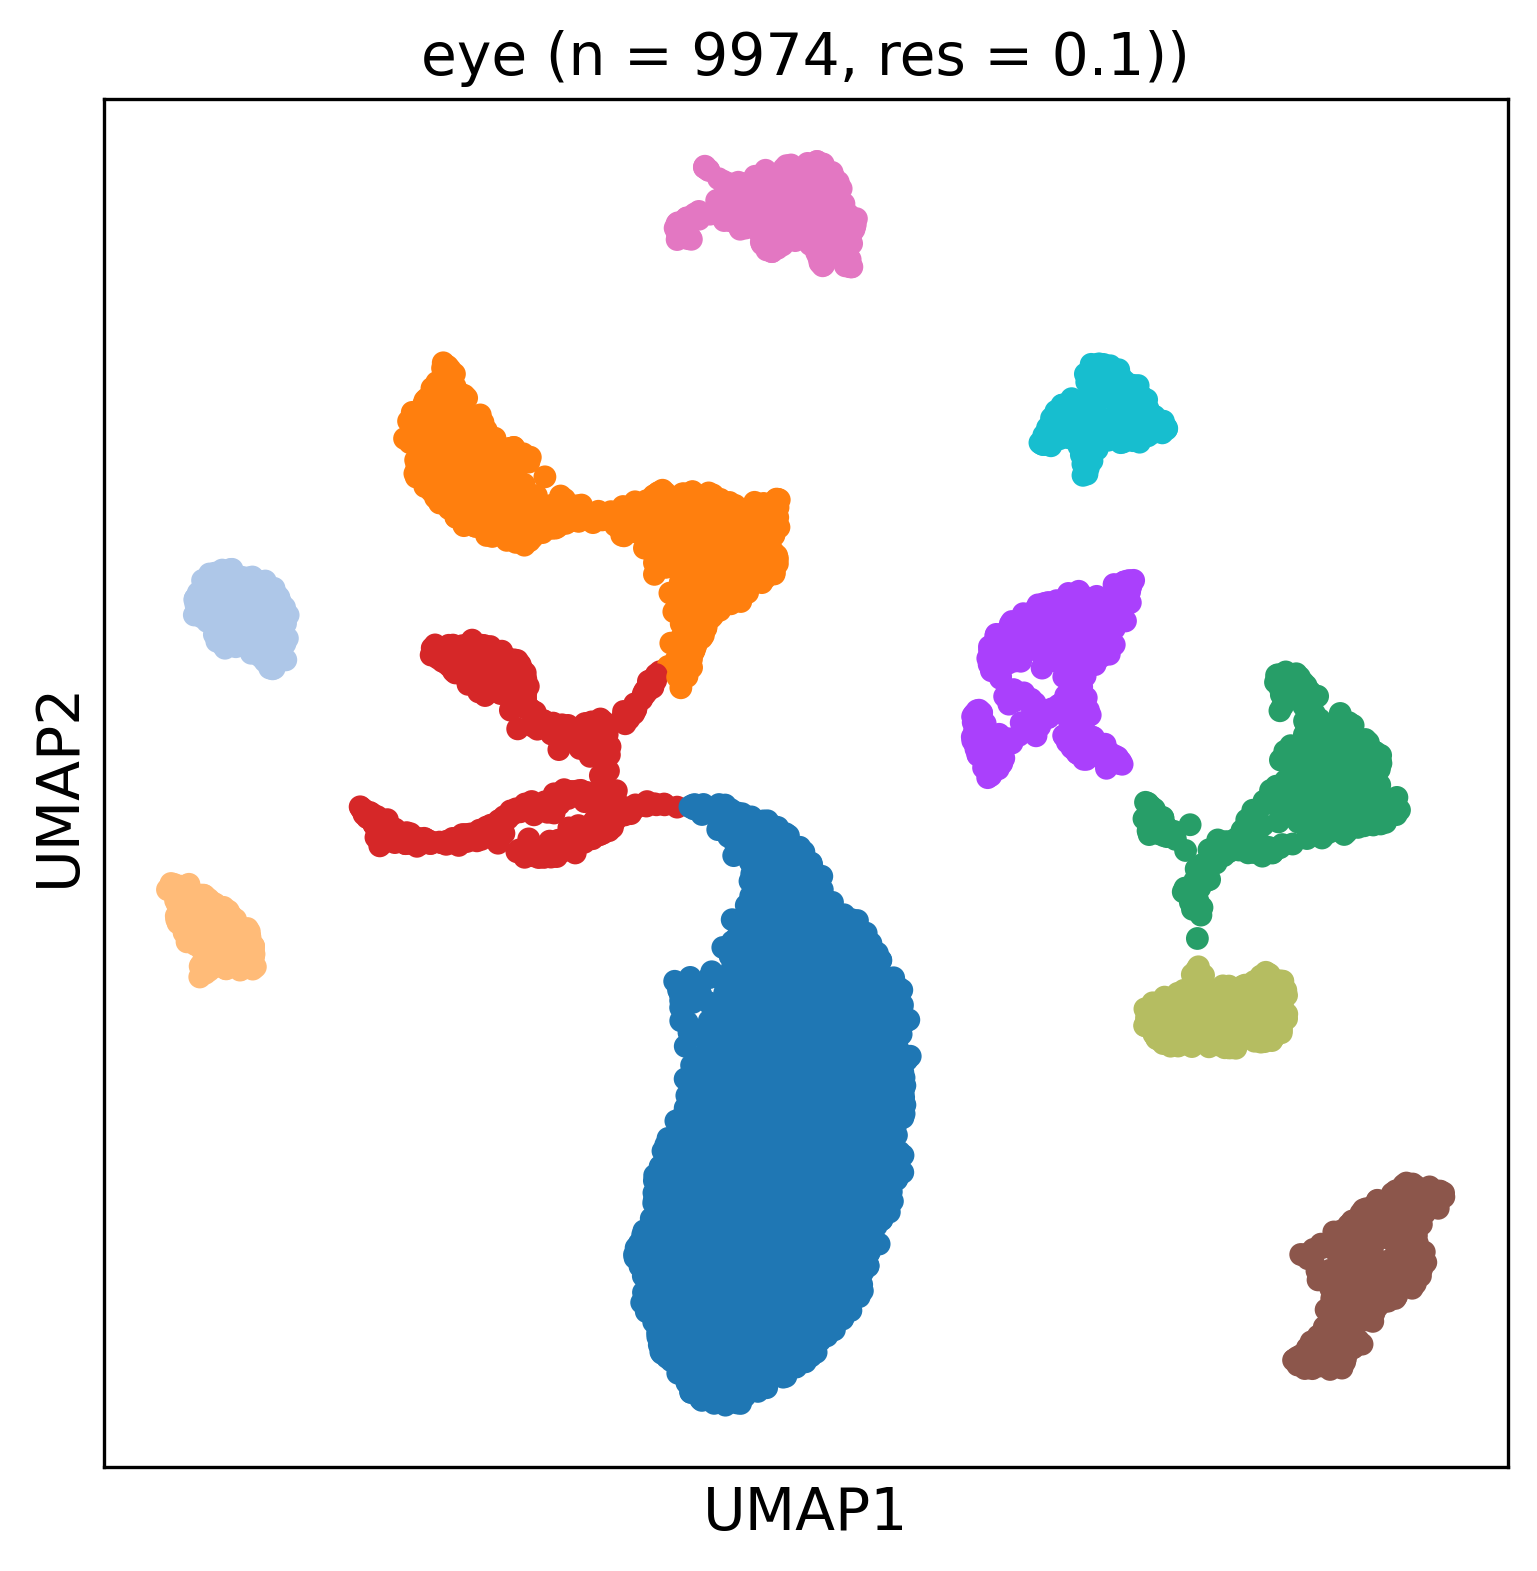
\includegraphics[width=0.25\textwidth]{images/clusterings/eye.png} &
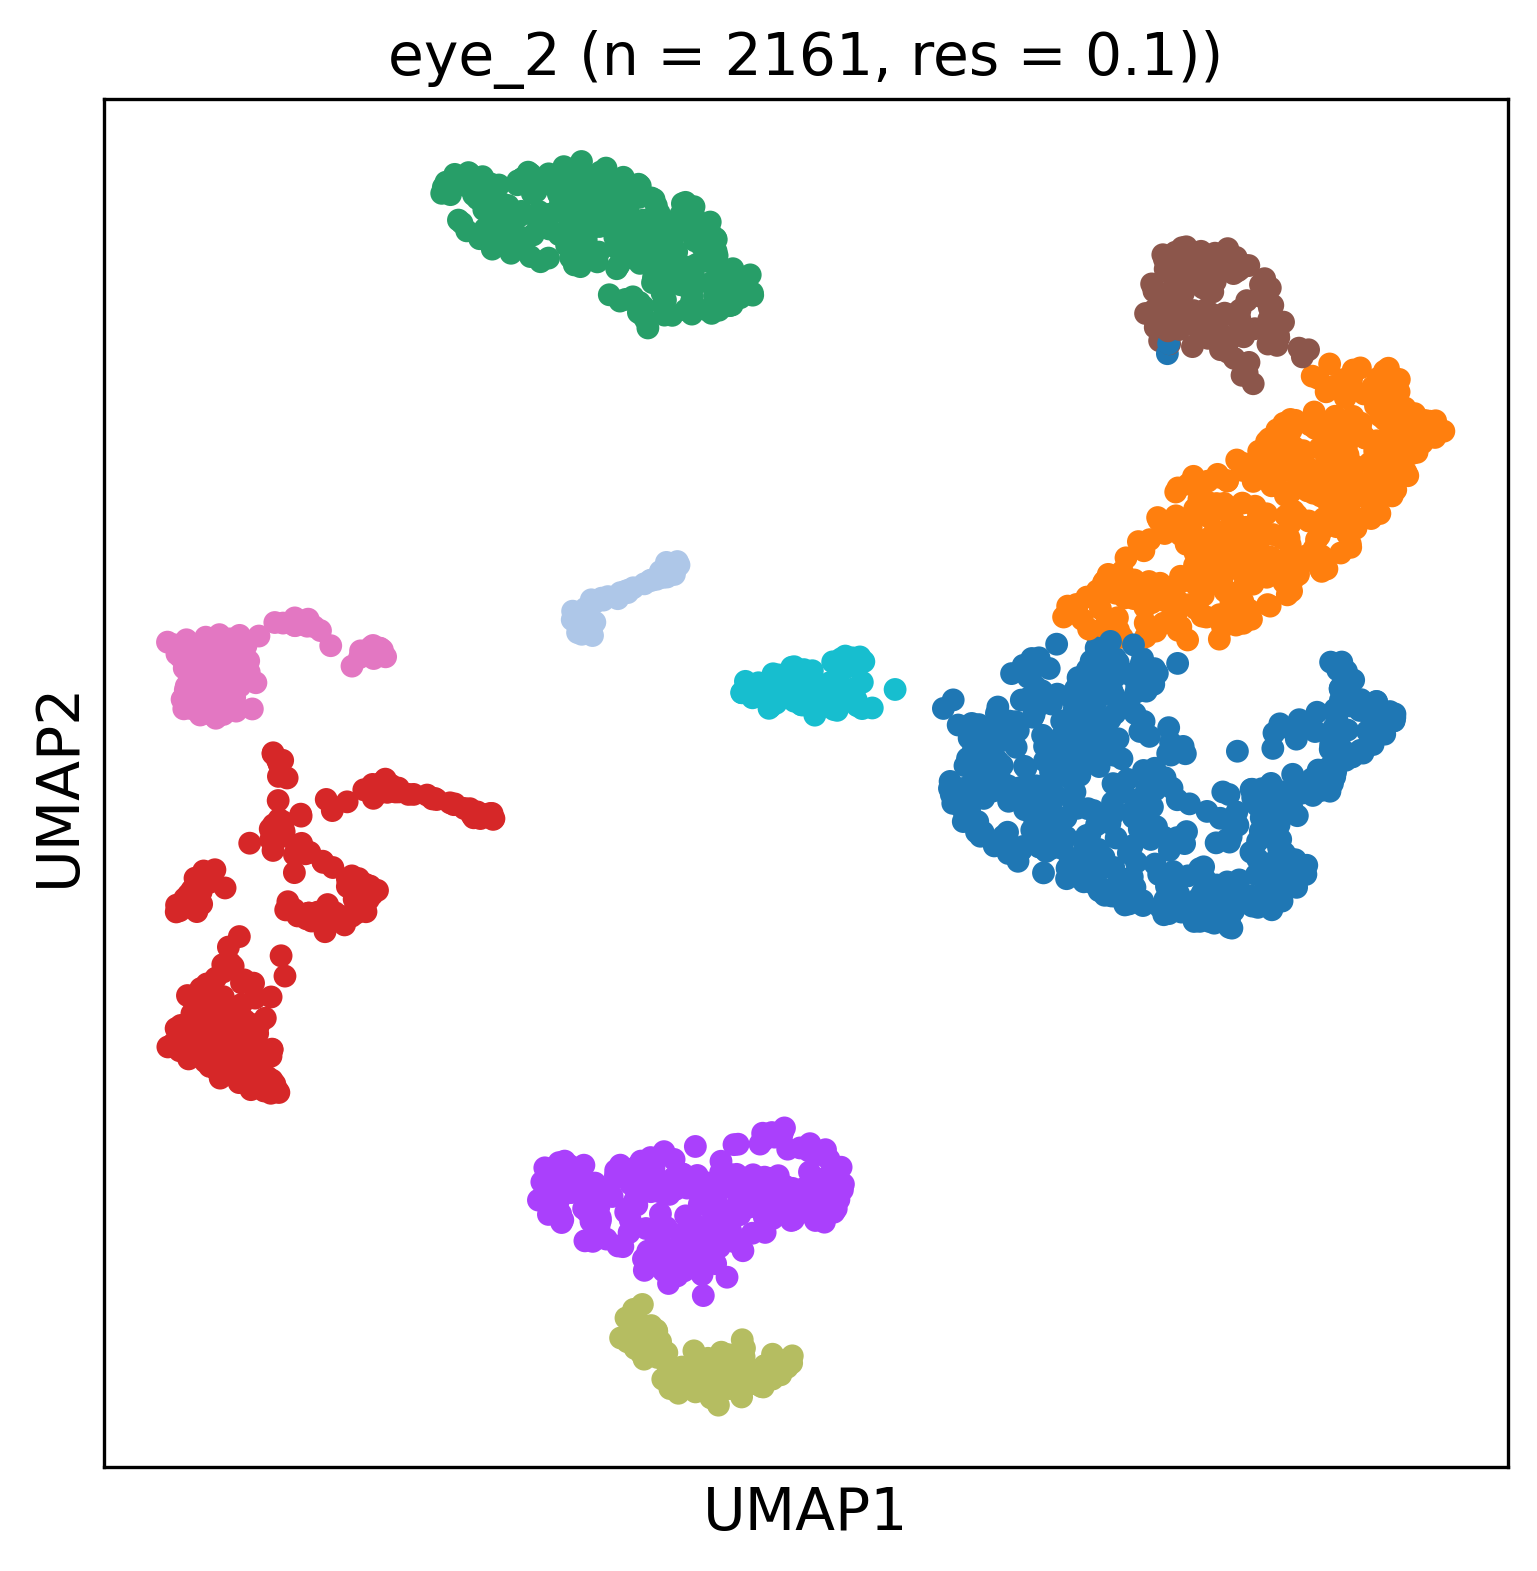
\includegraphics[width=0.25\textwidth]{images/clusterings/eye_2.png} \\
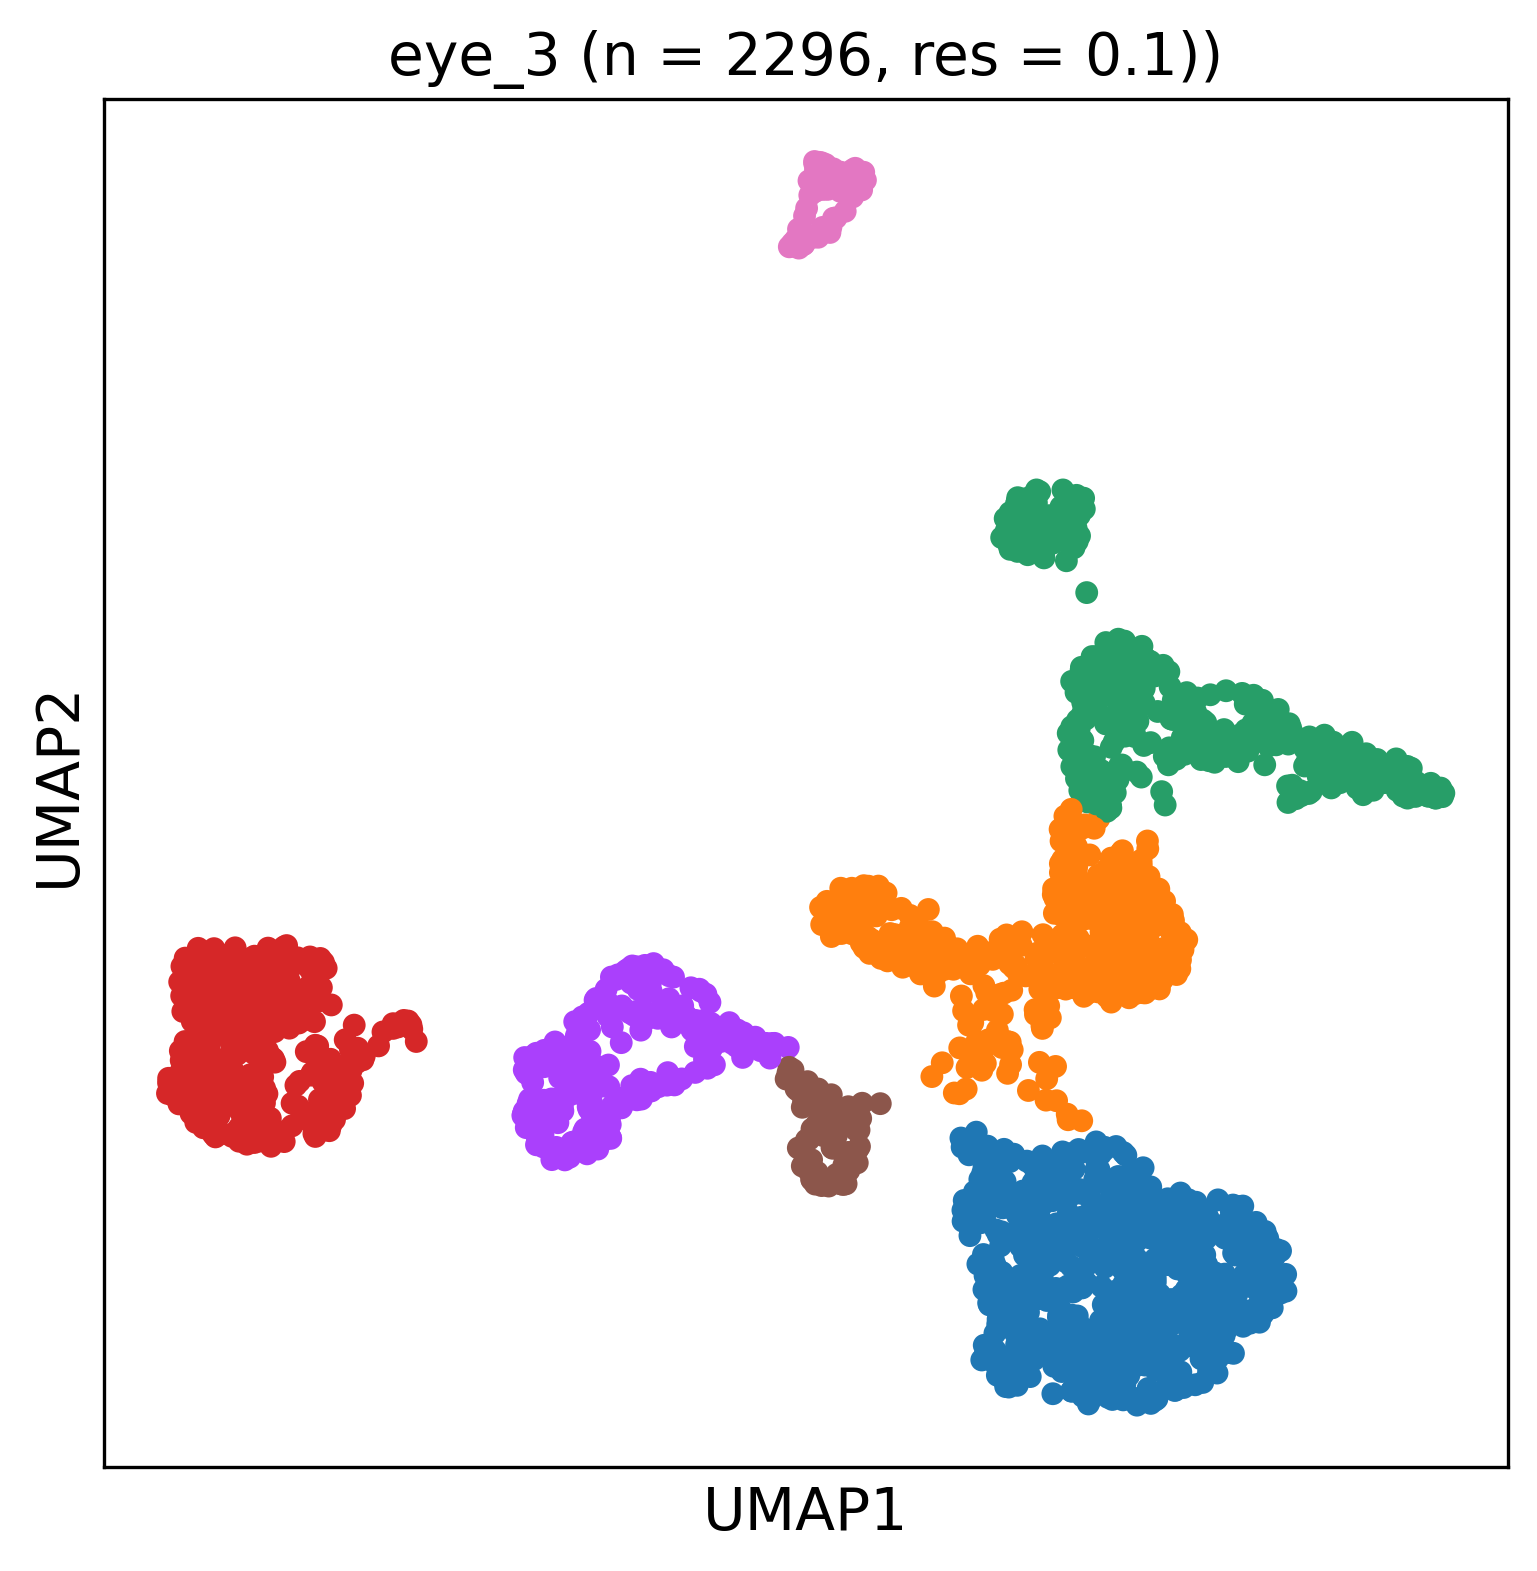
\includegraphics[width=0.25\textwidth]{images/clusterings/eye_3.png} &
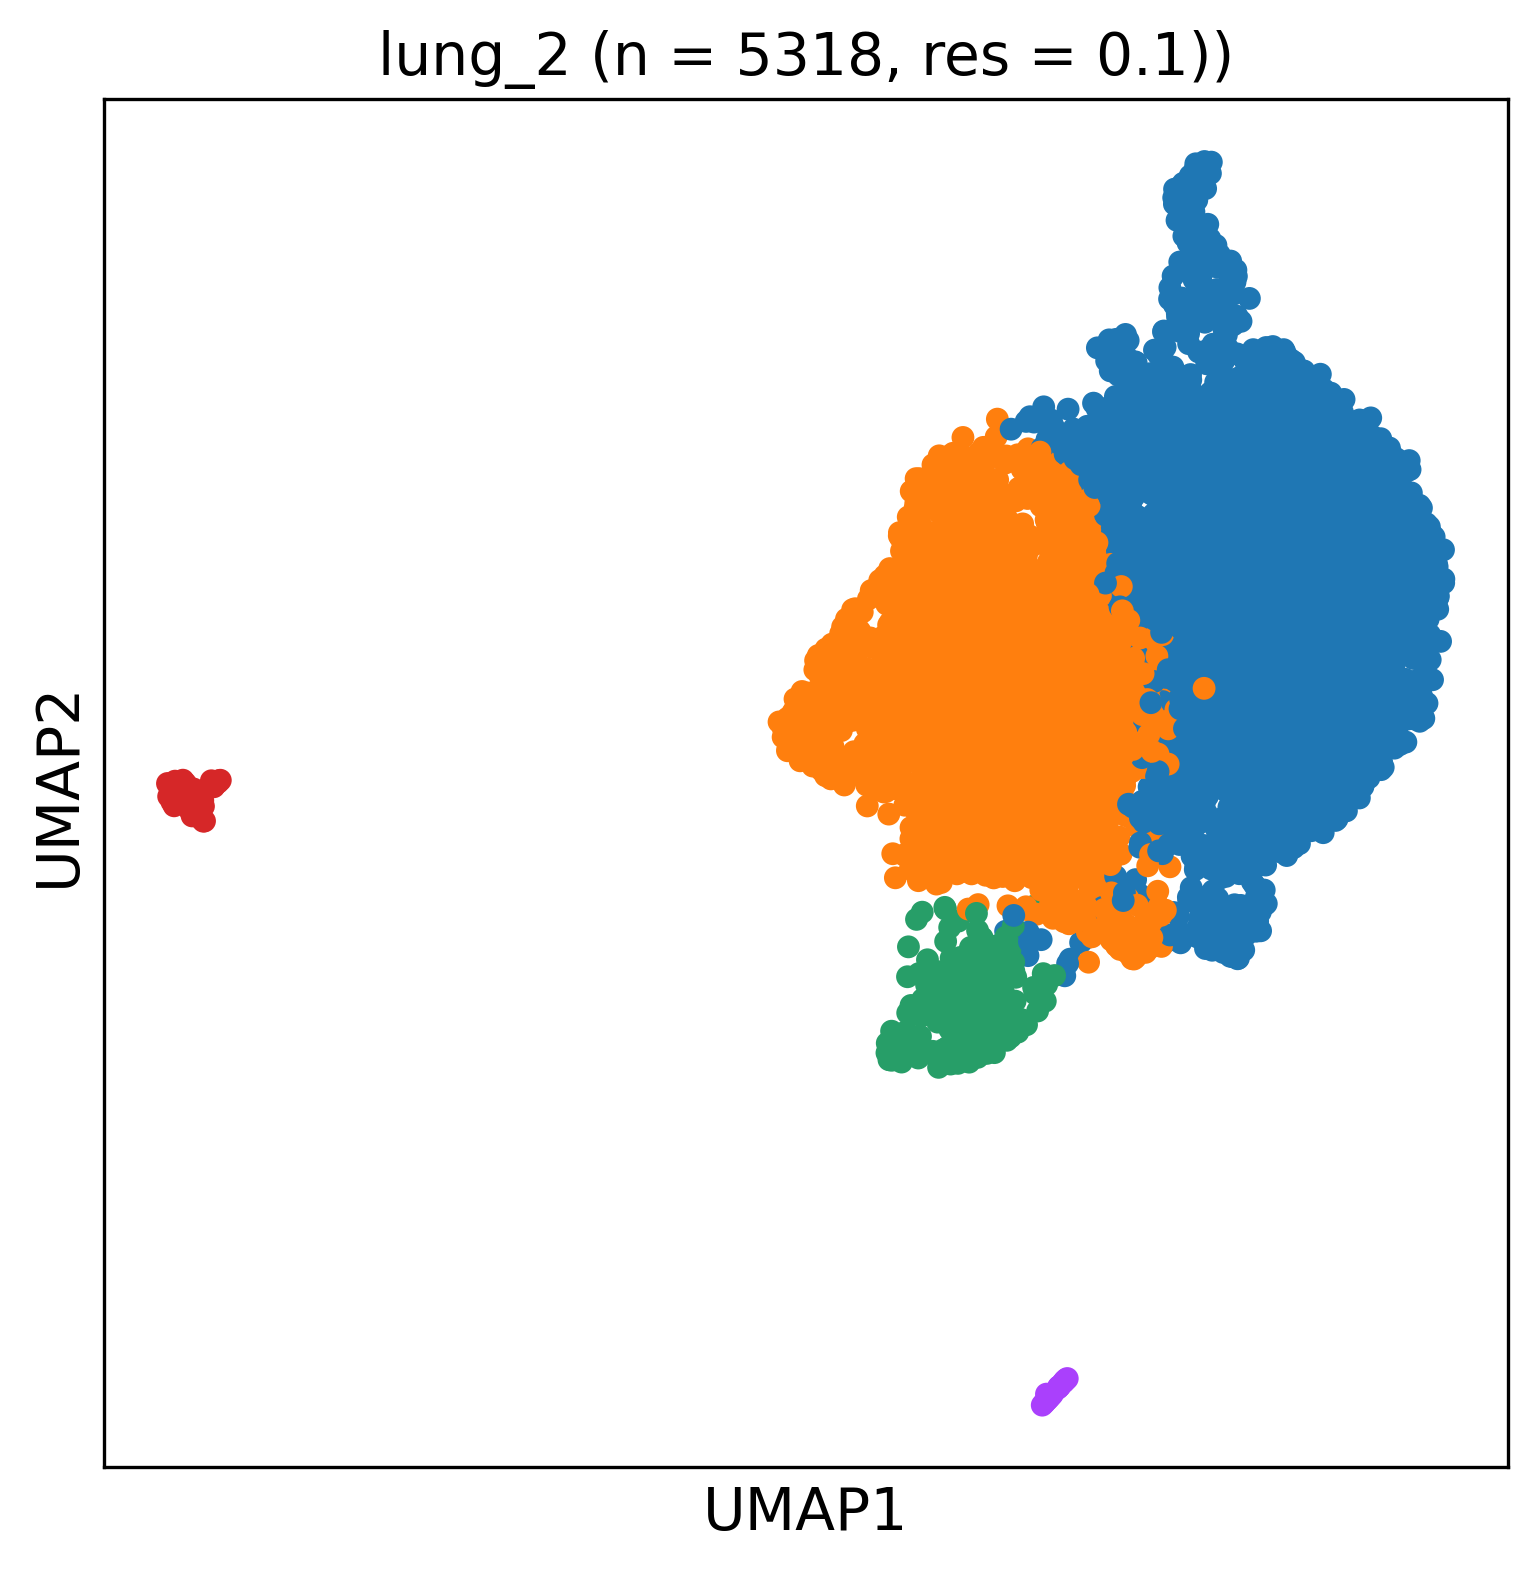
\includegraphics[width=0.25\textwidth]{images/clusterings/lung_2.png} &
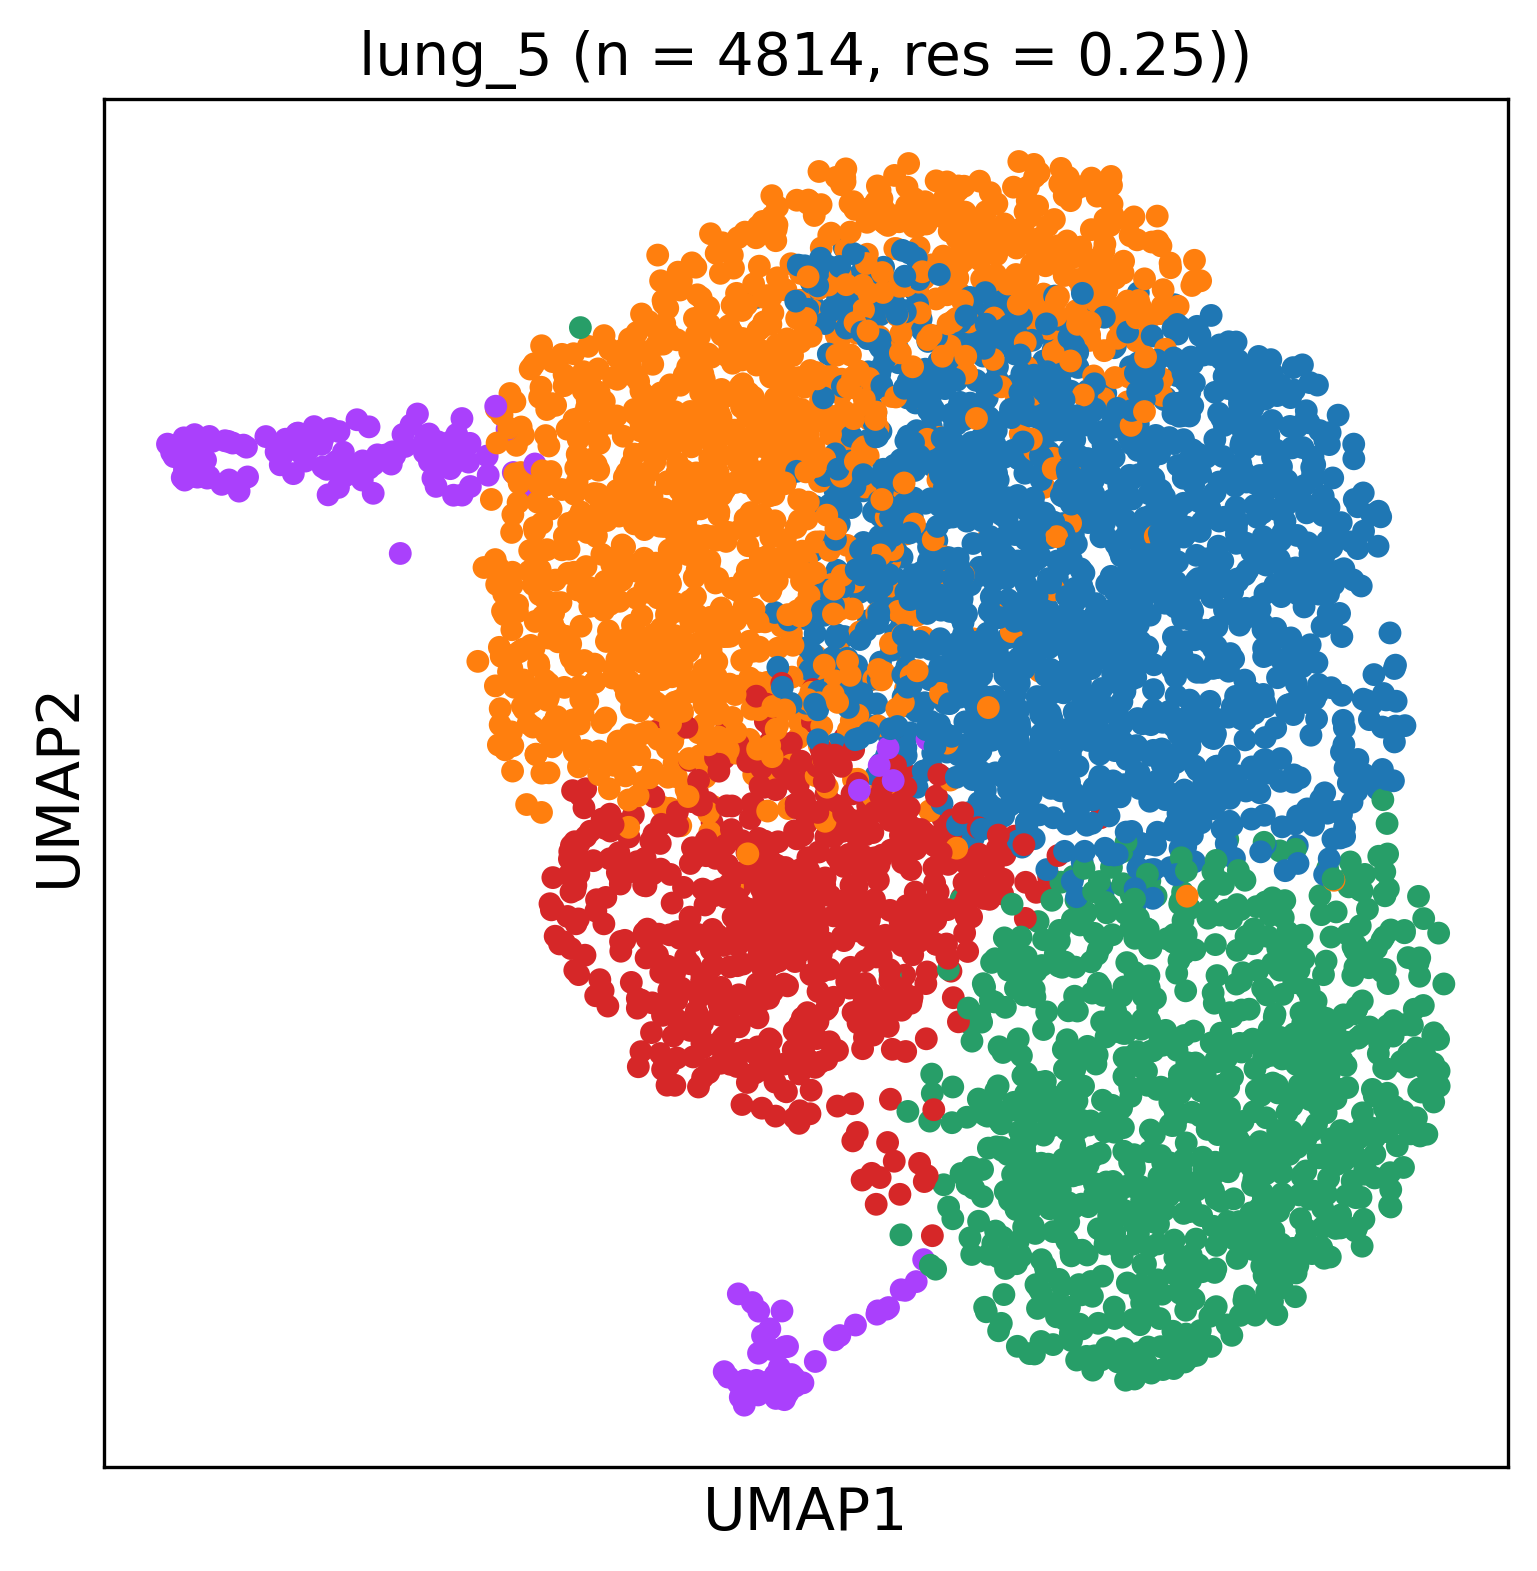
\includegraphics[width=0.25\textwidth]{images/clusterings/lung_5.png} \\
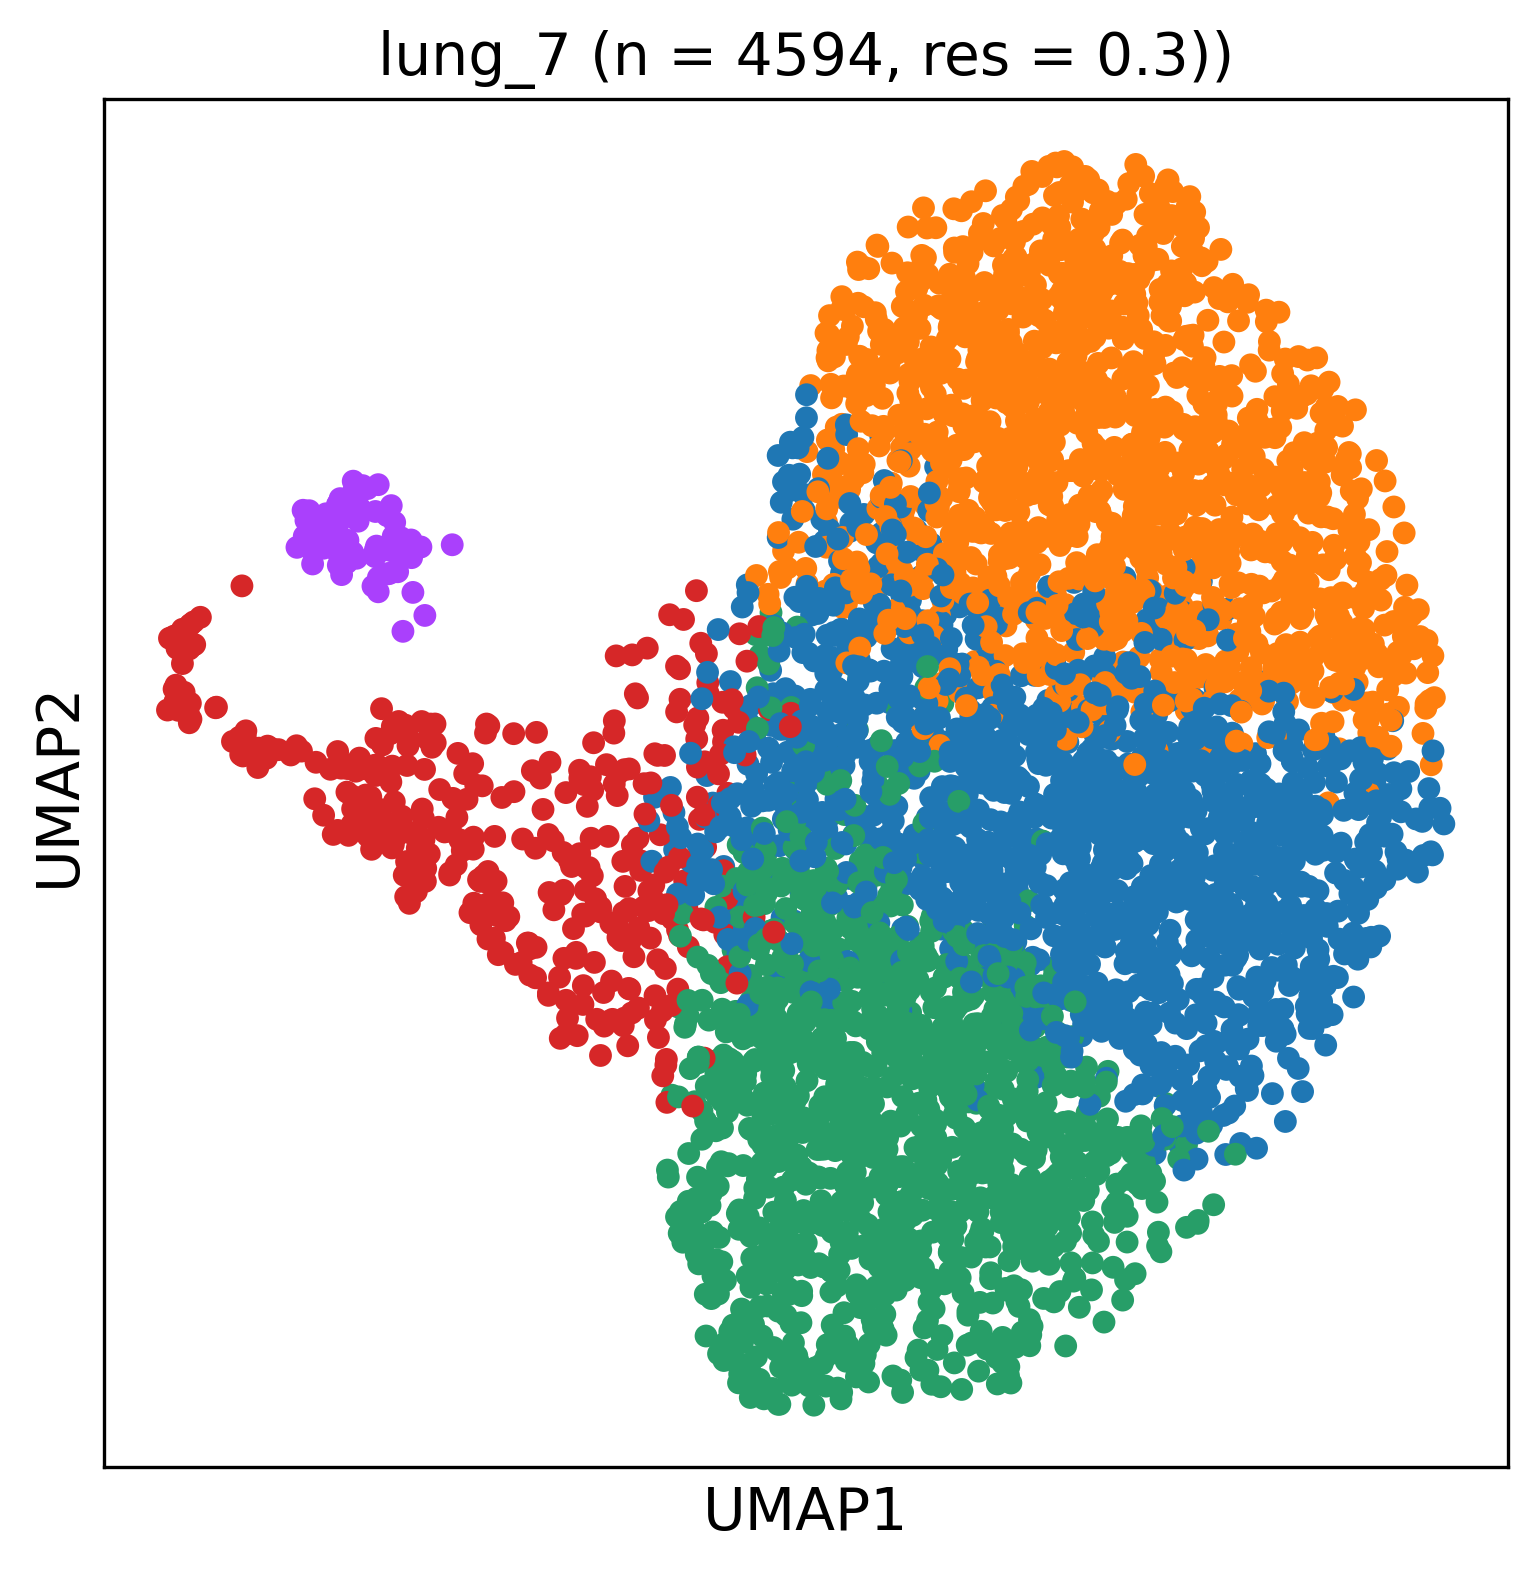
\includegraphics[width=0.25\textwidth]{images/clusterings/lung_7.png} &
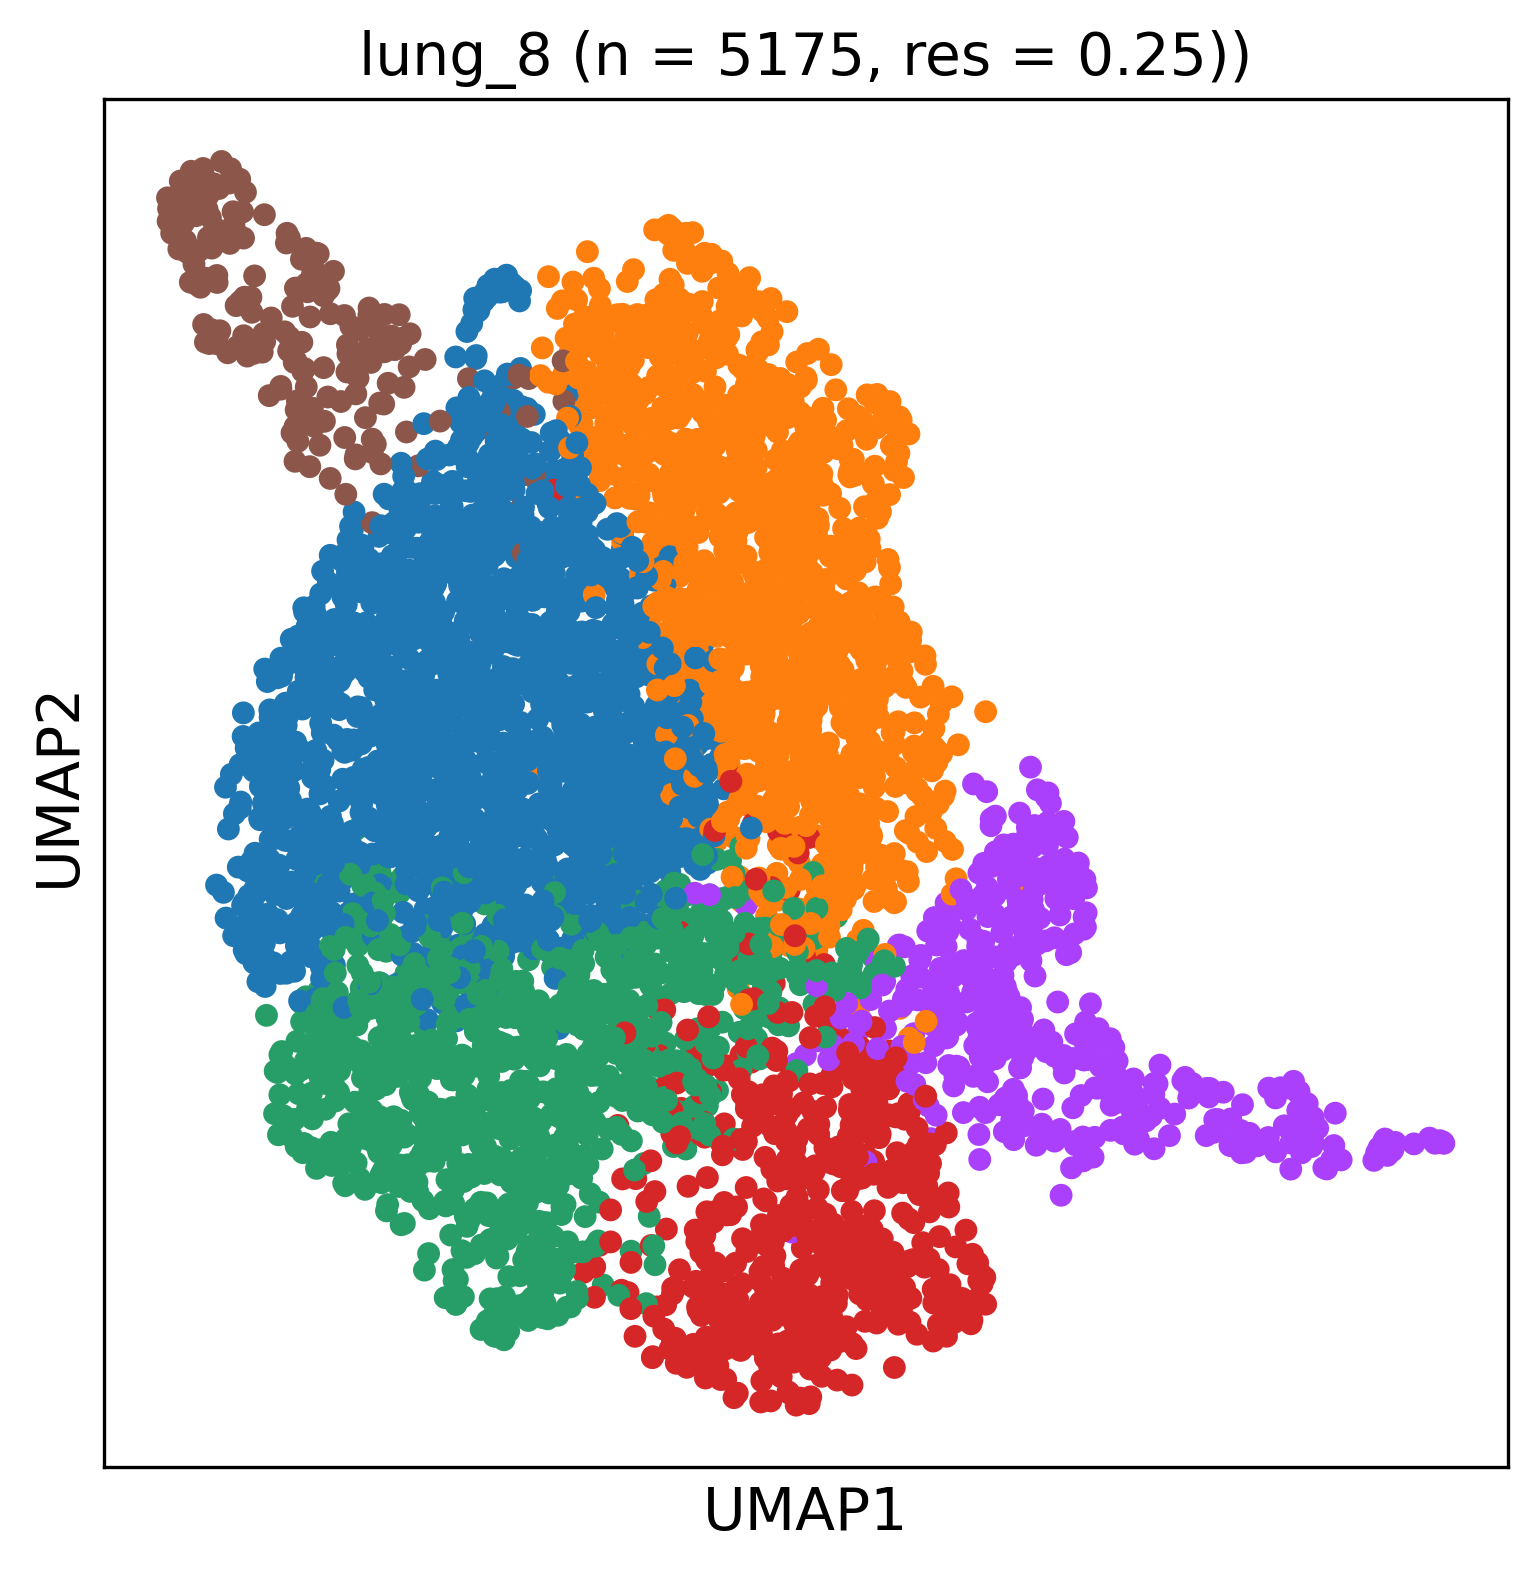
\includegraphics[width=0.25\textwidth]{images/clusterings/lung_8.png} &
\\
\end{tabular}
\end{figure}

\renewcommand{\arraystretch}{1.5}

\begin{longtable}{llccccc}
\caption{Isolated intergenic regions. The DGE column indicates whether the region is differentially expressed. The Predictions column shows whether the region overlaps with a predicted gene. The Conservation column indicates whether the region has a conservation score greater than 0.6. The TATA column shows the distance to the closest TATA box upstream (a dot indicates no TATA box was not found within 10 kb upstream). The Poly-A column shows the distance to the poly-A stretch downstream (negative values indicate cases where the poly-A stretch slightly overlaps with the defined region, dot indicate that such stretch was not found in the 1kb downstream).} 
\label{tab:isolated}\\
\toprule
Name & Coordinates & DGE & Predictions & Conservation & TATA & Poly-A \\
\midrule
\endfirsthead

\toprule
Name & Coordinates & DGE & Predictions & Conservation & TATA & Poly-A \\
\midrule
\endhead

\midrule
\multicolumn{7}{r}{\textit{Continued on next page}} \\
\bottomrule
\endfoot

\bottomrule
\endlastfoot

INT1066 & 16:11540750-11541200 & Yes & No & No & . & -10 \\
INT1312 & 3:141483900-141484100 & Yes & No & No & . & 25 \\
INT1366 & 12:14938950-14939300 & Yes & No & No & . & 33 \\
INT1426 & 12:10148500-10148700 & Yes & No & No & 307 & 21 \\
INT1483 & 16:11541550-11541700 & Yes & No & No & . & 74 \\
INT1492 & X:56386150-56386400 & Yes & No & No & 257 & 42 \\
INT1525 & 8:11842200-11842350 & Yes & Yes & No & . & 67 \\
INT1554 & 14:61119550-61119750 & Yes & No & No & . & 54 \\
INT1609 & 1:149879050-149879250 & Yes & No & No & . & 58 \\
INT1938 & 6:148107250-148107550 & Yes & No & No & . & 17 \\
INT196 & 6:89086200-89086500 & Yes & Yes & No & 713 & -2 \\
INT1993 & 6:43788000-43788200 & Yes & No & No & . & 45 \\
INT2008 & 17:1567900-1568100 & Yes & No & No & . & 22 \\
INT2141 & 6:159668300-159668550 & Yes & No & No & . & 37 \\
INT2209 & 9:93049900-93050150 & Yes & No & No & . & 21 \\
INT2328 & 1:991500-991800 & Yes & No & No & . & -44 \\
INT2456 & 13:113740250-113740500 & Yes & No & No & . & -10 \\
INT3259 & 17:35461800-35462050 & Yes & No & No & 150 & 22 \\
INT349 & 17:43322200-43322700 & Yes & No & No & . & 97 \\
INT368 & 19:14511650-14511900 & Yes & No & No & 231 & 42 \\
INT404 & 2:73747700-73748000 & Yes & No & No & 250 & 13 \\
INT4044 & 1:144412800-144413000 & Yes & No & No & . & . \\
INT4216 & 19:39430250-39430550 & Yes & No & No & . & 17 \\
INT4287 & 17:78646500-78646650 & Yes & No & No & . & 57 \\
INT4872 & 1:12153700-12153900 & Yes & No & No & . & 415 \\
INT5677 & 9:40875600-40875750 & Yes & No & No & . & 185 \\
INT5882 & 7:8754100-8754250 & Yes & No & No & 653 & 124 \\
INT6013 & 2:7102300-7102500 & Yes & No & No & . & 102 \\
INT977 & 1:145987350-145987600 & Yes & No & No & 879 & 37 \\
INT1002 & 5:82392950-82393200 & No & No & No & . & 71 \\
INT1020 & 2:218407950-218408200 & No & No & No & 881 & 59 \\
INT1114 & 21:15897200-15897400 & No & No & No & . & 42 \\
INT1173 & X:81313150-81313400 & No & No & No & 737 & 64 \\
INT1216 & 1:72282700-72282900 & No & Yes & Yes & . & -5 \\
INT127 & 17:32384850-32385100 & No & No & No & 656 & 51 \\
INT1385 & 2:86496700-86496900 & No & No & No & 89 & 12 \\
INT1387 & 11:63570800-63571050 & No & Yes & No & 231 & -26 \\
INT1406 & 14:21194850-21195150 & No & No & No & . & -50 \\
INT1428 & 3:88001700-88001900 & No & No & No & . & 47 \\
INT1467 & 5:112519400-112519600 & No & No & No & 765 & 6 \\
INT1470 & 17:32392900-32393100 & No & No & No & 670 & 118 \\
INT1509 & 2:42067000-42067200 & No & No & No & 95 & 27 \\
INT1527 & 19:7573150-7573300 & No & No & No & . & 38 \\
INT1542 & 18:70815200-70815400 & No & No & No & . & 22 \\
INT1549 & 1:231017800-231018000 & No & No & No & . & 48 \\
INT1569 & 1:157823400-157823600 & No & No & No & . & 11 \\
INT1571 & 10:17913700-17913900 & No & No & No & . & 21 \\
INT1579 & 3:12435200-12435400 & No & No & No & . & 30 \\
INT1618 & 8:16107400-16107550 & No & No & No & 228 & 40 \\
INT1619 & 3:56722050-56722300 & No & No & No & . & 1 \\
INT1637 & 4:81423000-81423200 & No & No & No & 702 & 40 \\
INT1640 & 17:7180650-7180850 & No & No & No & . & 33 \\
INT1675 & 11:65772750-65772950 & No & No & No & . & . \\
INT1716 & 9:27320000-27320200 & No & No & No & . & 49 \\
INT1778 & 2:222711150-222711300 & No & No & No & 96 & 67 \\
INT1779 & 3:189405250-189405400 & No & No & No & 141 & 61 \\
INT1781 & 20:50205450-50205650 & No & No & No & 72 & 36 \\
INT1801 & 5:151272550-151272700 & No & Yes & No & . & 43 \\
INT1817 & 1:42711550-42711800 & No & No & No & . & 29 \\
INT1829 & 1:77772950-77773050 & No & No & Yes & . & -30 \\
INT1869 & 13:30764850-30765000 & No & No & No & . & . \\
INT1970 & 2:55277900-55278150 & No & No & No & 421 & -4 \\
INT2044 & 19:4041150-4041400 & No & Yes & No & . & 22 \\
INT2071 & 15:84812500-84812800 & No & No & No & 773 & 39 \\
INT2080 & 2:218816950-218817250 & No & No & No & . & 111 \\
INT2088 & 8:19876500-19876650 & No & No & No & 699 & . \\
INT212 & X:44794800-44794950 & No & No & No & . & -43 \\
INT2142 & 12:54548650-54548850 & No & No & No & . & 63 \\
INT2162 & 17:16355850-16356050 & No & No & No & . & 46 \\
INT2199 & 6:148122550-148122750 & No & No & Yes & . & 74 \\
INT2208 & 5:18162950-18163100 & No & No & Yes & . & 93 \\
INT225 & 9:131570800-131571100 & No & No & No & 400 & -23 \\
INT2389 & 22:17731150-17731400 & No & No & No & 818 & 26 \\
INT2420 & 1:52681350-52681600 & No & No & No & 980 & 52 \\
INT2448 & 15:77040800-77041050 & No & No & No & . & 47 \\
INT2585 & 17:75300550-75300800 & No & No & No & 473 & 12 \\
INT2716 & 7:39812450-39812600 & No & No & No & . & 108 \\
INT2777 & 12:106347650-106347900 & No & No & No & . & 50 \\
INT2826 & 3:156825050-156825300 & No & No & No & 254 & 47 \\
INT2970 & 1:30727150-30727450 & No & No & No & . & 3 \\
INT312 & 9:127792200-127792400 & No & No & No & . & 57 \\
INT313 & 20:5540550-5540800 & No & No & No & . & 20 \\
INT316 & 2:157407250-157407500 & No & No & No & 237 & 42 \\
INT3329 & 12:124911350-124911600 & No & No & No & . & 19 \\
INT3330 & 10:26574800-26575050 & No & No & No & 107 & 39 \\
INT3432 & 11:2318900-2319500 & No & No & No & . & 32 \\
INT3472 & 1:234336450-234336650 & No & No & No & 516 & 80 \\
INT3506 & 2:94568900-94569100 & No & No & No & 601 & . \\
INT3519 & 5:166646400-166646600 & No & No & No & 273 & 121 \\
INT3521 & 1:234330500-234330750 & No & No & No & 767 & 97 \\
INT3543 & 13:83860250-83860700 & No & No & No & 836 & -25 \\
INT3636 & X:129412750-129413050 & No & No & Yes & . & 107 \\
INT3657 & 10:95078350-95078550 & No & No & No & 255 & 110 \\
INT3658 & 11:29999550-29999750 & No & No & No & 760 & 98 \\
INT3668 & 5:120107300-120107650 & No & No & No & . & -21 \\
INT3671 & 16:56859450-56859650 & No & No & No & . & 116 \\
INT3704 & 18:43159050-43159250 & No & No & No & 70 & 104 \\
INT3759 & X:129426200-129426450 & No & No & No & . & 108 \\
INT3940 & 4:157391550-157391750 & No & No & No & . & 96 \\
INT4032 & 3:15548800-15549000 & No & No & No & 843 & 121 \\
INT4047 & 21:33361700-33361900 & No & No & No & 143 & 39 \\
INT4070 & 4:47430500-47430700 & No & Yes & No & 934 & 90 \\
INT4147 & 1:34861500-34861700 & No & Yes & No & . & 609 \\
INT4174 & 7:128664300-128664550 & No & No & No & 439 & 39 \\
INT4224 & 8:43139250-43139600 & No & No & No & . & . \\
INT4225 & 6:110097900-110098100 & No & No & No & 115 & 95 \\
INT4236 & X:121756550-121756750 & No & No & No & . & 83 \\
INT426 & 14:24169950-24170200 & No & No & No & . & 29 \\
INT4328 & 17:45610750-45610900 & No & No & No & 835 & 80 \\
INT4364 & Y:20418250-20418500 & No & No & No & 241 & 49 \\
INT4394 & 19:40026900-40027100 & No & No & No & . & 89 \\
INT4401 & 9:101413900-101414100 & No & No & No & . & 47 \\
INT4454 & X:57773350-57773500 & No & No & No & 191 & 136 \\
INT4488 & 9:41567350-41567550 & No & No & No & 304 & -23 \\
INT4525 & 12:11599200-11599400 & No & No & No & 776 & 19 \\
INT4577 & 5:702050-702300 & No & Yes & No & 893 & 86 \\
INT4610 & 2:7218550-7218750 & No & No & No & 90 & 53 \\
INT4697 & 5:166509150-166509400 & No & No & No & 14 & 55 \\
INT4706 & 13:19811450-19811650 & No & No & No & 22 & 108 \\
INT480 & 17:32396150-32396400 & No & No & No & 137 & 26 \\
INT4851 & X:129410350-129410550 & No & No & No & . & 94 \\
INT4924 & 20:33358150-33358400 & No & No & No & . & 46 \\
INT4948 & 5:703250-703450 & No & Yes & No & . & . \\
INT4955 & 8:40521250-40521500 & No & No & No & 5 & 76 \\
INT4975 & 12:47660700-47660950 & No & No & No & 71 & . \\
INT5017 & 18:5389700-5389900 & No & No & No & . & 94 \\
INT5128 & 16:67010550-67010750 & No & No & No & . & 81 \\
INT5190 & 18:5386900-5387050 & No & No & No & . & 125 \\
INT5456 & 11:1269150-1269350 & No & No & No & . & 115 \\
INT5524 & 19:46024000-46024250 & No & No & No & 287 & 73 \\
INT560 & 6:32862450-32862700 & No & No & No & 102 & 34 \\
INT5710 & 4:47428500-47428700 & No & Yes & No & 594 & 91 \\
INT575 & 11:85955150-85955450 & No & No & No & . & -6 \\
INT5801 & 16:67010700-67010900 & No & No & No & 949 & . \\
INT5808 & 5:26875600-26875800 & No & No & No & 926 & 109 \\
INT584 & 2:171768300-171768600 & No & No & No & 768 & 13 \\
INT5848 & 16:3239750-3239950 & No & No & No & 488 & 35 \\
INT593 & 2:32331000-32331250 & No & No & No & 814 & 36 \\
INT600 & 22:47183900-47184150 & No & No & No & 22 & 59 \\
INT6019 & 3:49344550-49344850 & No & No & No & . & 57 \\
INT620 & 21:15883150-15883400 & No & No & No & . & 20 \\
INT801 & 15:44718950-44719200 & No & No & No & 386 & 10 \\
INT827 & 9:94111950-94112200 & No & Yes & No & 336 & 55 \\
INT896 & 2:98598550-98598850 & No & No & No & . & 11 \\
INT904 & 2:26138650-26138950 & No & No & No & . & 41 \\
INT906 & 14:92696800-92697050 & No & No & No & . & 18 \\
INT925 & 18:51087400-51087650 & No & No & No & 855 & 17 \\





\end{longtable}



\end{document}
